\documentclass[
    iai, % Saisir le nom de l'institut rattaché
    il, % Saisir le nom de l'orientation
    %confidential, % Décommentez si le travail est confidentiel
]{heig-tb}

\usepackage[nooldvoltagedirection,european,americaninductors]{circuitikz}
\usepackage{tabularx}
\usepackage{graphicx}
\usepackage{comment}
\usepackage{pdfpages}
\usepackage{lscape}

\signature{signature_alec_berney.svg}

\makenomenclature
\makenoidxglossaries
\makeindex

\addbibresource{bibliography.bib}

\input{nomenclature}
\input{acronyms}
\newglossaryentry{heig-vd}{
    name=HEIG-VD,
    description={Haute École d'Ingénierie et de Gestion du canton de Vaud}
}
\newglossaryentry{hes-so}{
    name=HES-SO,
    description={Haute École Supérieure de Suisse Occidentale}
}
\newglossaryentry{latex}{
    name=latex,
    description={Un langage et un système de composition de documents}
}
\newglossaryentry{maths}{
    name=mathematics,
    description={Les mathematiques sont ce que les mathématiciens fonts}
}
\newglossaryentry{docker}{
    name=Docker,
    description={Docker est un outil permettant de gérer des containers, une sorte de machine virtuelle plus légère ayant pour but d'encapsuler une ou plusieurs applications / outils technologiques ainsi que toutes les dépendances que ces dernières exigent pour leur bon fonctionnement}
}
\newglossaryentry{kubernetes}{
    name=Kubernetes,
    description={Kubernetes est un système open-source permettant d'automatiser le déploiement, la mise à l'échelle et la gestion des applications conteneurisées}
}
\newglossaryentry{devops}{
    name=DevOps,
    description={Défini tout le processus conteant l'intégration continue, le déploiement continu et la livraison continue}
}
\newglossaryentry{ci}{
    name=CI,
    description={Continuous Integration / Intégration continue}
}
\newglossaryentry{cd}{
    name=CD,
    description={Continuous Deployement / Déploiement continu}
}
\newglossaryentry{github}{
    name=Github,
    description={GitHub is a website and cloud-based service that helps developers store and manage their code, as well as track and control changes to their code}
}
\newglossaryentry{gitlab}{
    name=Gitlab,
    description={GitLab is The DevOps Platform, delivered as a single application. This makes GitLab unique and creates a streamlined software workflow, unlocking your organization from the constraints of a pieced together toolchain}
}
\newglossaryentry{sgbd}{
    name=SGBD,
    description={Système de Gestion de Base de Données (DBMS), logiciel système servant à stocker, à manipuler ou gérer, et à partager des données dans une base de données}
}
\newglossaryentry{mysql}{
    name=MySQL,
    description={Système de gestion de bases de données relationnelles (SGBDR)}
}
\newglossaryentry{fablab}{
    name=Fablab,
    description={Laboratoire permettant tout type de travaux situé à la HEIG-VD }
}
\newglossaryentry{teams}{
    name=Microsoft Teams,
    description={Plateforme collaborative de visioconférence appartenant à Microsoft}
}
\newglossaryentry{backend}{
    name=Backend,
    description={Terme désignant un étage de sortie d'un logiciel devant produire un résultat. On l'oppose au front-end (aussi appelé un frontal) qui lui est la partie visible de l'iceberg}
}
\newglossaryentry{frontend}{
    name=Frontend,
    description={Partie frontale du projet affichant l'interface utilisateur permettant d'utiliser la logique du backen}
}
\newglossaryentry{bd}{
    name=BD,
    description={Une base de données permet de stocker et de retrouver des données structurées, semi-structurées ou des données brutes ou de l'information, souvent en rapport avec un thème ou une activité. Celles-ci peuvent être de natures différentes et plus ou moins reliées entre elles}
}
\newglossaryentry{rest}{
    name=REST,
    description={REST (representational state transfer) est un style d'architecture logicielle définissant un ensemble de contraintes à utiliser pour créer des services web}
}
\newglossaryentry{api}{
    name=API,
    description={Une interface de programmation d’applications ou interface de programmation applicative (souvent désignée par le terme API pour Application Programming Interface) est un ensemble normalisé de classes, de méthodes, de fonctions et de constantes qui sert de façade par laquelle un logiciel offre des services à d'autres logiciels}
}
\newglossaryentry{framework}{
    name=Framework,
    description={En programmation informatique, un framework est un ensemble cohérent de composants logiciels structurels qui sert à créer les fondations ainsi que les grandes lignes de tout ou partie d'un logiciel, c'est-à-dire une architecture}
}
\newglossaryentry{php}{
    name=PHP,
    description={Language de programmation web}
}
\newglossaryentry{laravel}{
    name=Laravel,
    description={Framework web utilisant le language de programmation php}
}
\newglossaryentry{template}{
    name=Template,
    description={Modèle de projet web frontend définissant déjà toute l'interface graphique et étant adaptable au besoin}
}
\newglossaryentry{javascript}{
    name=JavaScript,
    description={Language de programmation web}
}
\newglossaryentry{vuejs}{
    name=Vue.js,
    description={Framework web frontend utilisant le language de programmation Javascript}
}
\newglossaryentry{nodejs}{
    name=Node.js,
    description={Environnement d’exécution JavaScript construit sur le moteur JavaScript V8}
}
\newglossaryentry{ide}{
    name=IDE,
    description={Un environnement de développement est un ensemble d'outils qui permet d'augmenter la productivité des programmeurs qui développent des logiciels}
}
\newglossaryentry{os}{
    name=OS,
    description={En informatique, un système d'exploitation (souvent appelé OS — de l'anglais Operating System) est un ensemble de programmes qui dirige l'utilisation des ressources d'un ordinateur par des logiciels applicatifs}
}
\newglossaryentry{conteneur}{
    name=conteneur,
    description={Un conteneur est une sorte de machine virtuelle allégée contenant une application}
}

\newglossaryentry{tcp}{
    name=TCP,
    description={Transmission Control Protocol, abrégé TCP, est un protocole de transport fiable, en mode connecté, documenté dans la RFC 7931 de l’IETF}
}
% Auteur du document (étudiant-e) en projet de Bachelor
\author{Alec Berney}

% Activer l'option pour l'accord du féminin dans le texte
\genre{male}

% Titre de votre travail de Bachelor
\title{Gestionnaire de travaux du FabLab}

% Le sous titre est optionnel
\subtitle{Travail de Bachelor}

% Nom du professeur responsable
\teacher {Prof. Y. Chevallier (HEIG-VD)}

% Mettre à jour avec la date de rendu du travail
\date{\today}

% Numéro de TB
\thesis{7212}



\surroundwithmdframed{minted}

%% Début du document
\begin{document}
\selectlanguage{french}
\maketitle
\frontmatter
\clearemptydoublepage

%% Requis par les dispositions générales des travaux de Bachelor
\preamble
\authentification

%% Résumé / Version abbrégée
\begin{abstract}
    % Francais
Le Fablab est un laboratoire de la Haute école d'ingénierie et de gestion du canton de Vaud.
Les étudiants peuvent y réaliser toutes sortes de travaux à l'aide de machines ou outils spécifiques. Généralement, ces travaux sont demandés par les étudiants auprès de techniciens.
La gestion de ces demandes ne convient pas aux responsables du Fablab. C'est pourquoi une plateforme web dédiée à la gestion de ces demandes a déjà fait l'objet d'un précédent travail de Bachelor.
Cependant, l'application n'est pas complètement terminée et déployé. C'est pourquoi un nouveau travail de Bachelor a été proposé afin d'améliorer et de compléter ce travail.\\
La plateforme web finale permettra une meilleure gestion des échanges et commandes.\\
Cela aménera également une nouvelle dimension au niveau du suivi et de l'administration du laboratoire.\\
Une procédure claire, allant de la demande à la réalisation du travail demandé, sera également mise en place grâce à cette application.\\
Pour faciliter le suivi des demandes client, la plateforme mettra en place un système de notifications par email et sur l'application elle-même.\\
L'outil web étant à destination des utilisateurs de l'école, l'authentification via un compte de l'école sera fournie.\\

\asterism

% English
The Fablab is a laboratory of the High School of Engineering and Management of the canton of Vaud.
Here, students can carry out all kinds of work with the help of machines, devices or tools that are made available to them. Generally, these works are requested by the students to some technicians.
The management of these requests does not suit the Fablab managers.
This is why a web platform dedicated to the management of these requests has already been the subject of a previous Bachelor work. However, the application is not fully completed and deployed. Therefore, this Bachelor work has been proposed to improve and complete the work. \\
The final web platform allows a better management of exchanges and orders.
It also brings a new dimension to the follow-up and administration of the laboratory.
A clear procedure, from the request to the completion of the work, will also be put in place into this application. \\
To facilitate the follow-up of the customers' requests, the platform implements a notification system by email and on the application itself. \\
As the web tool is intended to reach school users, an authentication with school account will be provided.
\end{abstract}

%% Sommaire et tables
\clearemptydoublepage
{
    \tableofcontents
    \let\cleardoublepage\clearpage
    \listoffigures
    \let\cleardoublepage\clearpage
    \listoftables
    \let\cleardoublepage\clearpage
    \listoflistings
}

\printnomenclature
\clearemptydoublepage
\pagenumbering{arabic}

%% Contenu
\mainmatter

\chapter{Introduction}

\section{Contexte}
Le \Gls{fablab} est un laboratoire permettant de réaliser des travaux sur des machines spécifiques à ce dernier. Actuellement, pour réaliser un travail sur une machine, il est nécessaire de réaliser une demande par email à l'un des techniciens ayant le droit d'usiner sur la machine souhaitée. Une fois la demande reçue, le technicien usine dès qu'il le peut et doit recontacter le mandataire pour lui donner son travail fini. Durant toute cette période, aucun retour n'a été donné au mandataire. En cas de problème avec un travail, le technicien doit également recontacter le client.\\
Certains défauts majeurs peuvent être identifier avec la procédure actuelle, les voici :
\begin{itemize}
    \item Il n'y a aucun suivi des travaux pour le mandataire, \cite{lieberherr}
    \item Les échanges liés aux travaux peuvent être réalisé via plusieurs canaux (email, \Gls{teams}, vocal, etc.), \cite{lieberherr}
    \item Risque de désorganisation, \cite{lieberherr}
    \item Manque de clarté quant à la procédure, \cite{lieberherr}
    \item Aucun historique des travaux réalisé,
    \item Gestion des problèmes survenus lors du travail compliqué.
\end{itemize}
Une première partie du projet a déjà été réalisée lors du travail de Bachelor de monsieur Tristan Lieberherr. De ce fait aucun cahier des charges n'était défini à l'origine, car il était d'abord nécessaire d'effectuer une analyse du projet afin de définir les points d'améliorations qu'allaient contenir le cahier des charges.

\section{But du travail de Bachelor}
Le but, plus global, de ce travail de Bachelor, est de fournir une application web au Fablab afin de faciliter la gestion et le suivi des demandes de travaux pour leur laboratoire.

Le but au niveau technique est de fournir une application déployée en production.\\
Il est également important de significativement améliorer le travail déjà existant en ajoutant certaines fonctionnalités et améliorant la qualité du code.\\
Cette application devra reposer sur une base de données bien conçues et ayant déjà prévu certains améliorations possibles. Elle devra également posséder un backend propre permettant de reprendre et l'améliorer sans devoir tout repenser.\\
La qualité de l'environnement de travail et de production ne seront pas à négliger et devront être facilement repris en main par la futur équipe s'occupant du projet.

\section{État de la situation}
Cette section permet de définir ce qui a déjà été réalisé et de l'analyser.\\
Pour commencer, il faut savoir que le travail fourni est déjà fonctionnel et fait l'objet d'une documentation suffisante pour le reprendre en main.\\
Les choix technologiques déjà réalisés et utilisés sera abordé plus tard dans le document.

\subsection{Analyse du système existant}
Dans cette partie, nous allons énumérer tous les aspects de l'ancien travail fourni. Nous n'allons
pas toucher le détail, car le but est seulement de faire ressortir les points essentiels.

\subsubsection{Environement de développement}
Pour commencer, parlons de l'environnement de travail. Il faut savoir que le projet a été transmi avec 2 dépôts \Gls{github} au nom de l'ancien Bachelier et le rapport de l'ancien travail de Bachelor.

Maintenant, voici les points qui ressortent de l'analyse concernant l'environnement de travail:
\begin{itemize}
    \item 2 dépôts (repository) \Gls{github} à son nom sont fournis,
    \item Les 2 dépôts ne contiennent que très peu d'information concernant le projet,
    \item Le projet tourne sur d'anciennes technologies améliorées depuis,
    \item Le projet n'est pas si aisé à reprendre en moins suite au manque d'informations concernant les technologies,
    \item L'environnement de développement est difficilement transmissible à une tierce personne, il est compliqué de vite intégrer l'équipe de développement,
    \item Aucun outil de collaboration n'est fourni, nous parlons ici de \Gls{devops} (\Gls{ci} et \Gls{cd}).
\end{itemize}

\subsubsection{Base de données}
Cette partie défini tout ce qui touche à la base de données et influence également le \Gls{backend}.\\
Les points ressortant de l'analyse de la base données sont les suivants:
\begin{itemize}
    \item La base de données contient les ressources principales (utilisateurs, travaux, messages, fichiers),
    \item La base de données possèdent de la redondance paraîssant inutile,
    \item La base de données ne peut pas intégrer la gestion de plusieurs rôles,
    \item La base de données n'intégrent pas la notion de machines et de catégories de travaux,
    \item La gestion des types de fichiers acceptés pour les travaux n'est pas présente.
\end{itemize}

\subsubsection{Backend / API}
Passons maintenant au Backend qui est la plus grosse partie du travail.\\
Il faut savoir que toute l'analyse de la base de données s'applique également pour une bonne partie du Backend et ne sera pas répétée.\\
Les points ressortant de l'analyse de ce dernier sont les suivants:
\begin{itemize}
    \item Le principe \Gls{rest} n'est pas respecté en ce qui concerne l'\Gls{api},
    \item Les entrées utilisateurs ne font l'objet d'aucune vérification syntaxique et sémantique,
    \item L'architecture de code ne respecte pas totalement celle mise à disposition par \Gls{laravel},
    \item Le code n'utilise pas toutes les possibilités utiles fournies par le \gls{framework},
    \item Le contrôle de l'accès aux ressources via des rôles n'est pas mis en place,
    \item Le système de stockage de fichier est fonctionnel,
    \item Le système de notification est fonctionnel, mais malheureusement non sécurisé,
    \item Les travaux d'arrière plan envoyant des emails est fonctionnel,
    \item Le Backend utilise une version antérieur du framework,
    \item Le Backend est actuellement entièrement fonctionnel.
\end{itemize}

\subsubsection{Frontend}
Finalement, passons au frontend, ce dernier a été réalisé à l'aide d'un \gls{template}. Il a été adapté aux besoins de l'application. Le but du projet n'étant pas concentrer sur le frontend, seul une analyse de surface a été réalisée.\\
Les points ressortant de l'analyse de ce dernier sont les suivants:
\begin{itemize}
    \item Le frontend est totalement fonctionnel,
    \item Les entrées utilisateurs ne font l'objet d'aucune vérification syntaxique et sémantique,
    \item Le projet possède des dépendances obsolètes et non mise à jour,
    \item Les valeurs textuelles sont toutes insérées directement dans le code et n'offre pas la possibilité de traduire facilement le site,
    \item Les valeurs concernant les machines et les catégories de travaux sont "hardcodées" dans le frontend.
\end{itemize}

\subsection{Propositions d'améliorations}

\subsubsection{Environement de développement}
Concernant l'environnement de travail, il est important d'améliorer significativement la façon dont
une personne peut s'intégrer au travail, à l'équipe de développement.\\
Pour commencer, il est nécessaire de créer une orgranisation github accueillant les 2 dépôts Github.
Chaque dépôt devra lister les technologies utilisées et indiquer comment les installer, ainsi que
comment configurer facilement son environnement de travail afin de participer au projet.\\
Il sera également nécessaire de réaliser un suivi du travail grâce aux outils fourni par Github (issues, kanban, milestones, etc.).\\
Fournir un environement aisément configurable pour tout un chacun est également un point essentiel.
Une CI devra impérativement être mise en place afin de faciliter le travail à plusieurs sur le projet. Il en va de même pour le CD, si l'on souhaite déployer aisément les différentes versions de l'application.

\subsubsection{Base de données}
La base de données fera l'objet d'une toute nouvelle conception pour améliorer tous les points énumérés précédement et intégrer les notions manquantes. Le Backend en sera fortement influencé.

\subsubsection{Backend}
Le Backend étant fortement influencé par la base de données, ce dernier se verra adminsitrer de gros changements.\\
Les sujets sur lequel une amélioration devra être apportée sont les suivants:
\begin{itemize}
    \item Le principe REST devra être appliqué,
    \item Les entrées utilisateurs devront au moins faire l'objet d'une vérification syntaxique et peut-être sémantique,
    \item L'architecture de code se rapprochera le plus possible de ce qui est proposé par Laravel,
    \item Le code utilisera le plus possible les outils fournis par le framework,
    \item Le contrôle de l'accès aux ressources via des rôles sera mis en place,
    \item Le système de notification pourra être sécurisé et fera appel à l'API,
    \item Le Backend passera à la nouvelle version du framework.
\end{itemize}

Après avoir lister tous ces points, on se rend compte que le backend devra presque être réaliser de
zéro. Ce ne sera pas totalement le cas, car, sur certains points, l'ancien projet sera toujours
présent comme référence en cas de questions ou de doutes.

\subsubsection{Frontend}
Les améliorations possibles concernant le frontend gravite essentiellement autour de la mise à jour des dépendances du projet et la façon dans les valeurs sont stockées.\\
Un système de gestion des langues (ii8n) pourrait être envisagé, ainsi que vérifier les entrées utilisateurs.\\
Le frontend sera surtout modifié pour être adapté aux changements du backend.

\section{Cahier des Charges}

\subsection{Prologue}

Le projet étant déjà existant, aucun cahier des charges n'était défini à l'origine. En effet, il était d'abord nécessaire de réaliser une analyse du projet afin de définir les points d'améliorations qu'allaient contenir le cahier des charges.

\subsection{Objectifs \label{objectifs}}

Les objectifs principaux du projet sont les suivants:
\begin{itemize}
    \item Mettre en place une infrastructure de développement professionnel,
    \item Mettre en place les DevOps pour le projet existant,
    \item Améliorer la conception de la base de données en ajoutant des données précieuses,
    \item Améliorer le backend du projet existant.
\end{itemize}

\newpage
Nous allons maintenant passer à la liste des tâches qui devront être effectuées durant le travail de Bachelor.

Pour les toutes les tâches qui seront listées plus bas, celles qui nécessitent une décomposition en plusieurs tâches voient le numéro de ses sous-tâches suivi d'une lettre. Les tâches possédant des sous-tâches des priorités différentes, n'auront aucune priorité globale.

Je m'engage à réaliser les tâches énumérées dans le tableau \ref{taches}.

\begin{table}[h]
    \begin{center}
        \caption{Liste des tâches / exigences à réaliser durant le projet \label{taches}}
        \begin{tabularx}{1.0\textwidth} {l|X|r}
            No. & Tâche / Exigence                                                                                                       & Priorité      \\ \hline
            1   & Créer une infrastructure de développement professionnel                                                                & Obligatoire   \\
            2   & Mettre en place un pipeline DevOps complet                                                                             & Obligatoire   \\
            2.a & Mettre en place la CI                                                                                                  & Obligatoire   \\
            2.b & Mettre en place la CD                                                                                                  & Obligatoire   \\
            2.c & Mettre en place une infrastructure de production accueillant le rendu du projet                                        & Obligatoire   \\
            3   & Mettre à jour le projet existant vers les nouvelles versions des technologies utilisées                                & Obligatoire   \\
            3.a & Mettre à jour le frontend                                                                                              & Obligatoire   \\
            3.b & Mettre à jour le backend                                                                                               & Obligatoire   \\
            4   & Reconcevoir la base de données                                                                                         & Obligatoire   \\
            4.a & La base de données doit prendre en compte les rôles des utilisateurs                                                   & Obligatoire   \\
            4.b & La base de données doit prendre en compte les ressources liées aux machines industrielles utilisées dans l'application & Obligatoire   \\
            5   & Améliorer le backend du projet                                                                                         &               \\
            5.a & Appliquer les standards de programmation web (REST)                                                                    & Obligatoire   \\
            5.b & Mettre en place une architecture de code cohérente                                                                     & Obligatoire   \\
            5.c & Mettre en place une vérification des entrées utilisateurs                                                              & Obligatoire   \\
            5.d & Mettre en place l'authentification de l'utilisateur                                                                    & Obligatoire   \\
            5.e & Ajouter la gestion des rôles des utilisateurs                                                                          & Obligatoire   \\
            5.f & Ajouter la gestion des ressources liées aux machines industrielles utilisées dans l'application                        & Intermédiaire \\
            5.g & Améliorer le système de notifications pour le rendre plus sécurisé                                                     & Basse         \\
            6   & Améliorer le frontend                                                                                                  &               \\
            6.a & Mettre à jour le frontend pour coller aux modifications des routes du backend / de l'api                               & Obligatoire   \\
            6.b & Ajouter la gestion des ressources liées aux machines industrielles utilisées dans l'application                        & Intermédiaire \\
            6.c & Améliorer le système de notifications pour le rendre plus sécurisé                                                     & Basse         \\
            7   & Tester l'application à l'aide de tests automatisés                                                                     & Obligatoire   \\
            7.a & Réaliser des tests unitaires automatisés                                                                               & Obligatoire   \\
            7.b & Réaliser des tests d'intégration automatisés                                                                           & Obligatoire   \\
        \end{tabularx}
    \end{center}
\end{table}

\newpage
\subsection{Déroulement global projet}

Le projet se réalise durant le semestre de printemps. Le semestre possède 14 semaines de travail de 1 jour et demi de travail si on exclut la semaine du CRUNCH et celle des vacances.\\
Il y a ensuite 6 semaines à temps plein pour finaliser le travail de Bachelor.

Une séance hebdomadaire est prévue avec le professeur responsable du travail, m. Chevallier.

Le projet est réparti en 3 principales phases, qui s'effectueront dans l'ordre suivant:
\begin{enumerate}
    \def\labelenumi{\arabic{enumi}.}
    \item L'analyse du projet:
          \begin{enumerate}
              \def\labelenumii{\alph{enumii}.}
              \item L'étude du projet et de ses technologies,
              \item Les choix technologiques et conceptuels.
          \end{enumerate}
    \item La conception et réalisation du projet, contenant principalement:
          \begin{enumerate}
              \def\labelenumii{\alph{enumii}.}
              \item La mise en place des environnements de développement et de production,
              \item La réalisation des DevOps,
              \item L'amélioration du Backend et de la base de données,
              \item La modification du Frontend.
          \end{enumerate}
    \item La préparation des livrables.
\end{enumerate}

La première phase d'analyse a pour objectif de définir tout le cadre théorique du projet et les divers choix à réaliser tout au long de ce dernier.\\
Cette phase devrait se terminer à la fin de la semaine numéro 7 ou 8.\\
Tout en sachant que cette phase contient l'écriture du cahier des charges et que ce dernier doit être rendu au plus tard 6 semaines après le début du travail de bachelor, c'est-à-dire, le 10.04.2022.

La seconde phase, concernant la conception et la réalisation du projet est la plus conséquente.
Cette dernière suivra la première et devrait se terminer lors de la 20ème semaine si tout se déroule comme prévu.

La dernière phase, concernant la préparation des livrables, est une phase importante qui se réalisera tout au long du projet et se terminera la dernière semaine du travail de bachelor.

Un rendu intermédiaire est également prévu après 150 heures de travail et possède comme date le 11.05.2022.

\subsection{Résultats attendus}

Les résultats attendus pour ce projet dépendent énormément des tâches établies définies dans la partie \ref{objectifs} du cahier des charges.\\
En effet, chaque tâche définie est vérifiable et sera donc utilisée pour évaluer le résultat du projet.
\newpage

\chapter{Analyse}

\section{Planning}
Cette section a pour but d'apporter une discussion sur le planning et son évolution.
Le planning est disponible en annexe.

\subsection{Description générale du planning}

Dans le document, certaines couleurs apparaîssent, en voici les significations:
\begin{itemize}
    \item La colonne en gris indique une semaine sans travail,
    \item Le bleu indiquant quand les tâches seront réalisées,
    \item En orange clair, les tâches réalisées tout au long du projet,
    \item En vert, la marge d'erreur / d'imprévus,
    \item En rouge, les rendus / jalons importants du projet.
\end{itemize}

La semaine sans travail est un choix personnel, cette semaine là, nous avons une semaine spéciale à l'HEIG, le Crunch. C'est une semaine interdisciplinaire obligatoire.

Il faut savoir qu'il y aura sûrement une grande différence entre la réalisation des tâches indiquées
et la réalité. En effet, dans les projets comme celui-ci, il est souvent nécessaire de jongler entre
les différentes tâches et il est donc compliqué de suivre un planning en cascade comme ce dernier.

Le planning est séparé en trois grandes parties:
\begin{itemize}
    \item L'analyse,
    \item La conception et la réalisation,
    \item La préparation des livrables.
\end{itemize}

La conception et réalisation ne sont pas séparées car je vais devoir altérner entre les deux,
c'est-à-dire que je vais souvent concevoir quelque chose, le réaliser, me rendre compte que ce n'est
pas optimal et répéter le processus. C'est pour cela que ces deux parties sont liés et non séparées,
afin de travailler itérativement, comme cela se fait beaucoup en développement logiciel.

\subsection{Analyse}
L'analyse contient principalement de l'étude et des choix technologiques. Certains prototypes peuvent être réalisé pour consolider les choix effectués. Tous les choix technologiques et conceptuels sont cruciaux pour la suite du projet.\\
La justification des choix à l'aide d'articles scientifiques sera également un point à ne pas négliger au niveau du temps consacré.

\subsection{Conception et réalisation}
La partie conception et réalisation est séparée en plusieurs sections:
\begin{itemize}
    \item Mise en place de l'environnement de développement et de production,
    \item DevOps,
    \item Backend et base de données,
    \item Frontend.
\end{itemize}

Les points à ne pas sous-estimer dans ces parties sont la mise en place d'un bon environnement de travail / de développement et la CI pour la première partie du projet. Ces deux points sont essentiels pour pouvoir développer l'application sans problème.\\
Deux sujets sur la conception peuvent prendre du temps et sont très important, il s'agit de la conception de la base de données, car celle-ci découle sur toute la réalisation du backend et la conception de l'architecture de code, car si elle est significativement changée au milieu du projet, peut faire perdre énorméement de temps.\\
Un point qui a été mal identifié de ma part lorsque j'ai réalisé la première version de ce planning,
c'est le fait que concevoir toute une nouvelle base de données allaient presque m'obliger à
re-développer le backend quasiment de zéro sans pouvoir utiliser significativement le travail déjà
présent.\\
Cette partie était presque prévue sous le point "Séparation et refactor du code déjà écrit" mais
elle prendra beaucoup plus de temps que prévu. Elle va s'en doute s'étendre à plus de 80 heures de
travail.\\
Au final, une deuxième version du planning prenant en compte cette erreur a été conçu et est également fournie en annexe.\\
Pour finir, cette partie est cruciale pour le projet car elle correspond à la base de l'API et doit être solide pour pouvoir itérer dessus.

\subsection{Livrables}
En ce qui concerne la préparation des livrables, il est clair que le rapport est l'un des points
demandant le plus de temps au niveau du travail et est crucial pour la réussite du projet. Ce
dernier se réalisant tout au long du projet, il n'a pas de date précise où il va être réaliser. On
peut cependant prévoir plus d'effort avant le rendu intermédiaire et le rendu final.\\
En ce qui concerne la présentation de la défense, elle est indiquée sur le planning mais sera uniquement réalisée pendant le mois d'août.\\
La partie gestion de projet est également et logiquement réalisée tout au long du projet.

%TODO: Demander si je dois rechanger à cause de tout refaire le backend?


\section{Choix technologiques}

Dans cette section, je vais énumérer tous les choix technologiques ou conceptuels liés au projet.
Mais avant cela, il est nécessaire de définir précisément les besoins pour le projet afin de réaliser des choix cohérents en fonction de ces derniers.\\
Pour chaque choix, technologiques ou conceptuels, une liste des possibilités réalisables sera énumérée et si possible représentée visuellement.\\
Cette liste de possibilités sera accompagnées des avantages et inconvénients de chaque solution en s'inspirant des besoins du projet.

\subsection{Rappel des choix technologiques déjà effectués}
Dans cette section, je vais énumérer les choix technologiques déjà effectués par le premier étudiant ayant travaillé sur le projet.\\
Considérant les choix de l'étudiant comme bon et bien argumenté, je ne vois aucune raison de les remettre en question, surtout qu'un travail conséquent a déjà été réalisé avec les technologies choisies. Pour plus de précisions sur ces choix technologiques, je vous invite à consulter son %\href{TODO}{rapport}. //voir avec prof %mettre url tb.heig-vd.ch sur rapport dans biblio
Voici un résumé des décisions prises lors de la première phase du projet:
\begin{itemize}
    \item Backend: PHP avec le framework \href{https://laravel.com/}{Laravel},
    \item Frontend: \Gls{javascript} avec \href{https://vuejs.org/}{Vue.js},
    \item SGBD: \href{https://www.mysql.com/}{MySQL},
    \item Outil SSO: \href{https://www.switch.ch/aai/about/shibboleth/}{Shibboleth}. %https://blog.miniorange.com/what-is-shibboleth/
\end{itemize}

Au final, la "stack" de technologies utilisées ressemble à celle de la figure \ref{stack-old-tb}

\begin{center}
    \begin{figure}
        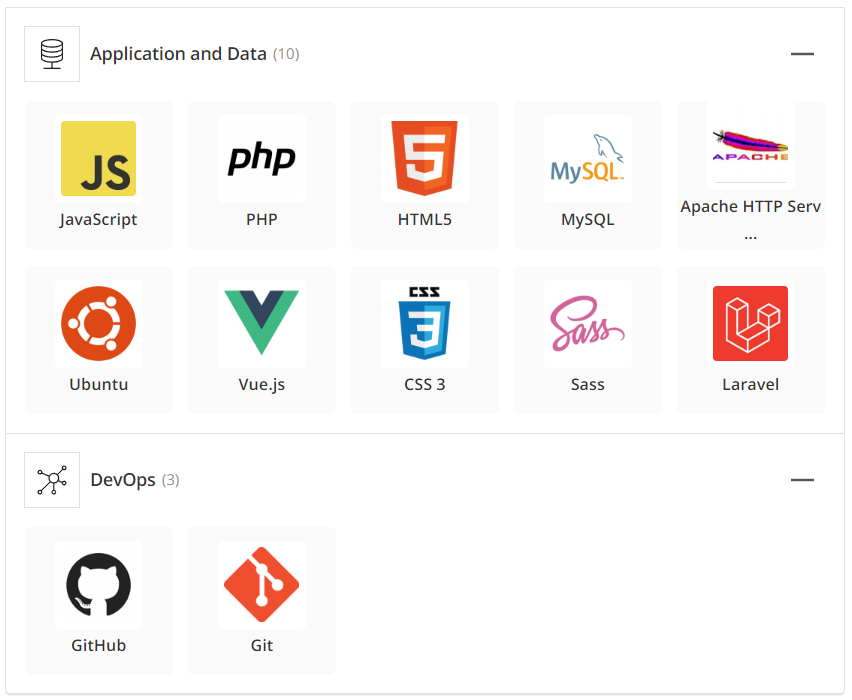
\includegraphics[width=\textwidth]{./assets/figures/stack-old-tb.png}
        \caption[Stack de technologies]{Stack de technologies utilisées via
            \href{https://stackshare.io/alecberney/bachelors-thesis}{stackshare} \label{stack-old-tb}}
    \end{figure}
\end{center}

\subsection{Besoins pour le projet}
Je vais ici définir les besoins du projet et ceci en les séparant par parties distinctes.

\subsubsection{Besoins pour l'infrastructure de développement}
Pour commencer, définissons l'infrastructure de développement.\\
L'infrastructure de développement englobe tous les outils à installer et toutes les configurations à réaliser sur un pc vierge afin que le développeur puisse commencer à développer l'application.
En général, ce qui est recherché, c'est la simplicité et la rapidité de configuration de cet environnement.\\
Dans notre cas, pour que le développeur puisse commencer à développer, il doit principalement mettre en place les outils suivants:
\begin{itemize}
    \item un \Gls{ide} (Integrated Development Environment), de préférence Visual Studio Code,
    \item l'outil de versioning \Gls{git},
    \item un \Gls{sgbd} (Système de Gestion de Base de Données),
    \item le language PHP,
    \item l'outil Composer,
    \item le framework Laravel,
    \item l'environement d'exécution (runtime environment) Node.js,
    \item le framework Vue.js.
\end{itemize}
Comme vous pouvez le voir, la liste devient vite longue et certains des outils à installer prennent passablement de temps et possèdent des configuration spécifiques.\\
Je parle notamment des outils suivants:
\begin{itemize}
    \item le SGBD (Système de Gestion de Base de Données),
    \item le language PHP, avec Composer et le framework Laravel,
    \item l'environement d'exécution (runtime environment) Node.js et le framework Vue.js.
\end{itemize}
Ces outils n'étant pas triviaux à mettre en place et changeant pour chaque projet, il est préférable de simplifier le plus possible leur installation et configuration.

Comme vous l'aurez compris, un des besoins le plus important pour le choix de cette infrastructure, est la simplicité de mise en place du projet.\\
Il faut que cela soit facile à prendre en main et bien documenté.\\
Un des autres points à prendre en compte, est la disponibilité des outils utilisés, dans le sens où des outils payants ne pourraient pas être accessibles pour certains développeur.\\
Créer quelque chose de simple à prendre en main, c'est important, mais il faut aussi prendre en compte la difficulté nécessaire pour mettre en place les outils facilitant la prise en main, par exemple Docker.

\subsubsection{Besoins pour l'infrastructure de production}
Nous allons maintenant faire de même pour l'infrastructure de production.\\
L'infrastructure de production englobe tous les outils à installer et toutes les configurations à réaliser sur un pc vierge afin que le programme final soit accessible est utilisable par n'importe quel utilisateur.\\
En général, la simplicité de mise à jour du programme, la performance et la robustesse sont recherchés.\\
On peut aussi prendre en compte la flexibilité de la solution, dans le sens où il serait facile de déployer le programme final sur une autre machine de production.\\
En effet, la première étape de configuration se réalise peu de fois et si cette dernière est un peu plus compliquée, cela n'est pas forcément un énorme désavantage.\\
Dans notre cas, pour que le programme puisse fonctionner sur le serveur de production, il est nécessaire d'installer tous les outils suivants:
\begin{itemize}
    \item potentiellement l'outil de versioning Git,
    \item un SGBD (Système de Gestion de Base de Données),
    \item le language PHP,
    \item l'outil Composer,
    \item le framework Laravel,
    \item Un serveur \Gls{apache},
    \item Un \Gls{proxy}.
\end{itemize}
La liste des outils à installer et configurer, comme pour l'environnement de développement, est conséquente.\\
Certains outils prennent passablement de temps et possèdent des configuration spécifique.\\
Je parle notamment des outils suivants:
\begin{itemize}
    \item le SGBD (Système de Gestion de Base de Données),
    \item le language PHP, avec Composer et le framework Laravel.
\end{itemize}
Comme expliqué précédemment, une certaine flexibilité et simplicité est recherchée lors de la mise en place de l'infrastructure et c'est pour cela qu'il est préférable de simplifier le plus possible l'installation et la configuration des outils cités ci-dessus.

Si nous résumons les critères qui influenceront notre décision, nous pouvons ressortir ces derniers:
\begin{itemize}
    \item la performance de l'infrastructure,
    \item la simplicité de mise à jour du programme au sein de l'infrastructure,
    \item la robustesse de l'infrastructure,
    \item la flexibilité de l'infrastructure.
\end{itemize}

\subsubsection{Besoins pour les Devops}
Pour finir, nous allons maintenant faire de même pour le pipeline \Gls{devops}.
Le pipeline \Gls{devops} défini toutes les étapes réalisées et les outils utilisé pour parvenir à mettre en place une infrastructure de travail et de livraison de produit fonctionnel et automatisée au maximum.\\
Le but des \Gls{devops} étant d'automatisé le plus de tâches possibles, on attend donc du pipeline les critères suivants:
\begin{itemize}
    \item la performance de l'infrastructure (dans le sens de la rapidité),
    \item la "simplicité" de mise en place du pipeline,
    \item la simplicité de mise à jour du pipeline via une flexibilité maximum,
    \item la robustesse du pipeline,
    \item la possibilité d'ajouter des étapes intermédiaires de tests du produit entre l'infrastructure de développement et de prodution.
\end{itemize}

La flexibilité et simplicité ressort encore une fois dans les besoins de cette section.
Mais un point important est la possibilité de tester manuellement son produit avant de le livrer en production.

\subsubsection{Importance de l'open source et de la gratuité des outils}
Pour tous les choix technologiques qui vont être réaliser, un besoin essentiel intervient.
Plus nous utilisons d'outils open source ou gratuit, plus nous faciliterons l'intégration de n'importe quel développeur au projet.\\
Mais utiliser des outils qui sont gratuits ou open source offre également un plus pour l'intégration aux DevOps car il facilitera de façon non négligeable la mise en place de ces derniers.

% docker
\subsection{Introduction à Docker}
Pour pour pouvoir comparer les différentes infrastructures et faire des choix sur ces dernières, il est important d'introduire l'outil \Gls{docker}.\\
Docker est un outil permettant de gérer des conteneurs.\\
Qu'est-ce qu'un conteneur? Un \Gls{conteneur} est une sorte de machine virtuelle plus légère ayant pour but d'encapsuler une ou plusieurs applications / outils technologiques ainsi que toutes les dépendances que ces applications exigent pour leur bon fonctionnement.\\
Il ne s'agit donc pas de virtualisation mais de "conteneurisation" ou "containerization" en anglais.
Dans une "conteneurisation", seul l'\Gls{os} et le software est virtualisé et non le hardware.\\
Nous remarquons bien la différence avec la figure suivante \ref{docker-compare}

\begin{center}
    \begin{figure}
        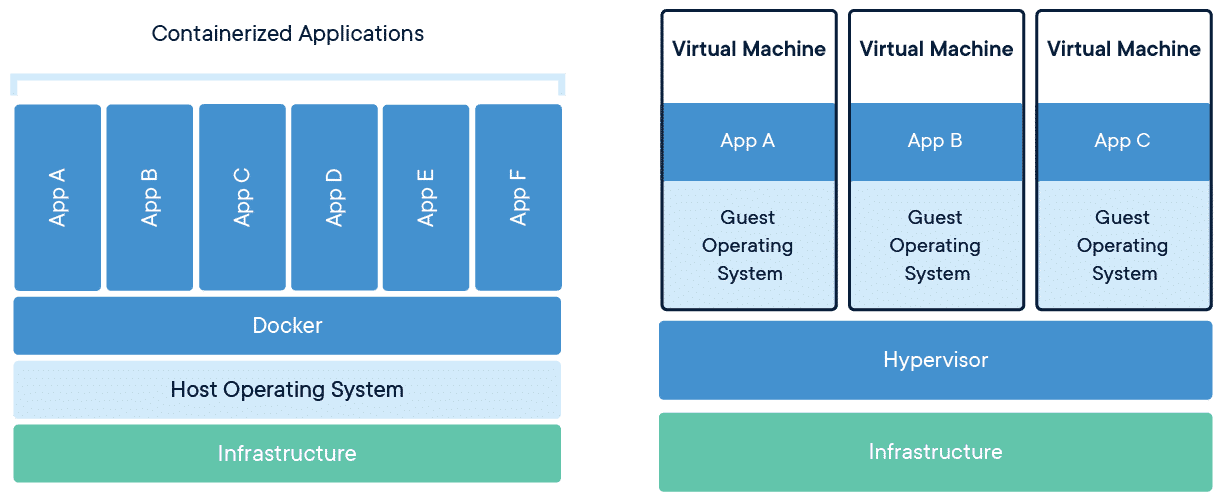
\includegraphics[width=\textwidth]{./assets/figures/docker-containerized-and-vm.png}
        \caption[Comparaison Docker vs VM]{Comparaison entre containeurs docker et machines virtuelles
            du \href{https://www.docker.com/wp-content/uploads/2021/11/}{site docker}
            \label{docker-compare}}
    \end{figure}
\end{center}

Les containers sont facilement téléchargeables et transmissibles. Ils sont également relativement facile à mettre en place.\\
Le principe est simple, nous avons une application et une certaine configuration qui fonctionne, nous pouvons facilement l'encapsuler dans un conteneur et le transmettre à nos collègues ou le télécharger sur un autre pc.\\
Un des principals avantages, est le fait que le conteneur ne dépend pas de l'OS ou de l'état de la machine sur lequel il va être lancé.\\
Le seul point requis, est de posséder docker sur la machine.\\
Cette solution rend plus flexible et portable l'exécution d'application sur n'importe quelle machine.\\
Voici un schéma démontrant la façon dont docker et des conteneurs dockers sont mis en place sur une
machine comme illustré sur la figure \ref{docker-container-app}.

\begin{center}
    \begin{figure}
        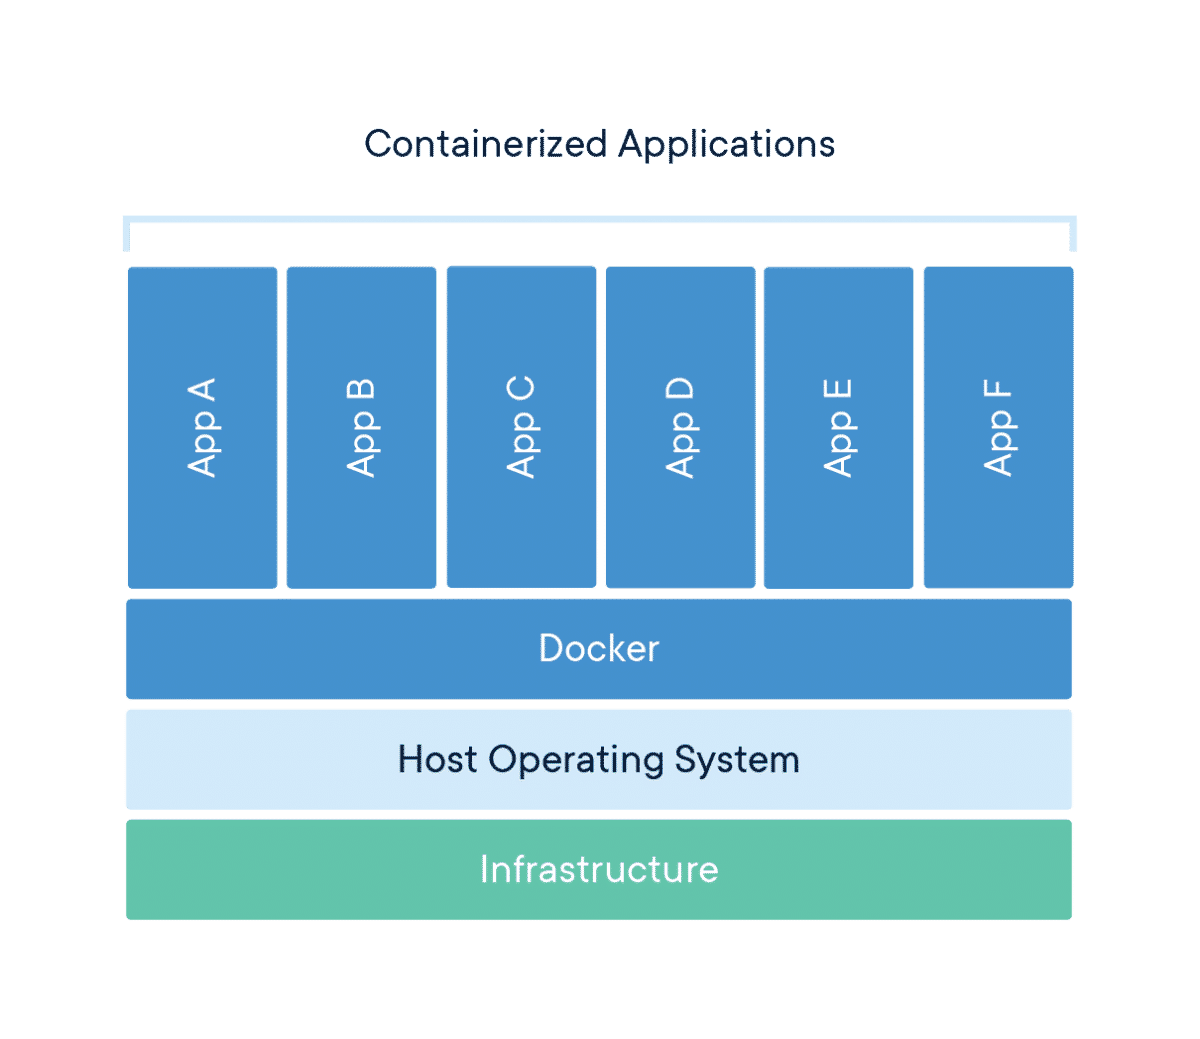
\includegraphics[width=\textwidth]{./assets/figures/container-what-is-container.png}
        \caption[Conteneurisation d'applications]{Conteneurisation d'applications via
            le \href{https://www.docker.com/wp-content/uploads/2021/11/container-what-is-container.png}{site docker}
            \label{docker-container-app}}
    \end{figure}
\end{center}

%https://www.docker.com/resources/what-container/
%https://www.ibm.com/fr-fr/cloud/learn/docker
%https://fr.wikipedia.org/wiki/Docker_(logiciel)
%https://www.youtube.com/watch?v=Gjnup-PuquQ

Voici une liste des avantages généraux de Docker comparé à une VM:
\begin{itemize}
    \item \char"2295 Les conteneurs sont petits comparé au VM \cite{koukia,nick}, %\char{2713}
    \item \char"2295 Les conteneurs utilisent moins de ressources \cite{koukia},
    \item \char"2295 Les conteneurs démarrent plus rapidement \cite{koukia},
    \item \char"2295 Fonctionne bien avec les DevOps et les CI/CD \cite{koukia,data-flair-pros-cons,data-flair-use-cases},
    \item \char"2295 Facilite l'extensibilité horizontale \cite{data-flair-use-cases},
    \item \char"2295 Regroupe les applications et les fichiers système en une seule image standardisée \cite{kane2018docker},
    \item \char"2295 Permet de tester et livrer l'exact même artefact à tous les systèmes et dans tous les
          environnements \cite{kane2018docker,nick},
    \item \char"2295 Créer une abstraction autour de l'application sans sacrifier trop de ressources \cite{kane2018docker}.
\end{itemize}

Voici une liste des inconvénients de Docker comparé à une VM:
\begin{itemize}
    \item \char"2296 La sécurité, \cite{koukia}
    \item \char"2296 L'isolation non complète', \cite{koukia}
    \item \char"2296 La gestion du réseau. \cite{koukia}
\end{itemize}

Pour terminer, on peut voir sur la figure \ref{docker-use-cases} une liste des cas d'utilisations de docker \cite{data-flair-use-cases}.

\begin{center}
    \begin{figure}
        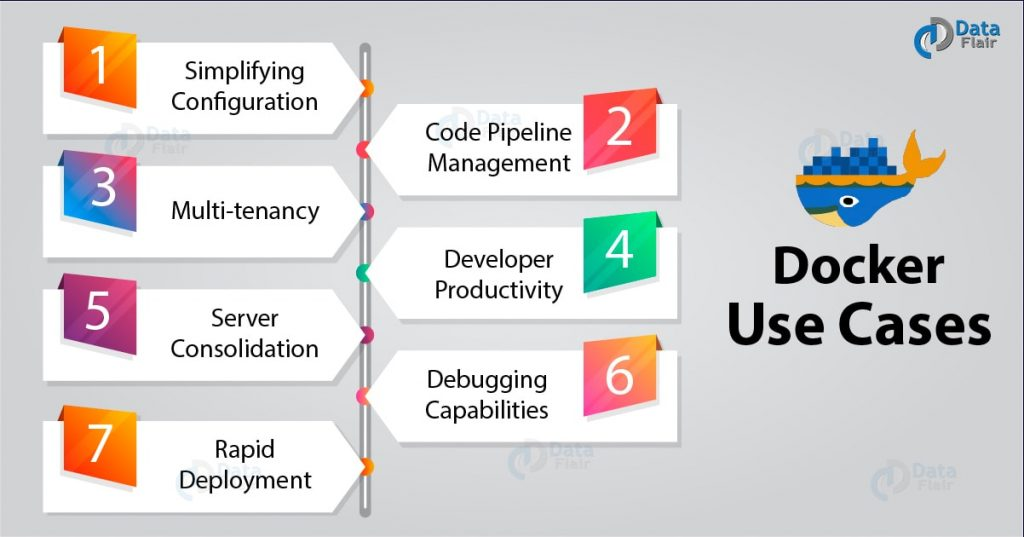
\includegraphics[width=\textwidth]{./assets/figures/docker-use-cases.jpg}
        \caption[Cas d'utilisation de docker]{Cas d'utilisation de docker via \href{https://data-flair.training/blogs/wp-content/uploads/sites/2/2018/10/}{data falir}
            \label{docker-use-cases}}
    \end{figure}
\end{center}

\subsubsection{Docker point de vue sécurité}
En ce qui concerne la sécurité de Docker, je ne me suis pas assez plongé dedans pour ressortir une
analyse concrète et fiable mais j'ai trouvé un article \cite{combe} qui en parle et qui pourrait
être une première direction pour approfondir le sujet.

% Packaging software in a way that leverages the skills developers already have. \cite{kane2018docker}
% Bundling application software and required OS filesystems together in a single standar‐dized image format. \cite{kane2018docker}
% Using packaged artifacts to test and deliver the exact same artifact to all systems in all environments. \cite{kane2018docker}
% Abstracting software applications from the hardware without sacrificing resources \cite{kane2018docker}

% quand ne pas utiliser docker: Performance is critical to your application

%virtual machine vs containers:
%https://www.youtube.com/watch?v=cjXI-yxqGTI
%https://www.ibm.com/cloud/learn/containers?utm_medium=OSocial&utm_source=Youtube&utm_content=000023UA&utm_term=10010608&utm_id=YTDescription-101-Containers-vs-VMs-LH-Containers-Guide&cm_mmc=OSocial_Youtube-_-Cloud+and+Data+Platform_SFT+Cloud+Platform+Digital-_-WW_WW-_-YTDescription-101-Containers-vs-VMs-LH-Containers-Guide&cm_mmca1=000023UA&cm_mmca2=10010608
%https://www.ibm.com/cloud/learn/virtual-machines?utm_medium=OSocial&utm_source=Youtube&utm_content=000005UJ&utm_term=10002434&utm_id=YTDescription-101-Containers-vs-VMs-LH-Virtual-Machines-Guide&cm_mmc=OSocial_Youtube-_-Cloud+and+Data+Platform_PLT+Cloud+Platform+F2F-_-WW_WW-_-YTDescription-101-Containers-vs-VMs-LH-Virtual-Machines-Guide&cm_mmca1=000005UJ&cm_mmca2=10002434


\subsubsection{Performances de Docker}
Docker est outil qui paraît très pratique, mais qu'en est-il de ses performances?
Pour ceci, nous allons retracer quelques évalutations réalisées lors d'une étude de IBM. Nous allons parcourir ces évalutations via des graphiques, tiré de l'étude, résumants bien les résultats.
Commençant par la latence que peut apporter Docker indiquée sur la figure \ref{network-latency}.

\begin{center}
    \begin{figure}
        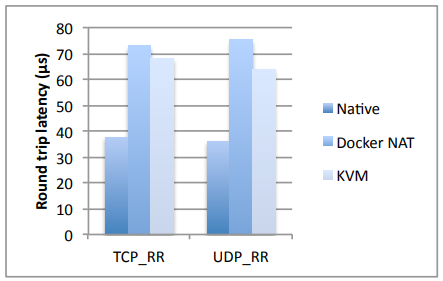
\includegraphics[width=\textwidth]{./assets/figures/docker-perf-latency.png}
        \caption[Docker latence aller-retour du réseau]{Latence aller-retour du réseau (µs) \cite{rad2017introduction} \label{network-latency}}
    \end{figure}
\end{center}

On constate que la latence double, mais nous parlons ici de microsecondes, et de 30 microsecondes supplémentaires, ce qui est en soit assez peu pour de petite infrastructure.

En ce qui concerne le transfert de grosses quantité de données via \gls{tcp}, docker parvient à se
rapprocher des performances d'une machine native, elles n'utilisent donc pas beaucoup plus de cycles
comme illustré dans la figure \ref{tcp-transfer-latency}.

\begin{center}
    \begin{figure}
        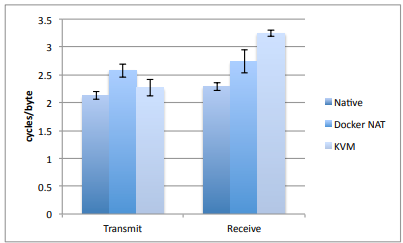
\includegraphics[width=\textwidth]{./assets/figures/docker-perf-transfer-efficiancy.png}
        \caption[Docker efficacité du transfert de masse]{Efficacité du transfert de masse TCP (cycles CPU/octet) \cite{rad2017introduction} \label{tcp-transfer-latency}}
    \end{figure}
\end{center}

Au niveau des écritures, on remarque grâce aux deux graphiques suivants que les performances valent
celles d'un système natif comme le montre les figures \ref{sequential-io} et \ref{random-io}

\begin{center}
    \begin{figure}
        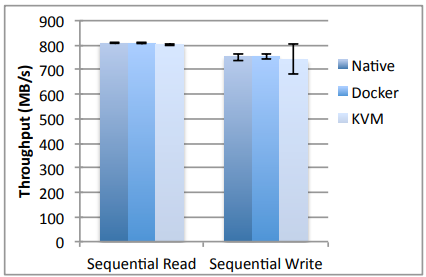
\includegraphics[width=\textwidth]{./assets/figures/docker-perf-sequential-io.png}
        \caption[Docker débit d'I/O séquentielles]{Débit d'Entrée/Sortie séquentielles (Mo/s) \cite{rad2017introduction} \label{sequential-io}}
    \end{figure}
\end{center}

\begin{center}
    \begin{figure}
        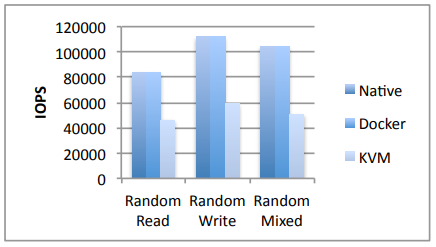
\includegraphics[width=\textwidth]{./assets/figures/docker-perf-random-io.png}
        \caption[Débit d'I/O aléatoires]{Débit d'Entrée/Sortie aléatoires (IOPS) \cite{rad2017introduction} \label{random-io}}
    \end{figure}
\end{center}

On peut également observer sur la figure \ref{docker-perf-mysql} des performances sur le SGBD MySQL
que nous utilisons pour le projet.

\begin{center}
    \begin{figure}
        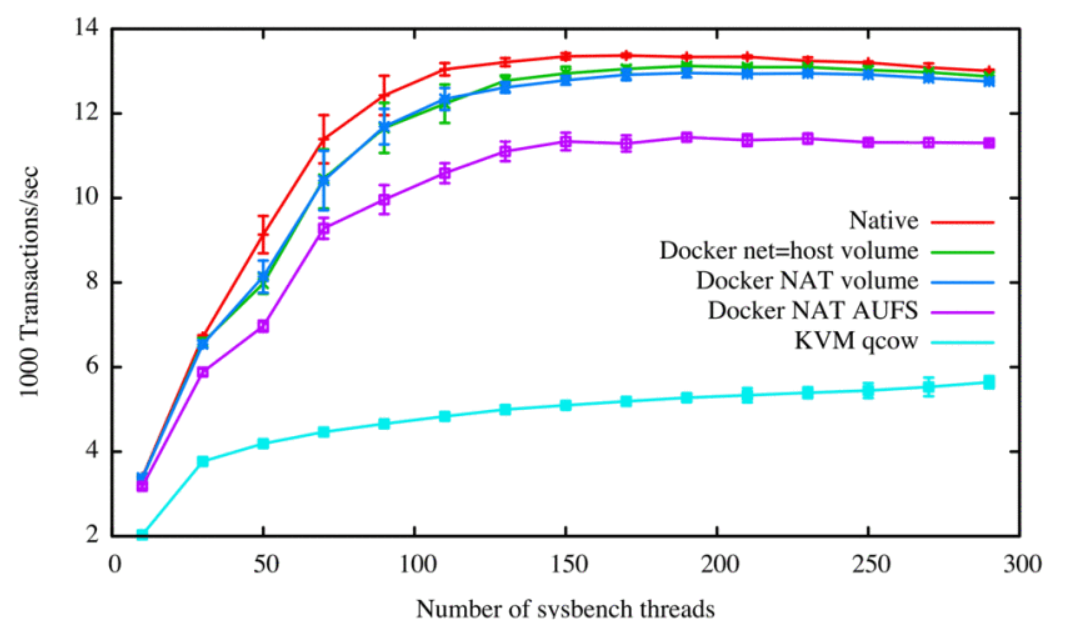
\includegraphics[width=\textwidth]{./assets/figures/docker-perf-mysql.png}
        \caption[Comparaison des perf. Docker sur MySQ]{Comparaison des performances de Docker avec des
            transactions sur MySQL \cite{felter} \label{docker-perf-mysql}}
    \end{figure}
\end{center}

Beaucoup d'autres informations ressortent dans un article étudiant les performances de Docker pour
des applications demandant une grande performance. \cite{chung}
Un point intéressant, qui me paraît important, est celui de la gestion de la mémoire vive qu'utilise
Docker, illustré sur la figure \ref{docker-perf-ram}.\\
On voit clairement que Docker n'est pas pas plus gourmand qu'une machine native et c'est un bon point.

\begin{center}
    \begin{figure}
        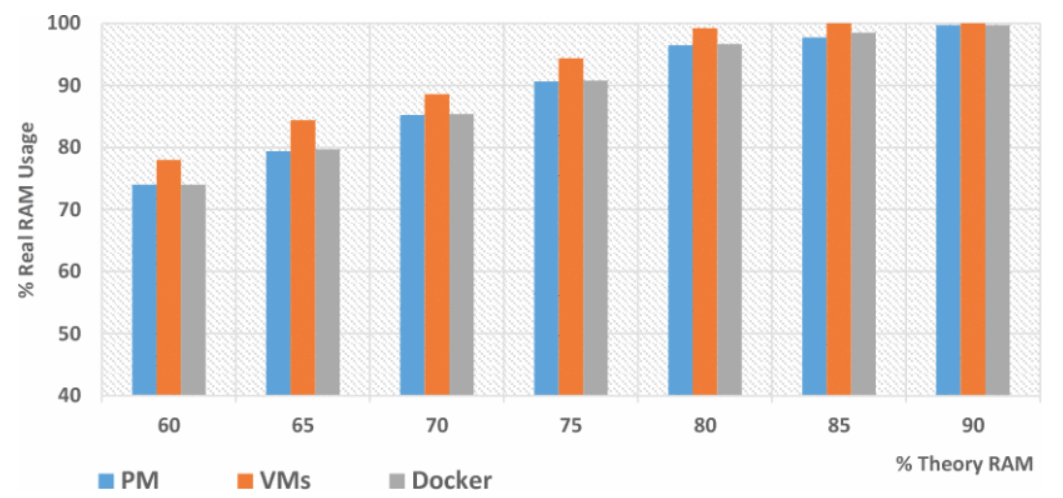
\includegraphics[width=\textwidth]{./assets/figures/docker-perf-ram.png}
        \caption[Comparaison des perf. Docker sur la RAM]{Comparaison des performances de Docker au
            niveau de l'utilisation de la mémoire vive \cite{chung} \label{docker-perf-ram}}
    \end{figure}
\end{center}

%docker en prod perf:
%https://stackoverflow.com/questions/21691540/how-to-optimize-performance-for-a-docker-container/21707838#21707838
%https://stackoverflow.com/questions/21889053/what-is-the-runtime-performance-cost-of-a-docker-container
%https://dominoweb.draco.res.ibm.com/reports/rc25482.pdf
%https://www.freecodecamp.org/news/7-cases-when-not-to-use-docker/

\subsubsection{Et Kubernetes?}
Pourquoi utiliserions-nous forcément docker sans avoir réfléchi à la possibilité de \Gls{kubernetes}?
Pour commencer, comme indiquer sur le site officiel:
"Kubernetes est un système open-source permettant d'automatiser le déploiement, la mise à l'échelle et la gestion des applications conteneurisées".\\
Kubernetes n'est donc pas vraiment une alternative à docker, mais peut être plutôt utiliser comme complément à ce dernier.\\
Comme la partie principale de Kubernetes est de gérer les applications conteneurisées et de simplifier le load balancing, par exemple, il n'est pas forcément utile pour nous d'approfondir les recherches sur le sujet.\\
En effet, La charge attendu par l'application déployée ne devrait pas dépasser les 100 utilisateurs simultanés. La question du load-balancing est donc écartée, tout comme la mise en place d'un cluster Kubernetes.

% comment mettre en place -> voir avec monsieur Graf / regarder avec des profs
% si question pointu, peuvent être transférer à m. chevallier

%https://kubernetes.io/
%https://www.youtube.com/watch?v=PziYflu8cB8
%docker vs k8s, IBM: https://www.youtube.com/watch?v=2vMEQ5zs1ko
%https://www.ibm.com/cloud/learn/kubernetes?cm_mmc=OSocial_Youtube-_-Hybrid+Cloud_Cloud+Platform+Digital-_-WW_WW-_-KubevsDockerYTDescription&cm_mmca1=000023UA&cm_mmca2=10010608#toc-what-is-ku-nVcfWlWE

%https://stackshare.io/: outil très utile pour faire des comparaisons de technologies

\subsubsection{Autres solutions de conteneurs}
Une question se pose, pourquoi utiliserions-nous forcément Docker alors que d'autres solutions existent?
Pour commencer, voici une liste non exhaustive des solutions alternatives à Docker:
\begin{itemize}
    \item \href{https://fr.wikipedia.org/wiki/BSD_Jail}{BSD Jails},
    \item \href{https://linuxcontainers.org/lxd/}{LXD},
    \item \href{https://linuxcontainers.org/lxc/introduction/}{LXC},
    \item \href{https://docs.oracle.com/cd/E18440_01/doc.111/e18415/chapter_zones.htm#OPCUG426}{Solaris Zones},
    \item \href{https://www.redhat.com/en/topics/containers/what-is-rkt}{RKT}.
\end{itemize}

Le principal problème de ces solutions est le manque de popularité comme on peut le remarquer sur la
figure \ref{containers-trends} représentant les recherches concernant les différents sujets via l'outil \href{https://trends.google.fr/trends}{Google trends}.\\
Le fait de ne pas être populaire est un gros désavantage pour ces solutions car très peu d'informations, de tutoriels et de documentations sont disponibles sur internet.\\
Ce simple fait suffit à orienté le choix de la solution de conteneur sur Docker.\\
N'ayant également pas le temps d'analyser chaque solution en profondeur dans ce travail, cela conforte mon choix.

\begin{center}
    \begin{figure}
        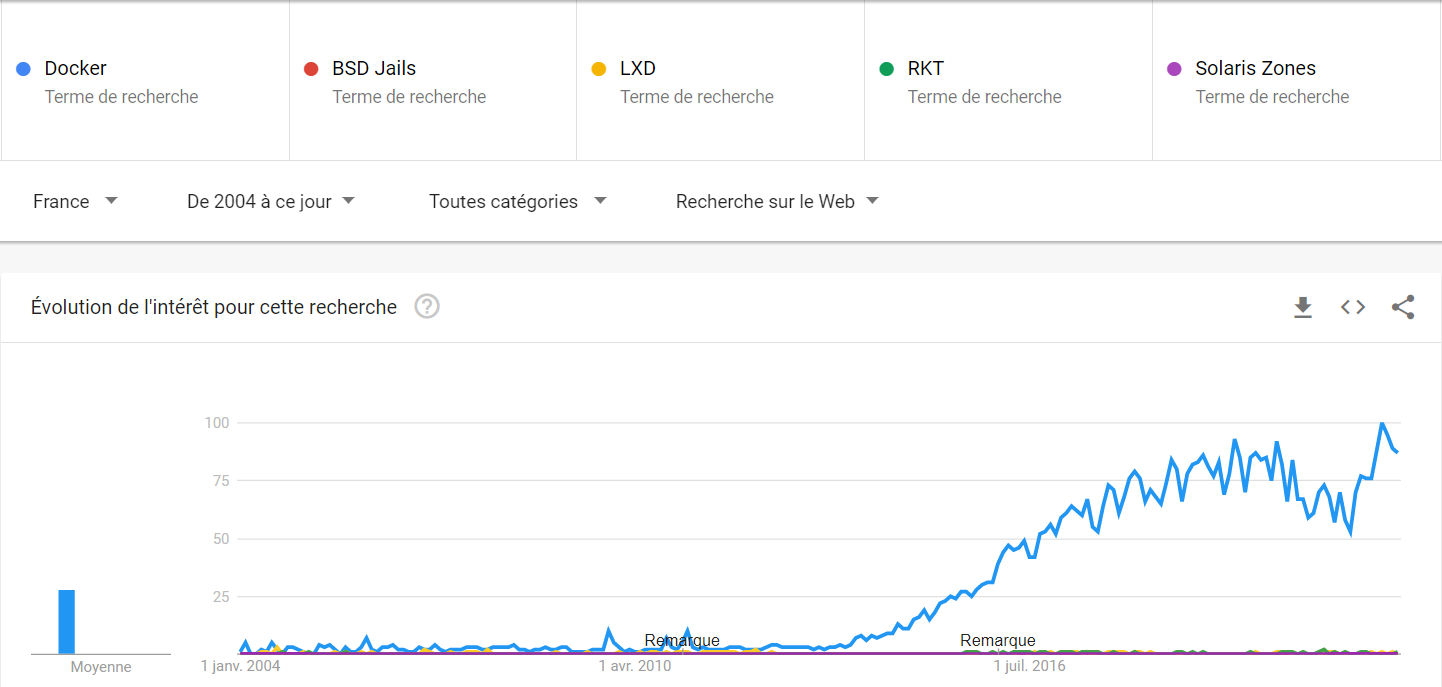
\includegraphics[width=\textwidth]{./assets/figures/google-trend-containers-2022.png}
        \caption[Tendances solutions de conteneurs]{Tendances sur les différentes solutions de conteneurs depuis 2004} \label{containers-trends}
    \end{figure}
\end{center}

% dev
\subsection{Infrastructures de développement}

\subsubsection{Présentation des infrastructures de développement possibles}

%\figi{infrastructure-dev-choix.drawio}{18cm}{Différentes possibilités d'infrastructure de développement}

L'infrastructure que vous pouvez voir dans la figure \ref{infrastructure-dev-actuelle.drawio} et celle qui était utilisée lorsque j'ai reprise le projet.\\
En résumé, tous les outils ont été installés nativement sur la machine de développement sans virtualisation.
%\figi[Infra. dev. actuelle]{infrastructure-dev-actuelle.drawio}{18cm}{Infrastructure de développement actuelle}

Ensuite, nous avons la possibilité d'utiliser une infrastructure avec uniquement la base de données
en conteneur Docker, comme illustré sur la figure \ref{infrastructure-dev-db-laravel-docker.drawio}.
%\figi[Infra. dev. avec DB en Docker]{infrastructure-dev-db-docker.drawio}{16cm}{Infrastructure de développement avec une DB en Docker}

Comme nouveau changement, il est également possible de passer tout l'environnement de développement
du Backend sous plusieurs conteneurs Docker en utilisant un outil fourni par Laravel, \href{https://laravel.com/docs/9.x/sail}{Sail}.
%\figi[Infra. dev. avec DB + Laravel en Docker]{infrastructure-dev-db-laravel-docker.drawio}{16cm}{Infrastructure de développement avec une DB et Laravel en Docker}

Une autre possibilité du même genre étant Laravel
\href{https://laravel.com/docs/9.x/homestead}{Homestead} qui est un environnement de développement
virtualisé à l'aide d'une machine virtuelle \href{https://www.vagrantup.com/}{Vagrant}.\\
Cette solution est considérée comme le prédecesseur à Laravel Sail qui est beaucoup plus léger.\\
C'est pourquoi, cette solution ne fera pas parti des choix que nous allons argumenter, mais est
présentée comme complément. Cette solution correspond à la figure \ref{infrastructure-dev-laravel-homestead.drawio}.
%\figi[Infra. dev. avec Homestead]{infrastructure-dev-laravel-homestead.drawio}{16cm}{Infrastructure de développement avec Laravel Homestead}

Finalement, une infrastructure avec tous les projets en conteneurs Docker est possible et visible
avec la figure \ref{infrastructure-dev-db-laravel-vuejs-docker.drawio}.
%\figi[Infra. dev. avec DB + Laravel + Vue en Docker]{infrastructure-dev-db-laravel-vuejs-docker.drawio}{16cm}{Infrastructure de développement avec une DB, Laravel et Vue.js en Docker}

%https://laravel.com/docs/9.x/sail
%https://blog.logrocket.com/laravel-and-docker-a-guide-to-using-laravel-sail/
%https://r00t4bl3.com/post/how-to-setup-docker-environment-for-laravel-development
%https://dockerize.io/guides/php-laravel-guide
%https://www.honeybadger.io/blog/laravel-docker-php/

\clearpage

\subsubsection{Évolutions de l'infrastructure de développement possibles}
Les différentes infrastructures désormais présentées, il est nécessaire de les comparer en listant les pours et les contres de chaque changement en prenant comme référentielle l'infrastructure actuelle.\\
Les 3 améliorations (combinées ou non) proposées sont les suivantes:
\begin{itemize}
    \item Passage du SGBD en machine Docker,
    \item Passage du projet Laravel (et toutes ces technologies) en machine Docker,
    \item Passage du projet Vue.js (et toutes ces technologies) en machine Docker.
\end{itemize}

\subsubsection{Passage du SGBD en conteneur Docker}
Commençons par réfléchir sur le passage du SGBD en conteneur Docker.
% vraiment bien se blinder au niveau des arguments via blog et études, sources écrites
% si on a pas trouvé, on peut dire je ne sais pas, on DOIT dire -> joker ultime
% toucher quelque chose en surface, si je ne connais pas, si point essentiel dans projet, faire un choix + essai -> prototype, démonstration sur expérience
% aussi parlé des charges qui devront être supportées et si c'est possible, nb user final par ex
Pour ceci, nous allons énumérer les avantages et inconvénients d'installer le SGBD nativement.
Ces derniers sont visible avec la table \ref{dev-sgbd-native}

\begin{table}[h]
    \begin{center}
        \caption{SGBD natif \label{dev-sgbd-native}}
        \begin{tabularx}{1.0\textwidth} {X|X}
            Avantages                                                                    & Inconvénients \\ \hline
            \char"2295 Gestion de la BD plus facile car le SGBD est installé nativement  &
            \char"2296 Demande du temps pour l'installation                                              \\
            \char"2295 Le SGBD peut-être déjà installé et peut être utilisée directement &
            \char"2296 Configuration à réaliser à la main                                                \\
            \char"2295 Ne nécessite pas Docker                                           &
            \char"2296 Fort
            risque d'erreur lors de la configuration                                                     \\             & \char"2296 Installation
            différente pour chaque OS                                                                    \\
        \end{tabularx}
    \end{center}
\end{table}

Nous allons, maintenant, énumérer les avantages et inconvénients d'avoir le SGBD en conteneur
Docker. Ces derniers sont visible avec la table \ref{dev-sgbd-docker}

\begin{table}[h]
    \begin{center}
        \caption{SGBD en conteneur Docker \label{dev-sgbd-docker}}
        \begin{tabularx}{1.0\textwidth} {X|X}
            Avantages                             & Inconvénients                                                         \\ \hline
            Accélère l'installation de l'environnement de développement,
            \cite{labrecque,data-flair-pros-cons} & Gestion de la BD
            potentiellement plus compliquée                                                                               \\
            Apporte de la cohérence au niveau des technologies utilisées, au sein de l'équipe,
            \cite{labrecque,data-flair-use-cases} & Docker peut avoir des problèmes de performances,
            \cite{labrecque}                                                                                              \\
            Rend le debugging dû aux environnements de développement plus facile,
            \cite{labrecque,koukia}               & Nécessite Docker et les connaissances qui vont avec. \cite{labrecque} \\
            Facilite la configuration, car elle est en gande partie déjà réalisée,
            \cite{data-flair-pros-cons}           &                                                                       \\
            Compatible avec tous les OS           &                                                                       \\
        \end{tabularx}
    \end{center}
\end{table}

Si nous évaluons les deux solutions proposées selon les besoins suivants:
\begin{itemize}
    \item simplicité de mise en place du projet,
    \item la disponibilité des outils utilisés,
    \item la difficulté nécessaire pour mettre en place les outils facilitant la prise en main.
\end{itemize}

On se rend facilement compte que la solution avec Docker est celle qui se rapproche le plus de ces derniers.

\subsubsection{Passage de Laravel en conteneur Docker}
Passons maintenant au passage de l'environnement Laravel en conteneur Docker.\\
Pour ceci, nous allons énumérer les avantages et inconvénients d'installer nativement cet
environnement. Ces derniers sont visible avec la table \ref{dev-laravel-native}.

\begin{table}[h]
    \begin{center}
        \caption{Laravel natif \label{dev-laravel-native}}
        \begin{tabularx}{1.0\textwidth} {X|X}
            Avantages                         & Inconvénients
            \\ \hline
            (Meilleur performance)            & Peut générer des conflits si plusieurs versions sont présentes \\
            Gestion totale de l'environnement & Impossibilité d'avoir plusieurs versions différentes
            installées                                                                                         \\
                                              & L'installation demande du temps                                \\
                                              & Configuration à faire à la main                                \\
                                              & Fort risque d'erreur lors de la configuration                  \\
                                              & Installation différente pour chaque OS                         \\
        \end{tabularx}
    \end{center}
\end{table}

Nous allons, maintenant, énumérer les avantages et inconvénients d'avoir l'environnement Laravel en
machine Docker. Ces derniers sont visible avec la table \ref{dev-laravel-docker}.

\begin{table}[h]
    \begin{center}
        \caption{Laravel en conteneur Docker \label{dev-laravel-docker}}
        \begin{tabularx}{1.0\textwidth} {X|X}
            Avantages                                                                                                                 & Inconvénients
            \\ \hline
            Accélère l'installation de l'environnement de développement, \cite{labrecque}                                             &                                                                         \\
            Apporte de la cohérence au niveau des technologies utilisées, au sein de l'équipe, \cite{labrecque, data-flair-use-cases} & \Gls{docker} peut avoir des problèmes de performances, \cite{labrecque} \\
            Rend le debugging dû aux environnements de développement plus facile, \cite{labrecque,koukia}                             & Nécessite Docker et les connaissances qui vont avec. \cite{labrecque}   \\
            Facilite la configuration, car elle est en gande partie déjà réalisée, \cite{data-flair-pros-cons}                        &                                                                         \\
            Compatible avec tous les OS                                                                                               &                                                                         \\
            Existance d'un outil donné par Laravel et conçu pour être utiliser avec \Gls{docker}, il
            s'agit de \href{https://laravel.com/docs/9.x/sail}{Sail}
                                                                                                                                      &                                                                         \\
            Permet d'avoir plusieurs versions installées                                                                              &                                                                         \\
        \end{tabularx}
    \end{center}
\end{table}

Si nous évaluons les deux solutions proposées selon les besoins suivants:
\begin{itemize}
    \item simplicité de mise en place du projet,
    \item la disponibilité des outils utilisés,
    \item la difficulté nécessaire pour mettre en place les outils facilitant la prise en main.
\end{itemize}

On se rend facilement compte que la solution avec Laravel Sail est celle qui se rapproche le plus de ces derniers. Et que encore une fois, la solution contenant du Docker paraît assez adaptée.

%https://laravel.com/docs/9.x/sail
%https://laravel.com/docs/9.x/homestead

\subsubsection{Passage de Vue.js en conteneur Docker}
Finalement, parlons du passage de l'environnement \Gls{vuejs} en conteneur Docker.

Pour ceci, nous allons énumérer les avantages et inconvénients d'installer nativement cet
environnement. Ces derniers sont visible avec la table \ref{dev-vuejs-native}.

\begin{table}[h]
    \begin{center}
        \caption{Vue.js natif \label{dev-vuejs-native}}
        \begin{tabular}{c|c}
            Avantages                                           & Inconvénients                   \\ \hline
            (Meilleur performance)                              & Configuration à faire à la main \\
            \Gls{nodejs} possède un bon gestionnaire de version &                                 \\
            Compatible avec tous les OS                         &                                 \\
            Gestion totale de l'environnement                   &                                 \\
        \end{tabular}
    \end{center}
\end{table}

Nous allons, maintenant, énumérer les avantages et inconvénients d'avoir l'environnement Laravel en
machine Docker.Ces derniers sont visible avec la table \ref{dev-vuejs-docker}.

\begin{table}[h]
    \begin{center}
        \caption{Vue.js en conteneur Docker \label{dev-vuejs-docker}}
        \begin{tabular}{c|c}
            Avantages                                   & Inconvénients                                       \\ \hline
            Rapide à installer                          & Nécessite Docker et les connaissances qui vont avec \\
            Configuration en gande partie déjà réalisée & Peut-être compliqué à mettre en place               \\
            Compatible avec tous les OS                 &                                                     \\
        \end{tabular}
    \end{center}
\end{table}

Si nous évaluons les deux solutions proposées selon les besoins, désormais bien connus et suivants:
\begin{itemize}
    \item simplicité de mise en place du projet,
    \item la disponibilité des outils utilisés,
    \item la difficulté nécessaire pour mettre en place les outils facilitant la prise en main.
\end{itemize}

On se rend compte que la solution avec Docker n'apporte pas forcément assez d'avanatages comparé à
celle proposant l'installation native et cela est principalement dû au bon gestionnaire de paquets
\href{https://www.npmjs.com/}{NPM} de Javascript. C'est pourquoi, la solution proposant
l'installation native sera préférée.

\subsubsection{Résultat de l'analyse}
Suite à cette analyse des outils, la solution la plus adaptée semble être de mettre en place
l'environement de développment illustré sur le tableau \ref{env-dev}.

\begin{table}[h]
    \begin{center}
        \caption{Environement de développment choisi \label{env-dev}}
        \begin{tabular}{c|c}
            Outil             & Technologie utilisée             \\ \hline
            SGBD - MySQL      & Docker (inclu dans Laravel Sail) \\
            Frontend - Vue.js & Installation native              \\
            Backend - Laravel & Laravel Sail (Docker)            \\
        \end{tabular}
    \end{center}
\end{table}

Finalement cela correspond à la figure numéro \ref{infrastructure-dev-db-laravel-docker.drawio}.

% prod
\clearpage
\subsection{Infrastructures de production}

\subsubsection{Présentation des infrastructures de production possibles}

%\figi{infrastructure-prod-choix.drawio}{16cm}{Différentes possibilités d'infrastructure de production}

L'infrastructure de production que vous pouvez voir dans la figure \ref{infrastructure-prod-actuelle.drawio} et celle qui était utilisée lorsque j'ai reprise le projet.\\
En résumé, tous les outils ont été installés nativement sur la machine de production sans virtualisation.\\
%\figi{infrastructure-prod-actuelle.drawio}{16cm}{Infrastructure de production actuelle}

La figure \ref{infrastructure-prod-db-docker.drawio}, montre la première amélioration possible, c'est à dire, de passer le SGBD en conteneur docker.
%\figi{infrastructure-prod-db-docker.drawio}{16cm}{Infrastructure de production avec une db en docker}

La figure \ref{infrastructure-prod-db-laravel-docker.drawio}, montre la seconde amélioration possible (mais aussi la première), c'est à dire, de passer l'application web réalisée avec le framework Laravel en conteneur docker.
%\figi{infrastructure-prod-db-laravel-docker.drawio}{16cm}{Infrastructure de production avec une db et laravel en docker}

\subsubsection{Évolutions de l'infrastructure de production possibles}
Les différentes infrastructures possibles désormais présentées, il est nécessaire de les comparer en listant les pours et les contres de chaque changement en prenant comme référentielle l'infrastructure actuelle.\\
Les deux améliorations (combinées ou non) proposées sont les suivantes:
\begin{itemize}
    \item Passage du SGBD en machine Docker,
    \item Passage du projet Laravel (et toutes ces technologies) en machine Docker.
\end{itemize}

\subsubsection{Passage du SGBD en conteneur Docker}
Nous recommençons également par réfléchir sur le passage du SGBD en machine Docker.

Pour ceci, nous allons énumérer les avantages et inconvénients d'installer le SGBD nativement.
Certains peuvent être les mêmes qu'énumérer dans la partie "Infrastructure de
développement". Ces derniers sont visible avec la table \ref{prod-db-native}.

\begin{table}[h]
    \begin{center}
        \caption{SGBD natif \label{prod-db-native}}
        \begin{tabularx}{1.0\textwidth} {X|X}
            Avantages                                                         & Inconvénients                          \\ \hline
            Gestion de la BD plus facile car le SGB est installé nativement   & Demande du temps
            pour l'installation                                                                                        \\
            Sauvegarde aisément réalisable                                    & Configuration à réaliser à la main     \\
            Mise en place d'un service de façon triviale                      &                                        \\
            Le SGBD peut-être déjà installé et peut être utilisée directement & Fort risque
            d'erreur lors de la configuration                                                                          \\
            Ne nécessite pas Docker                                           & Installation différente pour chaque OS \\
        \end{tabularx}
    \end{center}
\end{table}

Nous allons, maintenant, énumérer les avantages et inconvénients d'avoir le SGBD en conteneur
Docker. Ces derniers sont visible avec la table \ref{prod-db-docker}.

\begin{table}[h]
    \begin{center}
        \caption{SGBD en conteneur Docker \label{prod-db-docker}}
        \begin{tabularx}{1.0\textwidth} {X|X}
            Avantages                                                & Inconvénients                                                        \\ \hline
            Accélère l'installation de l'environnement de production & Gestion de la BD
            potentiellement plus compliquée                                                                                                 \\
            Facilite la mise à jour de l'environnement de production si l'environnement de
            développement intègre un containeur docker pour le SGBD  & Sauvegarde de la BD
            potentiellement plus compliquée                                                                                                 \\
            Configuration en gande partie déjà réalisée              & Mise en place d'un service non trivial                               \\
            Compatible avec tous les OS                              & Docker peut avoir des problèmes de performances
            \cite{labrecque}                                                                                                                \\
                                                                     & Nécessite Docker et les connaissances qui vont avec \cite{labrecque} \\
        \end{tabularx}
    \end{center}
\end{table}

Si nous évaluons les deux solutions proposées selon les besoins, désormais bien connus et suivants:
\begin{itemize}
    \item la performance de l'infrastructure,
    \item la simplicité de mise à jour du programme au sein de l'infrastructure,
    \item la robustesse de l'infrastructure,
    \item la flexibilité de l'infrastructure.
\end{itemize}

On se rend compte que les deux solutions se valent à peu de chose près. Je choisi donc d'essayer de mettre en place une infrastructure avec Docker en premier temps. Si cela est trop compliqué, l'autre solution étant viable pourra toujours être utilisée.

\subsubsection{Passage de Laravel en conteneur Docker}
Passons maintenant au passage de l'environnement Laravel en conteneur Docker.

Pour ceci, nous allons énumérer les avantages et inconvénients d'installer nativement cet
environnement. Ces derniers sont visible avec la table \ref{prod-laravel-native}.

\begin{table}[h]
    \begin{center}
        \caption{Laravel natif \label{prod-laravel-native}}
        \begin{tabularx}{1.0\textwidth} {X|X}
            Avantages                         & Inconvénients                                             \\ \hline
            (Meilleur performance)            & Mise à jour compliquée si un changement de version à lieu \\
            Gestion totale de l'environnement & L'installation demande du temps                           \\
                                              & Configuration à faire à la main                           \\
                                              & Fort risque d'erreur lors de la configuration             \\
                                              & Installation différente pour chaque OS                    \\
        \end{tabularx}
    \end{center}
\end{table}

Nous allons, maintenant, énumérer les avantages et inconvénients d'avoir l'environnement Laravel
en machine Docker. Ces derniers sont visible avec la table \ref{prod-laravel-docker}.

\begin{table}[h]
    \begin{center}
        \caption{Laravel en conteneur Docker \label{prod-laravel-docker}}
        \begin{tabularx}{1.0\textwidth} {X|X}
            Avantages                                                & Inconvénients                      \\ \hline
            Mise à jour du programme facilitée, dans tous les cas    & Peut laisser des failles de
            sécurité, suivant l'environnement mis en place                                                \\
            Accélère l'installation de l'environnement de production & Mise en place d'un service
            non trivial                                                                                   \\
            Configuration en gande partie déjà réalisée              & Docker peut avoir des problèmes de
            performances, \cite{labrecque}                                                                \\
            Offre une possibilité d'extensibilité horizontale        & Nécessite Docker et les
            connaissances qui vont avec. \cite{labrecque}                                                 \\
            Compatible avec tous les OS                              &                                    \\
        \end{tabularx}
    \end{center}
\end{table}

Si nous évaluons les deux solutions proposées selon les besoins, désormais bien connus et suivants:
\begin{itemize}
    \item la performance de l'infrastructure,
    \item la simplicité de mise à jour du programme au sein de l'infrastructure,
    \item la robustesse de l'infrastructure,
    \item la flexibilité de l'infrastructure.
\end{itemize}

On se rend compte que la solution avec Docker paraît plus adaptée. Cependant, si cela venait à être est trop compliqué, l'autre solution étant viable pourra toujours être utilisée.

% TODO pour le déploiment, regarder pourquoi certains sont parti de docker

\subsubsection{Résultat de l'analyse}
Suite à cette analyse des outils, la solution la plus adaptée semble être de mettre en place
l'environnement de production suivant \ref{env-prod}.

\begin{table}[h]
    \begin{center}
        \caption{Environement de production choisi \label{env-prod}}
        \begin{tabular}{c|c}
            Outil             & Technologie utilisée \\ \hline
            SGBD - MySQL      & Docker               \\
            Backend - Laravel & Docker               \\
        \end{tabular}
    \end{center}
\end{table}

Finalement cela correspond à la figure numéro \ref{infrastructure-prod-db-laravel-docker.drawio}.

\subsubsection{Analyse de risques}
% comment protéger une infra en prod
% contacter des profs de sécu
% lister ce qu'on va mettre en place
% on est resté en surface, il faudrait investir des experts pour évaluer. (audit par exemple)
% sécurité pas prise en compte dans le projet car pas dans objectif, pas le luxe de rechercher car trop de temps, à mentionner dans le rapport.

L'analyse de risques de l'infrastructure de production est un point très important lorsque l'on publie un logiciel. Cette dernière peut être très complexe et nécessite énormément de connaissances.
Une analyse de risque complète demande une quantité conséquente de travail. L'intervention d'experts dans le domaine, via par exemple, des audits serait une solution pour réaliser cette partie du projet.\\
L'analyse de risques ne pourra donc pas être réaliser lors de ce projet, pour toutes les raisons énumérées plus haut, mais aussi car ce n'est pas le but principal de ce dernier.\\
J'ai donc décider d'appliquer tout ce que je connaissais et faire le meilleur travail possible sans aller en profondeur dans le sujet.

% devops
%https://blog.logrocket.com/how-to-create-a-ci-cd-for-a-laravel-application-using-github-actions/

\clearpage
\subsection{Pipeline DevOps}
\subsubsection{Introduction aux Devops}
%https://www.youtube.com/watch?v=scEDHsr3APg
%https://www.padok.fr/blog/devops-tout-savoir
%https://azure.microsoft.com/en-us/overview/what-is-devops/#devops-overview
%https://www.ibm.com/cloud/learn/devops-a-complete-guide
Pour commencer, c'est quoi les DevOps?\\
Les DevOps c'est un ensemble de processus permettant de gérer et faciliter le développement et le déploiement continu de l'application. Cela permet de garantir une meilleure qualité du code et de simplifier l'intégration de ce dernier. C'est-à-dire, si un collaborateur souhaite ajouter sa partie du code au projet, il doit d'abord passer par un système automatisé de contrôle et d'intégration de son code avant de pouvoir l'ajouter. Cette partie est appelée \Gls{ci}.\\
Les DevOps intègre également tout ce qui est déployement continu et livraison continue (\Gls{cd}).
En pratique, ils intègrent également d'autre aspect, comme la maintenance de l'infrastructure de
production et de développement, la sécurité des processus et beaucoup d'autres concepts.\\
Au final c'est un cycle de vie visant à faciliter le développement d'applications en équipe.\\
On peut observer un exemple de lifecycle fourni par IBM selon la figure \ref{devops-lifecycle}.

\begin{center}
    \begin{figure}
        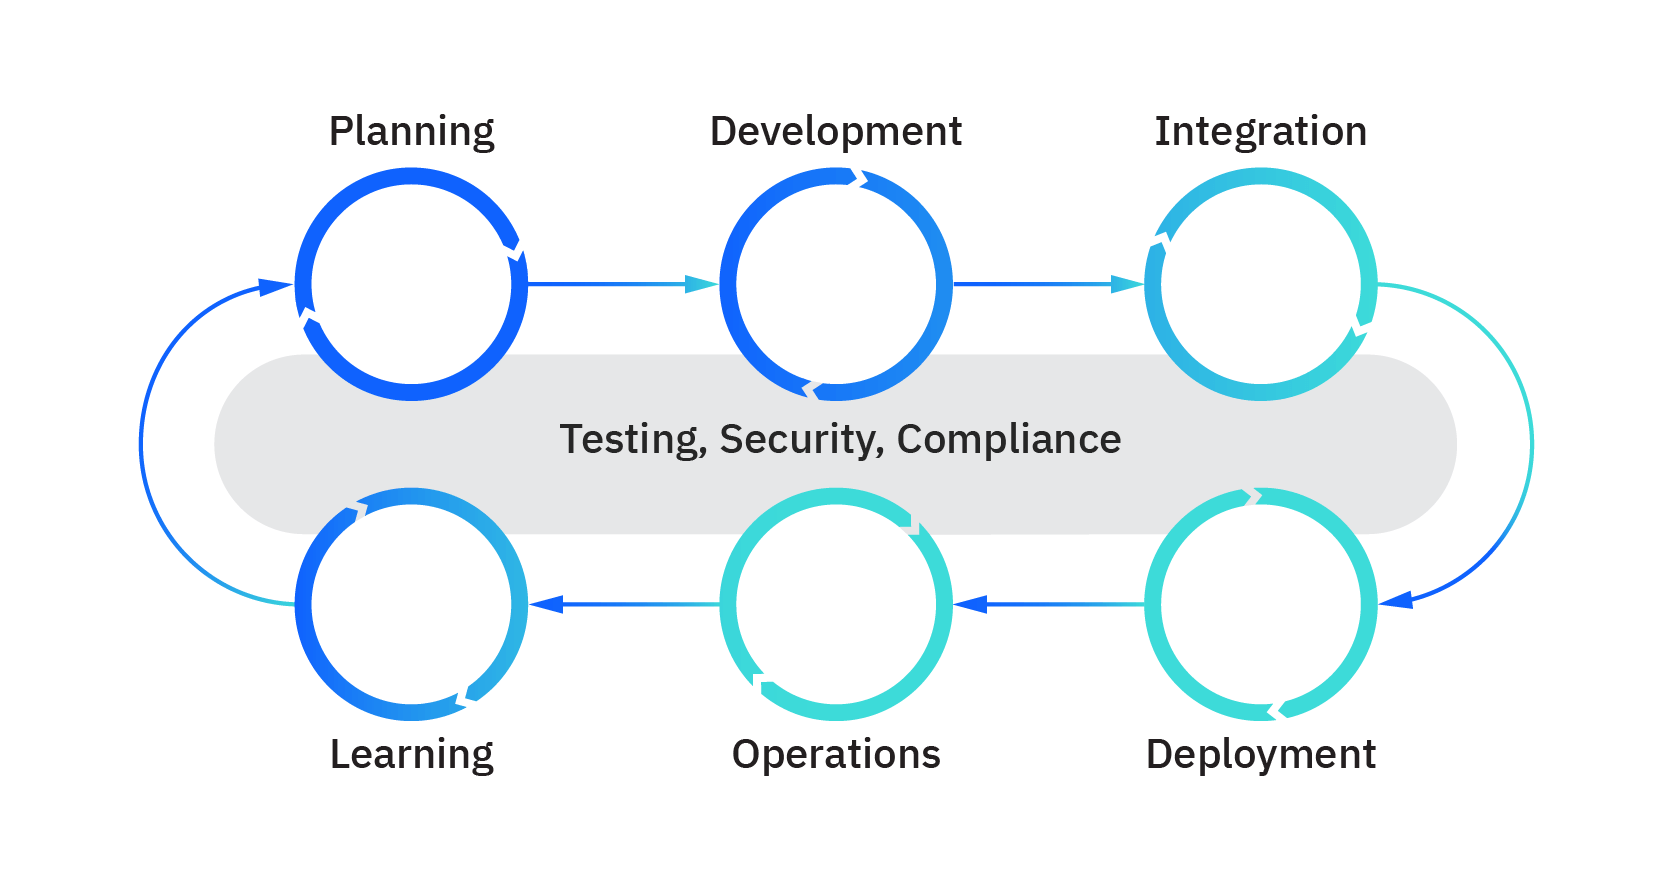
\includegraphics[width=\textwidth]{./assets/figures/ibm-devops-lifecycle.png}
        \caption[Cycle de vie de développement]{Cycle de vie de développement - IBM} \label{devops-lifecycle}
    \end{figure}
\end{center}

Aucun Devops ou pipeline n'avait été réalisé lors du précédent projet.\\
Nous avons donc que des propositions, sans solution existante (ce qui était le cas pour d'autres choix).\\
Avant de présenter chacun des pipeline DevOps proposé, il est nécessaire d'expliquer pourquoi chacun de ces derniers passent par Github, et plus précisément, les Github Actions.

\subsubsection{Pourquoi Github?}
Tout d'abord, il faut comprendre qu'il existe d'autres outil de "gestion" de \Gls{devops}, appelé
aussi services de \Gls{ci} / \Gls{devops}, en voici une liste non exhaustive:
\begin{multicols}{2}
    \begin{itemize}
        \item \href{https://www.jenkins.io/}{Jenkins},
        \item \href{https://www.jetbrains.com/teamcity/}{TeamCity},
        \item \href{https://www.guru99.com/top-20-continuous-integration-tools.html}{CircleCI},
        \item \href{https://www.travis-ci.com/}{Travis-CI},
        \item \href{https://about.gitlab.com/}{GitLab},
        \item \href{https://www.atlassian.com/software/bamboo}{Bamboo},
        \item \href{https://www.gocd.org/}{GoCD},
        \item \href{https://azure.microsoft.com/fr-fr/services/devops/}{Azure DevOps}.
    \end{itemize}
\end{multicols}

Tous ces outils, mise à part GitLab, doivent être installé en plus et configurer pour le projet.\\
Comme il s'agit d'un projet assez restreint et n'impliquant que peu de personnes, nous cherchons à rester dans une solution simple et donc "all in one".\\
Nous n'allons donc pas plonger dans les détails de chaque technologie citée plus haut.\\
Parmi les solutions "all in one", c'est-à-dire qui propose des services de \Gls{ci} / \Gls{devops} et permette le versioning de code, il reste uniquement GitLab et Github comme choix.\\
Ne souhaitant pas réaliser une profonde analyse sur ces 2 solutions, car les 2 étant souvent considérées comme équivalentes ou interchangeable, ma connaissance de la solution Github est un argument suffisant, selon moi, pour faire pencher la balance en sa faveur.
% Tous les outils CI / CD
%https://katalon.com/resources-center/blog/ci-cd-tools#
%https://www.lambdatest.com/blog/31-best-ci-cd-tools/
%https://www.guru99.com/top-20-continuous-integration-tools.html
%https://stackshare.io/stackups/github-actions-vs-gitlab-ci#pros

\subsubsection{Présentation des pipeline Devops possibles}

%\figi{devops-choix.drawio}{16cm}{Différents pipelines DevOps possibles}

Ce premier pipeline possible possède uniquement un intérêt si l'infrastructure de production tourne
à l'aide de conteneurs Docker. En effet, le but est de construire les images Docker contenant tout
ce qui est nécessaire (configurations, programmes, etc.) au niveau de la machine de développement,
puis d'envoyer ces dernières sur un repository d'image, en l'occurence, Dockerhub. Puis de
récupérer ces images sur la machine de production et de les lancer simplement.
%\figi{devops-dockerhub.drawio}{16cm}{DevOps via dockerhub}

Ce second pipeline, passerait par une plateforme appelée Heroku. Heroku permet de déployer son application sur l'un de leur serveur, puis le redéployer sur une machine de production finale.\\
Cette approche est très intéressante car l'étape intermédiaire permet de tester l'application sur une autre machine que celle de développement et ceci avant de livrer en production.
%\figi{devops-heroku.drawio}{16cm}{DevOps via heroku}
%https://devcenter.heroku.com/articles/getting-started-with-laravel

Finalement, le pipeline passant uniquement par Github, est la solution la plus simpliste en terme du nombre de technologies utilisées. Cette dernière repose sur le fait de simplement pousser le code sur Github et de le mettre à jour sur la machine de production via un script qui récupère les données sur le Github.
%\figi{devops-github.drawio}{16cm}{DevOps via github}

\subsubsection{Comparaison des pipeline Devops possibles}
Nous allons définir pour chacun des pipelines, les avantages et inconvénients de ces derniers.
Mais pour réaliser cette section, certains prototypes doivent être réalisés, ainsi que des recherches appronfidies sur la mise en oeuvre des différents pipeline.\\
En effet, n'étant pas expert dans le domaine, et n'ayant pas le temps de le devenir le temps de ce travail, l'un des critères / besoins importants et la facilité de mise en place du pipeline.

% pipeline docker
Commençons par le pipeline Docker \ref{devops-dockerhub}.
\begin{table}[h]
    \begin{center}
        \caption{pipeline Docker / Dockerhub \label{devops-dockerhub}}
        \begin{tabularx}{1.0\textwidth} {X|X}
            Avantages & Inconvénients \\ \hline
                      &               \\
                      &               \\
                      &               \\
                      &               \\
                      &               \\
        \end{tabularx}
    \end{center}
\end{table}

Continuons avec le pipeline Heroku \ref{devops-heroku}.
\begin{table}[h]
    \begin{center}
        \caption{pipeline Heroku \label{devops-heroku}}
        \begin{tabularx}{1.0\textwidth} {X|X}
            Avantages & Inconvénients \\ \hline
                      &               \\
                      &               \\
                      &               \\
                      &               \\
                      &               \\
        \end{tabularx}
    \end{center}
\end{table}

Finissons avec le pipeline Github \ref{devops-github}.
\begin{table}[h]
    \begin{center}
        \caption{pipeline Github \label{devops-github}}
        \begin{tabularx}{1.0\textwidth} {X|X}
            Avantages & Inconvénients \\ \hline
                      &               \\
                      &               \\
                      &               \\
                      &               \\
                      &               \\
        \end{tabularx}
    \end{center}
\end{table}

% TODO reciter besoins et dire solution qui se rapproche le plus

%\clearpage
%\subsection{Système de gestion de base de données}
% postgre vs mysql
%https://www.geeksforgeeks.org/difference-between-mysql-and-postgresql/
%https://www.simplilearn.com/tutorials/sql-tutorial/postgresql-vs-mysql
%https://www.ibm.com/cloud/blog/postgresql-vs-mysql-whats-the-difference
%https://stackshare.io/stackups/mysql-vs-postgresql

% upgrade to laravel 9
%https://laravel.com/docs/9.x/upgrade
%https://github.com/laravel/vonage-notification-channel/blob/3.x/UPGRADE.md

% \begin{center}
%     \begin{figure}
%         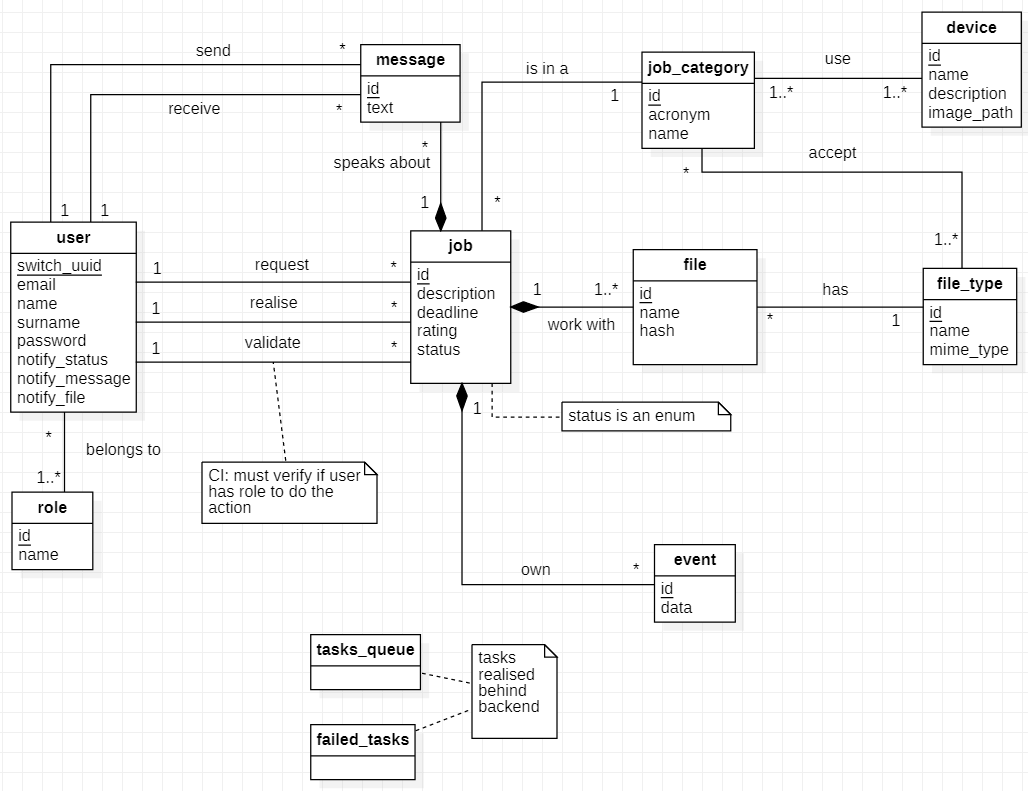
\includegraphics[width=\textwidth]{./assets/figures/ea.png}
%         \caption[Stack de technologies]{Stack de technologies utilisées via \href{https://stackshare.io/alecberney/bachelors-thesis \label{stack-tb}}}
%     \end{figure}
% \end{center}

\chapter{Github et code}
Avant de commencer à parler de conception et de réalisation, il est nécessaire de parler de la façon dont les projets sont stockés et gérer.

\section{Association GitHub}
La première chose réalisée est d'avoir créer une association Github au nom du \href{https://github.com/heig-fablab}{heig-fablab}. C'est un point important car cela permet de regrouper plusieurs \Gls{repository} sous le même "groupe de travail", la même association.

\section{Repositories}
Dans cette association, trois \Gls{repository} ont été créés, les voici:
\begin{itemize}
    \item \href{https://github.com/heig-fablab/fablab-manager}{fablab-manager} étant le \Gls{repository} principal contenant le \Gls{backend} et le \Gls{frontend} compilé et minimisé pour la production,
    \item \href{https://github.com/heig-fablab/fablab-manager-frontend}{fablab-manager-frontend} étant le \Gls{repository} contenant le code du {frontend},
    \item \href{https://github.com/heig-fablab/heig-keycloak-auth-token}{heig-keycloak-auth-token} étant un \Gls{repository} permettant de faciliter le développement du \Gls{backend};
\end{itemize}

\section{README}
Chaque \Gls{repository} contient un fichier "README.md" indiquant toutes les instructions à suivre afin d'installer l'environement de développement lié au \Gls{repository} ainsi que quelques informations supplémentaires utiles tel que les versions des outils utilisés pour le développement.

Les \Gls{repository} sont rédigés en anglais afin de pouvoir transmettre le plus aisément possible le projet.

\section{Wiki}
Le \Gls{repository} fablab-manager étant le principal, ce dernier possède également un wiki avec énormément d'informations concernant la conception et la réalisation du projet. On peut notamment retrouver une majorité des informations disponibles dans ce rapport.

\section{Issues Github}
Ce \Gls{repository} liste également toutes les tâches réalisées et à réaliser du projet. Ces tâches sont répertoriées sous forme d'"issue" \Gls{github}. Ces dernières indique grâce à des labels s'il s'agit d'un bug, de la documentation, un ajout, etc. et si elles appartiennent au projet \Gls {frontend} ou \Gls{backend} ou les deux.

\section{Kanban}
Les "issues" abordées, il est maintenant nécessaire de parler du "kanban" mis en place. Le "kanban" est un tableau contenant toutes les "issues" et les rangeants dans des catégories en fonction de l'avancement de la tâche / "issue". \\
Le "kanban" que j'ai créé contient 5 colonnes:
\begin{itemize}
    \item backlog représantant toutes les tâches / "issues" à mettre en place sur le projet à terme,
    \item todo (actual sprint) représantant toutes les tâches / "issues" à réaliser pendant le sprint actuel,
    \item in-progress indiquant toutes les tâches / "issues" en cours de réalisation,
    \item done but can be modified indiquant les tâches / "issues" terminée mais pouvant être re-modifiée.
    \item done représentant les tâches / "issues" terminées et fermées.
\end{itemize}

\section{Milestones}
Pour m'organiser et travailler d'une manière agile, j'ai créé des milestones représantant les sprints que j'allais réaliser durant le projet. Une milestone spécial s'y est glisser, elles est nommée "nice to have" est représente toutes les tâches non inclues dans le cahier des charges ou non prioritaires / nécessaires mais étant intéressantes à ajouter au projet.

\section{Git flow / Workflow}
Même si j'étais seul lors de ce projet, j'ai prévu qu'il soit potentiellement maintenu par plusieurs personnes à la fois, j'ai donc établi un Git flow ou Workflow afin de faciliter la collaboration. Ce dernier suit un standard bien établi et est consultable à la figure \ref{git-flow}.

\begin{center}
    \begin{figure}
        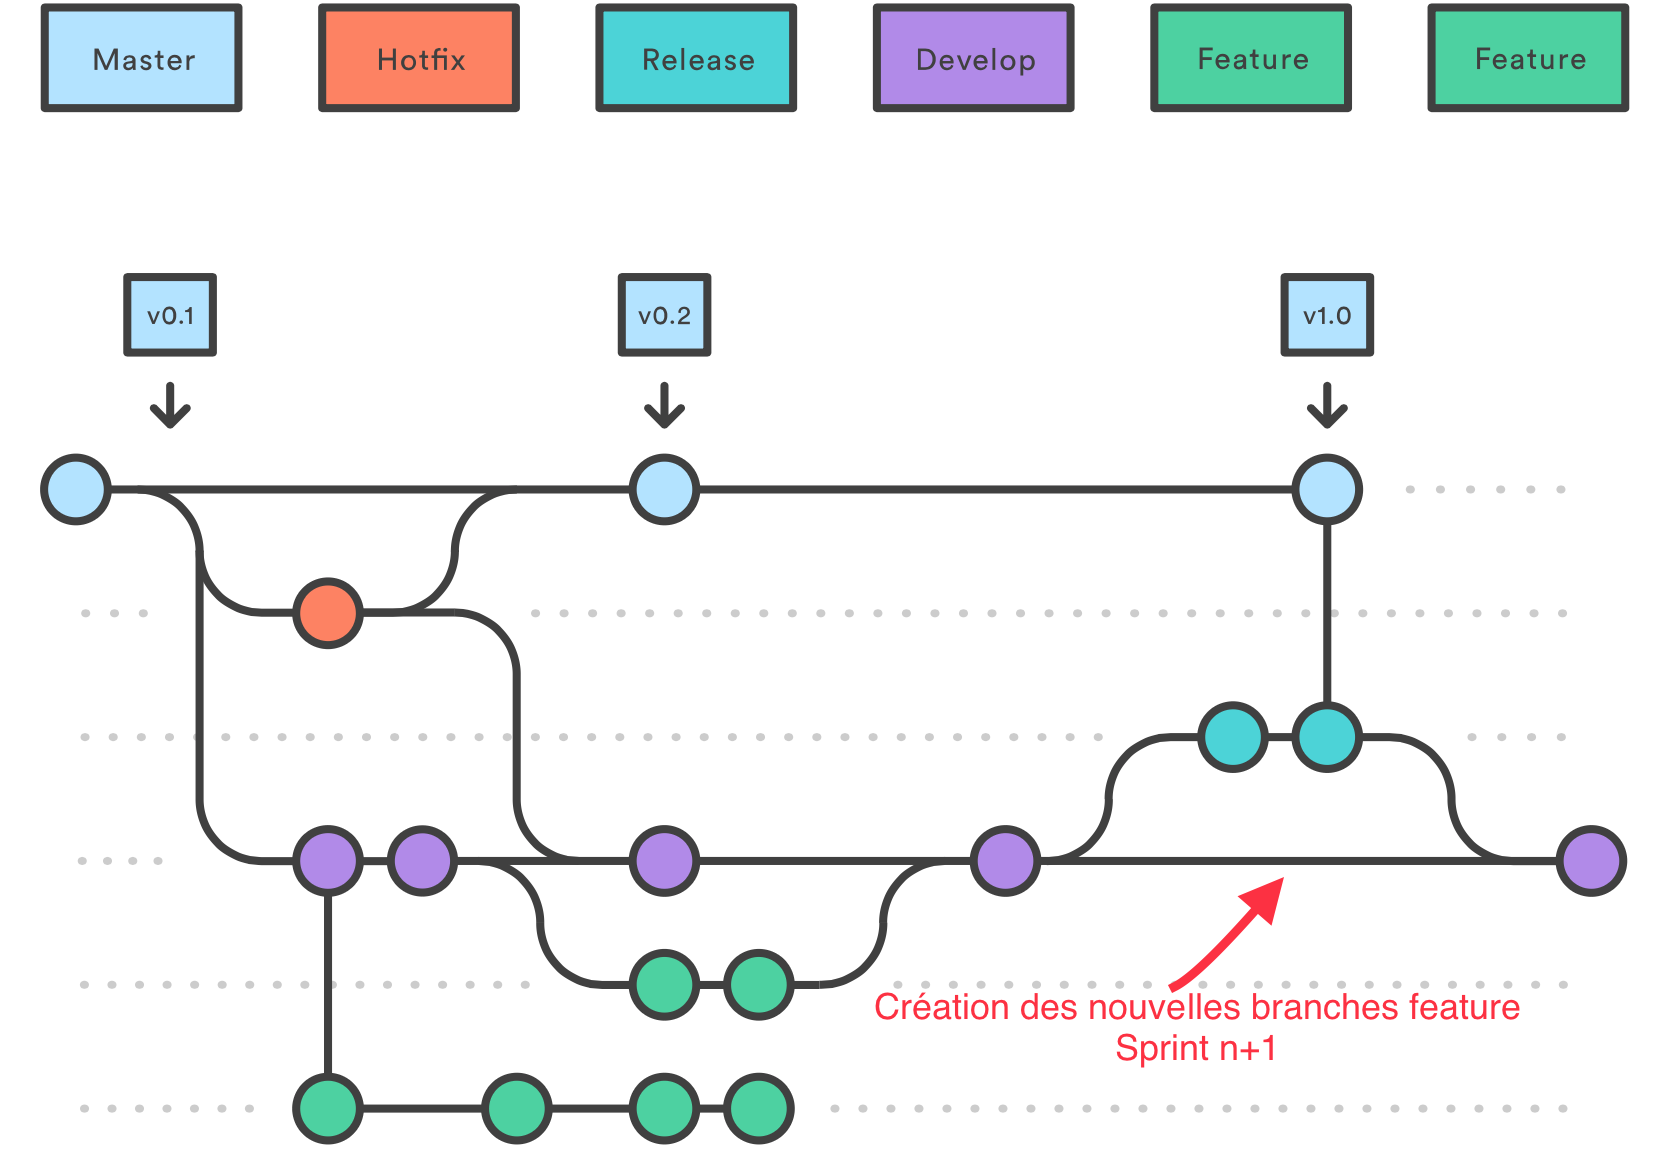
\includegraphics[width=\textwidth]{./assets/figures/git-flow.png}
        \caption{Git flow \href{https://www.atlassian.com/fr/git/tutorials/comparing-workflows/gitflow-workflow} \label{git-flow}}
    \end{figure}
\end{center}

% cliffhanger
Maintenant les outils de travail ont été définis, nous pouvons passer à la conception et la réalisation de la base de données, racine de tout projet avec stockage de données.

\chapter{Conception et Réalisation de la BD}

Dans toutes les desciptions suivantes, les tirets du bas seront remplacé par des "-" à cause d'un problème de LaTex.

\section{Modèle EA}
Le modèle Entité-Associations est la première étape lors de la conception d'une base de données. Il se rapproche également d'un diagramme de classe classique utiliser pour la POO (programmation orienté objet).\\
Nous allons décrire chacune des entités et ses relations.\\
Mais avant ça, voici quelques informations sur le schéma, une sorte de légende:\\
Un rectangle représente une entité et possède son nom dans sa partie supérieur.\\
Les valeurs textuelles en dessous sont les champs de l'entité. Le champ souligné représente la clé primaire de l'entité, cette dernière doit être unique.\\
Les traits tiré entre deux entités sont des associations et peuvent se lire dans les deux sens. Les verbes écrits au dessus des traits servent à donner un sens à l'association.\\
Les symboles et numéros à chaque extrémités des entités indiquent respectivement:
\begin{itemize}
    \item 0 : zéro / aucun,
    \item 1 : un,
    \item 1..* : un ou plusieurs,
    \item * : zéro ou plusieurs.
\end{itemize}

Par exemple, on peut lire l'association "user" - "message", comme ceci:\\
Un utilisateur peut envoyer zéro ou plusieurs messages.\\
Un message peut être envoyé que par un utilisateur.

Finalement, quelques commentaires peuvent être ajouté avec des rectangles pliés en haut à droite et relié avec des traits pointillés.

\begin{center}
    \begin{figure}
        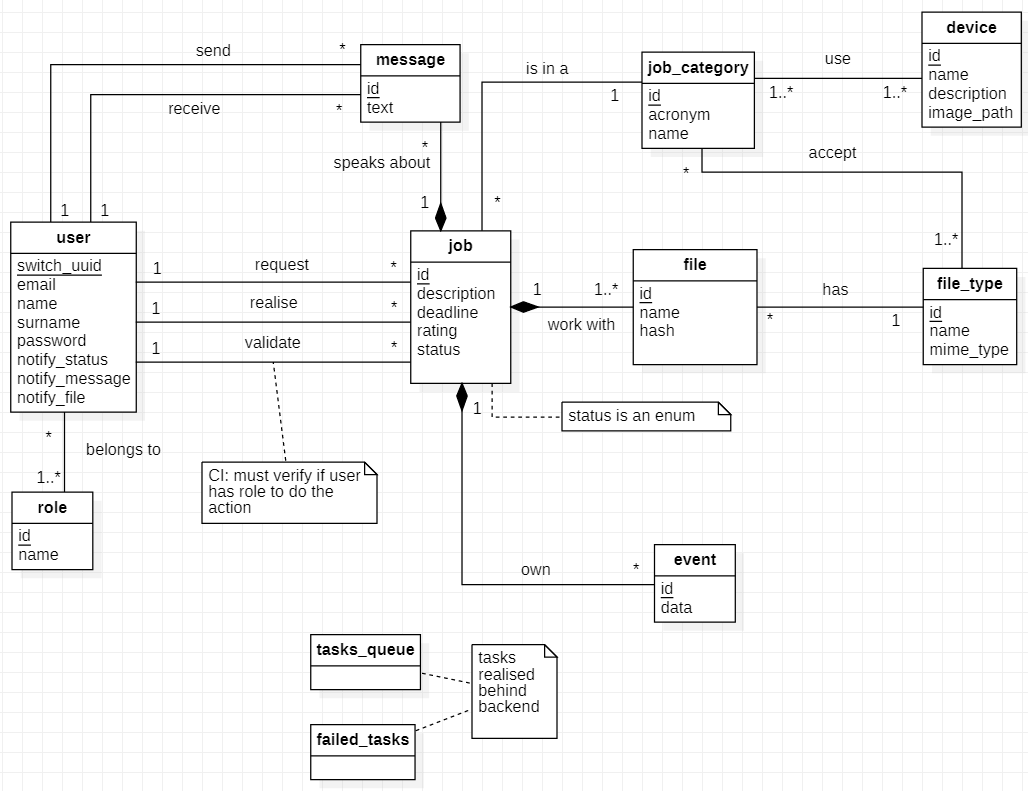
\includegraphics[width=\textwidth]{./assets/figures/ea.png}
        \caption{Modèle EA \label{ea}}
    \end{figure}
\end{center}

\subsection{Entité user}
L'entité "user" représente un utilisateur de l'application, que ce soit un élève, un professeur ou un technicien.\\
Il possède des informations classiques le concernant, ainsi que le champ "switch-uuid" représentant l'identifiant unique fourni par le service Switch edu-id qui sera utilisé.\\
Les champs contenant le mot "notify" servent à stocker les préférences de l'utilisateur concernant les notifications de l'application.

On voit au niveau des relations, que l'utilisateur peut envoyer et recevoir des messages.\\
Il peut posséder également plusieurs rôles mais doit en posséder au moins un, celui par défaut qui est le rôle "client".\\
L'utilisateur peut de toute façon faire une demande de travail (job). Cependant, seul les utilisateurs possédant le rôle "validator", en général, les professeurs pourront valider le travail.\\
Le travail validé, un "worker", en général un technicien, pourra réaliser le travail demander et en indiquer le suivi.

\subsection{Entité job}
L'entité "job" représente un travail demandé par un utilisateur de l'application.\\
Il possède un id (identifiant unique), une description du travail à réaliser, une date butoir (deadline), une évaluation que l'utilisateur / client peut attribuer au travail terminé et un status d'avancement du travail mis à jour par le travailleur.\\
Le status d'avancement d'un travail sera défini par un enum (liste exhaustive de valeurs), la voici:
\begin{itemize}
    \item new,
    \item validated,
    \item assigned,
    \item ongoing,
    \item on-hold,
    \item completed.
\end{itemize}

On voit au niveau des relations, que le travail peut posséder des messages qui lui sont liés.\\
Il posséde également une catégorie de travail définissant ensuite quelles machines peuvent être utilisées pour le réaliser.\\
Le travail possédera également un utilisateur client, un validateur et un travailleur.\\
Il doit également contenir un ou plusieurs fichiers nécessaires pour réaliser le travail demandé.\\
Finalement, certains événements peuvent être lié au travail. On parle ici d'événement permettant de préfevenir l'utilisateur via des notifications ou email.

\subsection{Entité role}
L'entité "role" représente simplement un rôle que peut avoir un utilisateur au sein de l'application. Cette entité est nécessaire car un utilisateur peut posséder plusieurs rôles et ils doivent tous être défini la même chose.\\
Seul un id (identifiant unique) et un nom du rôle est nécessaire.\\
Voici la liste des rôles définis:
\begin{itemize}
    \item admin,
    \item client,
    \item worker,
    \item validator.
\end{itemize}

\subsection{Entité message}
L'entité "message" représente un message envoyé entre deux utilisateurs au sujet d'un travail demandé.\\
Il possède uniquement un id (identifiant unique) et un texte.\\
Il est associé à deux utilisateurs, un représentant celui qui a envoyé le message et l'autre celui qu'il l'a reçu. Le message est également associé au travail dont il est le sujet.\\
Une aggrégation a été modélisé pour cette dernière association car on souhaite supprimé tous les messages liés à un travail, si ce dernier est supprimé.

\subsection{Entité job-category}
L'entité "job-category" représente une catégorie de travail pouvant être effecutée au Fablab, pare exemple, une impression 3D ou une découpe laser.\\
La catégorie possède un id (identifiant unique), un acronyme et un nom.\\
Elle est associé à un travail car ce dernier est obligé d'avoir une catégorie.\\
Elle possède également une ou plusieurs machines (device) sur lesquels peuvent être réaliser les travaux.\\
Comme elle possède des machines, une liste de type de fichiers acceptés est nécessaire et est défini par l'association "job-category" - "file-type". Cela permettra de facilement vérifier si un fichier donné pour un travail peut être accepté pour la catégorie de ce dernier.

\subsection{Entité device}
L'entité "device" représente une machine / un outil utilisé pour réaliser un travail du Fablab.\\
La machine possède un id (identifiant unique), un nom, une description plus précise et un chemin de fichier où est stocké son image (cette partie pourrait changer).\\
Comme expliqué précédement dans la catégorie, elle possède une ou plusieurs catégories sur lesquels elle peut être utilisée.\\

\subsection{Entité file-type}
L'entité "file-type" représente un type de fichier que peut accepter une catégorie de travail du fablab.\\
Le type de fichier possède un id (identifiant unique), un nom et un \href{https://developer.mozilla.org/fr/docs/Web/HTTP/Basics_of_HTTP/MIME_Types}{mime-type} étant utiliser pour valider les fichiers télécharger.\\
Comme expliqué précédement dans la catégorie, un type de fichier possède une ou plusieurs catégories qui sont acceptées.\\
Le type de fichier peut également être associé à plusieurs fichiers.

\subsection{Entité file}
L'entité "file" représente un fichier fourni pour réaliser un travail du Fablab.\\
Le fichier possède un id (identifiant unique), un nom et un hash de son contenu.\\
Il est associé à un type de fichier (file-type), ce qui est utile pour faire le lien avec la catégorie du travail.\\
Il possède évidemment un travail pour indiquer pour auquel il appartient.\\
Une aggrégation a été modélisée pour cette dernière association car on souhaite supprimé tous les fichiers liés à un travail, si ce dernier est supprimé.

\subsection{Entité event}
L'entité "event" représente un événement concernant un travail du fablab. Par exemple, un événement est généré si le status d'un travail a été modifié ou si un fichier a été ajouté. \\
L'événement possède un id (identifiant unique) et des données (data).\\
Il est associé à un travail comme expliqué plus précédement.\\
Une aggrégation a été modélisée pour cette dernière association car on souhaite supprimé tous les événements liés à un travail, si ce dernier est supprimé.

\subsection{Entité tasks-queue et failed-tasks}
Ces entités ont été modélisées pour effectuer les tâches en arrière plan du backend, comme l'envoi d'email retardé. Elle ne sont pas encore très développée par manque de connaissances de leur fonctionnement.

\section{MLD}
Le modèle logique des données n'est rien d'autre qu'une évolution du modèle EA.\\
Les entités deviennent des tables et les associations des relations, ce qui est presque la même chose.\\
Les tables ont pris un nom au pluriel pour respecter la philosophie de Laravel et de son \Gls{orm} Eloquent.\\
Les champs obtiennent des types représentant la façon dont ils seront stockés.\\
Les clés étrangère issues des association s'ajoutent aux tables.\\
Les associations N à N du modèle EA voient naître une table intermédiaire. Voici celles qui ont été créées:
\begin{itemize}
    \item device-job-category,
    \item file-type-job-category,
    \item role-user.
\end{itemize}

\begin{center}
    \begin{figure}
        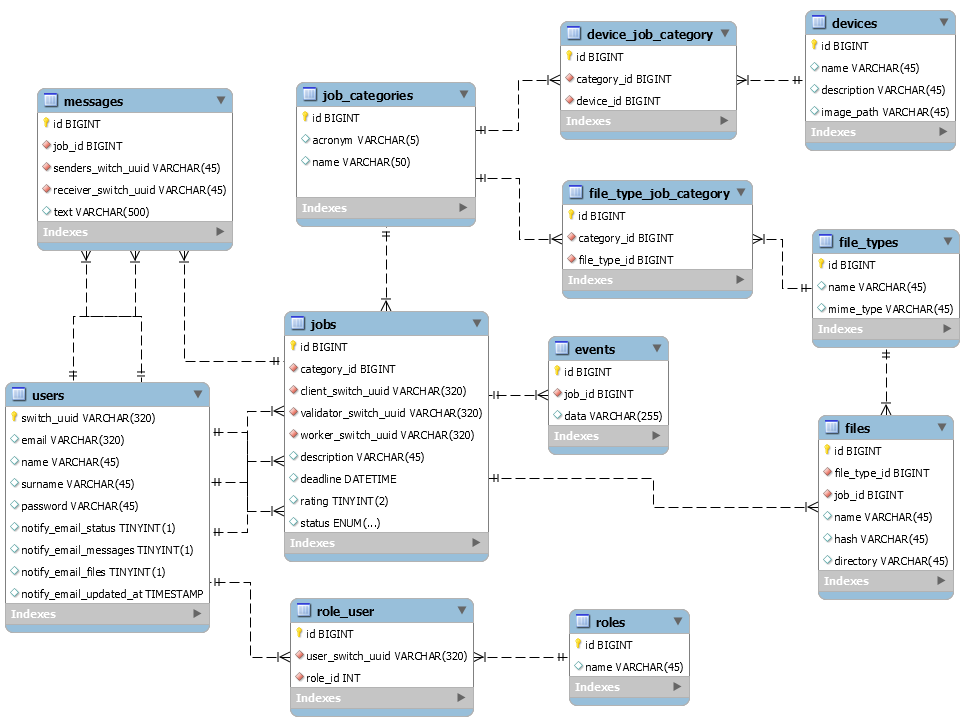
\includegraphics[width=\textwidth]{./assets/figures/mld.png}
        \caption{Modèle Logique des données \label{mld}}
    \end{figure}
\end{center}

Sur le schéma, quelques nouveaux symboles apparaîssent, voici une légende:
\begin{itemize}
    \item Clé jaune : clé primaire de la table,
    \item Losange bleu : la colonne ne peut pas valoir null,
    \item Losange vide : la colonne peut valoir null,
    \item Losange rouge : la colonne possède une clé étrangère.
\end{itemize}

Une clé étrangère étant le champ représantant une autre table issue d'une relation existante. La clé primaire représente la table en elle-même, elle est son identifiant.

\subsection{Champs spéciaux}
Quelques champs obtiennent des valeurs précises et méritent une explication.\\
Les champs switch-uuid et email, de la table "users" possèdent 320 charactères car ils sont tous
deux des emails ou des dérivés et une email peut contenir au maximum 320 charactères \cite{email-length}.

Le champ status de la table "job" est une enum comme expliqué précédement dans le modèle EA.

\subsection{Remarques}
% TODO une fois défini
Tous les autres champs n'ont pas encore fait l'objet de recherches ou de spécifications et ont donc souvent une valeur de 45 ou 50 charactères. Cela cera réalisé prochainement.

Les entités concernant les tâches en arrière plan n'apparaîssent pas car elle ne sont pas encore assez connue.

%Certaines colonnes sont communes à plusieurs des tables. C'est le cas de 'created_at',
%qui indique l'heure de création de la ligne, et 'updated_at', qui indique l’heure à
%laquelle la ligne à été modifiée pour la dernière fois.


\section{Migrations Laravel}

Les migrations du backend réalisées avec Laravel et l'ORM Eloquent se rapprochent le plus possibles du MLD présenté précédement.

\subsection{Types de champs}
Voici une liste des types possibles et utilisées:
\begin{itemize}
    \item id: un entier positif incrémentable, unique, indiqué comme clé primaire et référencé via un index,
    \item string: une chaîne de caractères,
    \item longText: un grand texte,
    \item enum: une liste exhaustive de valeurs possibles,
    \item tinyInteger: un petit entier,
    \item date: une date.
\end{itemize}

La liste plus complète peut être consultée dans la doc \href{https://laravel.com/docs/9.x/migrations#available-column-types}{Laravel}.

\begin{listing}[h]
    \inputminted{php}{assets/code/12_create_file_types_table.php}
    \caption{Migration de la table "file-types" \label{migrations-file-types}}
\end{listing}

\subsection{Champs possiblement "null"}
La possibilité de laisser une valeur nulle sur un champ n'apparaît pas sur le MLD, mais est bien présente au niveau des migrations et modèles de Laravel.\\
Tous ces champs possèdent l'indiquation: "->nullable()".\\
Seul certains champs peuvent être "null" dans notre base de données et ceux-ci interviennent surtout dans la table "jobs".\\
Les champs qui peuvent être "null" sont des champs dont la valeur n'est pas obligatoirement présente à la création mais peut-être ajoutée plus tard. Il s'agit par exemple de la note donnée au travail "rating" ou encore le technicien devant effectuer ce dernier qui peut être assigné après coup.

\subsection{Champs uniques}
Il est possible d'indiquer qu'un champ doit posséder une valeur unique avec l'option: "->unique()".\\
Cette possibilité est par exemple utilisée par le champ email.

\subsection{Champs timestamps}
Les champs de type "->timestamps()" sont un raccourci utilisé par Laravel pour créer deux champs indiquant la date de création de la donnée et la date de modification. Ces champs sont gérés automatiquement par Laravel, ce qui est bien pratique.

\subsection{Indexes}
Il est possible de créer des indexes sur certains champs afin d'améliorer les performances de la base de données lors de certaines requêtes. Ces indexes peuvent être créer grâce à l'instruction "index('table-champ')".\\
Ces derniers sont toujours créer sur les clés primaires et doivent être créer sur les clés étrangères. D'autres champs régulièrement utilisés par des requêtes peuvent faire l'objet d'indexes.

\subsection{Clés étrangères}
Les clés étrangères peuvent être gérées de deux façon différentes.\\
Soit on ajoute un champ "foreignId('table-id')" suivi d'un "->constrained('table')" qui permet de faire le lien directe entre la clé primaire et la clé étrangère tout en générant un index. Mais ceci est possible uniquement si l'on utilise une clé primaire de type "id()".

Dans le deuxième cas, lorsque l'on possède une clé primaire basée sur un autre type de champ, il faut tout d'abord créer un champ à la main avec la valeur voulue.\\
Puis faire le lien entre la clé primaire et étrangère à la main en utilisant d'abord "->foreign('table-champ')", puis en référançant avec "->references('champ')->on('table')".\\
Puis, finalement, créer un index avec "index('table-champ')" sur le champ de la clé étrangère.

\subsection{Options de suppression}
Des options de suppression sont proposées par \Gls{eloquent} afin de ne pas supprimer définitivement les données de la base de données, mais de simplement les désactiver afin quelles n'apparaîssent plus dans les requêtes.\\
Ceci est possible en ajoutant l'option "->softDeletes()" à la table.\\
Laravel s'occupera ensuite de gérer les cas de suppression lui-même.

\chapter{Conception et Réalisation du Backend / de l'API}

\section{Architectures de code}

Ne connaissant pas le framework Laravel à l'origine, mais plutôt celui de Java Spring, j'ai effectué
un schéma de l'architecture de code de ce dernier afin de le comparer avec celui de Laravel et
pouvoir mieux le comprendre. Sur la figure \ref{architecture-code-spring.drawio}, on voit clairement
l'architecture classique allant de la vue passant par les controllers, puis les services contenant
la logique métier et les repository utilisant les DAO pour commumiquer avec la base de données. \\
Des DTO peuvent également être ajoutées entre la vue et les controllers.

%\figi{architecture-code-spring.drawio}{16cm}{Architecture de code du framework Spring "classique"}

J'ai ensuite essayé de comprendre l'architecture de code Laravel et la représenté à l'aide de la
figure \ref{architecture-code-laravel.drawio}.

%\figi{architecture-code-laravel.drawio}{16cm}{Architecture de code du framework Laravel "classique"}

Je ne comprenais pas où la logique métier (business logic) devait être codée et je pensais donc
ajouter des services comme l'architecture de code Spring le fait si bien. Cela donnait une
architecture correspondant à la figure \ref{architecture-code-laravel-proposee.drawio}.

%\figi{architecture-code-laravel-proposee.drawio}{16cm}{Architecture de code Laravel proposée}

Finalement après m'être plus plongé dans le code et la documentation, je me suis rendu compte que
Laravel proposait beaucoup plus de classe ou d'outil de code que ce que j'avais pu comprendre en
premier temps. J'ai donc mis à jour l'architecture de code finale et cette dernière suivra le schéma
de la figure \ref{architecture-code-finale.drawio}.

Nous allons maintenant discuté de quelques pattern de code utilisé et fourni par Laravel.\\
Tout d'abord, on peut observer que les middleware utiliseront l'AuthServiceProvider qui
implémentera des Gates. Ces Gates utiliseront des Policy qui permettront de définir la logique afin
de valider si l'utilisateur possédera ou non le droit d'accès à l'action sur la route utilisée de
l'API utilisée. Par exemple, il sera vérifier que seul un technicien ou un validateur puisse mettre
à jour le statut de la demande.

Ensuite, on observe que les Controllers vont recevoir des ModelRequests représentant des requêtes
contenant les valeurs nécessaires. Les valeurs à l'intérieur des requêtes seront exhaustivement
définies et syntaxiquement validées. Cela permettra de travailler avec des valeurs sûrs au niveau
des Controllers et des Models. Par exemple, il sera possible de valider qu'un email donné soit un
email syntaxiquement correct.

Les Controllers travailleront avec des Resources (ressources) afin de retourner uniquement les
valeurs voulues. Ces Resources définissent exactement ce qui doit être renvoyer, comme données, à
l'utilisateur. Il sera par exemple possible de définir que le mot de passe de l'utilisateur ne soit
pas retourné à ce dernier. Ces Resources utilisent également des ResourcesCollection permettant de
définir des collections de ressources lorsqu'une route doit fournir plus qu'un seul élément.

%\figi{architecture-code-finale.drawio}{16cm}{Architecture de code Laravel finale}

% cliffhanger
Avant de passer aux détails d'implémentation de cette architecture de code, il est nécessaire de définir les routes que l'\Gls{api} fournit.

\section{Routes}
Les routes définies par l'\Gls{api} sont organisée par modèle / ressource et sont ensuite trier par action possible. \\
Voici la liste des ressources sur lesquels certaines actions peuvent être exécutées:
\begin{itemize}
    \item files,
    \item file types,
    \item job categories,
    \item jobs,
    \item messages,
    \item users;
\end{itemize}

Le détail de ces routes est consultable sur la figure \ref{routes-api}.
\begin{listing}[h]
    \inputminted{php}{assets/code/api.php}
    \caption{Routes de l'API \label{routes-api}}
\end{listing}

On remarque aisément que la route principale est la route "jobs" et que toutes les autres routes sont également liées à cette dernière. On peut également remarquer que la route "file types" est uniquement réservé aux administrateurs.

\subsection{REST}
Les routes fournies essaient au maximum de suivre le principe \Gls{rest}. \\
Toutes les routes indiquant la méthode "GET" servent uniquement à récupérer des informations.
Les routes avec la méthode "POST" à créer une nouvelle donnée / entrée. \\
Les routes avec la méthode "PUT" à mettre à jour les données d'une entrée. \\
Les routes avec la méthode "PATCH" à mettre à jour seulement certaines données spécifiques d'une entrée. \\
Les routes avec la méthode "DELETE" à supprimer une entrée.

On remarque également qu'il a été choisi d'insérer l'id de l'entrée mise à jour (méthode "PUT") au niveau des données "body" de la requête et non dans la "query string". Le but étant de regrouper toutes les informnations / données à vérifier au même endroit. \\
La majorité des routes avec la méthode "PATCH" suivent le même principe. Une exception a été faite pour la route "PATCH /api/jobs/{id}/notifications/user/{username}" car aucune donnée ne doit être transmise ne plus du job et de l'utilisateur concerné. Il était donc plus simple et lisible de passer les informations dans la query string.

% cliffhanger
Maintenant les routes définies et connues, il est nécessaire de parler de ce qu'il faut fournir et ce qui est nécessaire de fournir pour les utiliser. Nous allons donc voir comment l'authentification pour accéder à l'API a été mise en place.

\section{Authentification}

\subsection{Choix du système d'authentification}
Pour l'authentification, nous avions 2 possibilités, utiliser le système de l'école ou utiliser \href{https://www.switch.ch/edu-id/}{Switch edu-ID}. Switch edu-ID utilisant \href{https://www.switch.ch/aai/about/shibboleth/}{Shibboleth} et le système de l'école \href{https://www.keycloak.org/}{Keycloak}.

Shibboleth a comme désavantage d'être un outil supplémentaire à ajouter à la machine de production, de ne pas être simple à mettre en place et d'être difficilement testable et utilisable en phase de développement. \\
Il possède comme avantage de toucher un plus grand nombre d'utilisateur et d'avoir déjà été mis en place lors de l'ancien travail de Bachelor.

Keycloak étant basé sur \href{https://openid.net/connect/}{OpenID}, il a comme avantage de fournir un \Gls{jwt} et d'ensuite pourvoir l'utiliser afin de vérifier l'identité de l'utilisateur grâce à une signature également fournie par Keycloak. Un formulaire de connexion / d'authentification est également fourni avec l'outil. Un autre avantage et que l'école possède une totale maîtrise de l'outil et cela facilite grandement la mise en place et collaboration. \\
L'outil a comme désavantage de restreindre l'authentification aux membres de l'école \Gls{heig-vd}.

%todo expliquer différences entre openID, SAML et OAuth2
%https://www.parallels.com/blogs/ras/oauth-vs-saml-vs-openid/#:~:text=While%20the%20use%20cases%20for,than%20SAML%20and%20OpenID%20Connect.

% cliffhanger
Le système d'authentification Keycloak a finalement été choisi, me paraîssant le plus adapté. \\
Il est maintenant nécessaire de définir son fonctionnement plus en détail.

\subsection{Fonctionnement de Keycloak}
En résumé, l'outil Keycloak permet à l'école d'utiliser les utilisateurs de leur domaine et donc de leur \Gls{ad} afin d'authentifier une personne. Tout ceci en fournissant un formulaire de connexion et renvoyant un \Gls{jwt} une fois l'authentification réussie.

En consultant la figure \ref{keycloak-flow} et l'image \ref{}, On comprend bien que l'utilisateur arrivant sur le site, commence par s'authentifier à l'aide de ses informations d'identification, puis récupère un \Gls{jwt} agissant comme certificat / clé d'accès afin d'effectuer des requêtes au \Gls{backend}. \\
Ce token / jeton est ensuite ajouter dans l'entête de chaque requête vers le \Gls{backend}. \\
Lorsque le \Gls{backend}, reçoit une requête, il vérifie le jeton donné grâce à une signature fournie par le domaine Keycloak de la \Gls{heig-vd} et détermine si ce dernier et valable ou non.

%\figi{keycloak-flow.drawio}{16cm}{Flow de Keycloak}

\begin{center}
    \begin{figure}
        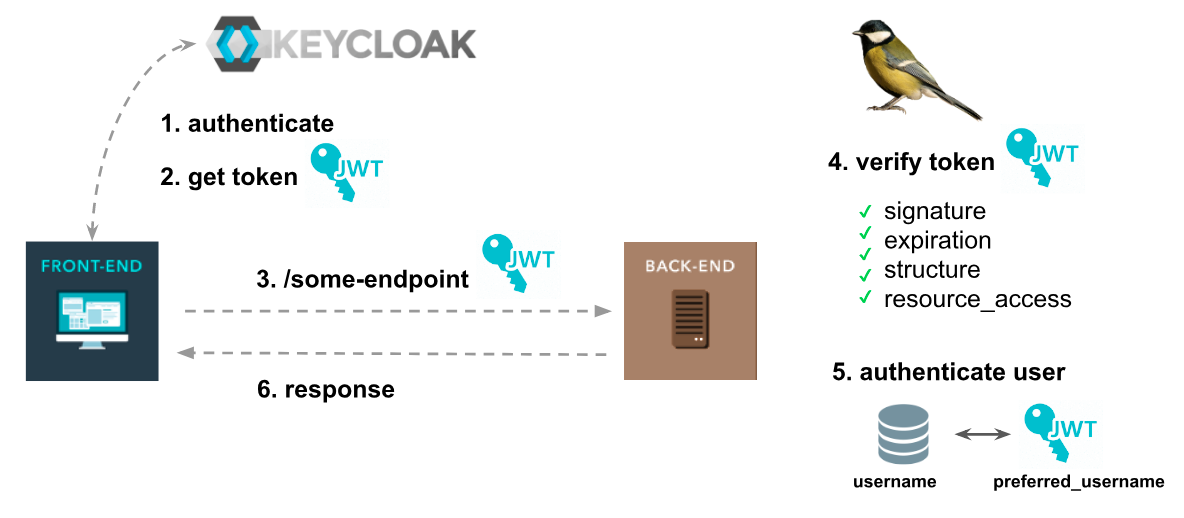
\includegraphics[width=\textwidth]{./assets/figures/keycloak-flow.png}
        \caption{Flow de Keycloak tiré de \href{https://github.com/robsontenorio/laravel-keycloak-guard} \label{keycloak-flow-lib}}
    \end{figure}
\end{center}


Le fonctionnement de Keycloak expliqué, il est nécessaire d'expliquer la façon dont il a été implémenté au niveau de Backend.

\subsection{Implémentation de Keycloak côté Backend}
Tout d'abord, on peut remarque sur la figure \ref{routes-api}, que l'authentification est utilisée dans le middleware "auth:api". Ce dernier étant appliqué à toutes les routes de l'\Gls{api}.

Pour ensuite implémenter la logique utilisée par ce middleware, je me suis inspiré d'un packet Laravel existant, \href{https://github.com/robsontenorio/laravel-keycloak-guard}{laravel-keycloak-guard}. Je n'ai pas pu l'utiliser direcement, car il n'était pas totalement adapté à nos besoins.

Pour intégrer mon adaptation de package au projet, j'ai d'abord créer un "KeycloakServiceProvider" comme on peut le voir à la figure \ref{keycloak-service-provider}. \\
Dans ce dernier on voit que l'on défini la "KeycloakGuard" pour l'authentification.

\begin{listing}[h]
    \inputminted{php}{assets/code/KeycloakServiceProvider.php}
    \caption{KeycloakServiceProvider \label{keycloak-service-provider}}
\end{listing}

Ensuite, on implémente la "KeycloakGuard" dans un fichier et une classe à part (disponible en annexe \ref{keycloak-guard}). Il est également nécessaire de définir quelques Exception liées à cette implémentation. \\
Tous ces fichiers sont disponibles dans le dossier /app/Providers/Keycloak.

De plus, il est nécessaire d'ajouter un fichier de config afin de supporter certains paramètres à fournir dans le ".env" tel que la clé publique permettant de vérifier les tokens. Ce fichier de config doit être créer dans le dossier "config" et se nommer "keycloak.php". Ce dernier est défini comme sous la figure \ref{keycloak.php}.

\begin{listing}[h]
    \inputminted{php}{assets/code/keycloak.php}
    \caption{auth.php \label{keycloak.php}}
\end{listing}

Finalement, il faut définir la "KeycloakGuard" comme "guard" dans le fichier de configuration "auth.php", comme montré sur la figure \ref{auth.php}.

\begin{listing}[h]
    \inputminted{php}{assets/code/auth.php}
    \caption{auth.php \label{auth.php}}
\end{listing}

% cliffhanger
Maintenant que le système d'authentification est défini, il est important d'utiliser les personnes authentifiées pour définir les différentes autorisations concernant les ressources de l'\Gls{api} et c'est ce que nous allons voir dans la prochaine section.

\section{Autorisation d'accès aux ressources et gestion des droits}

Un système de contrôle d'accès aux ressources basé sur les rôles a été mis en place ou aussi appelé "RBAC" (Role Based Access Control).
Pour mettre ce système en place, il nous faut des rôles bien défini et c'est ce que nous allons maintenant.

\subsection{Rôles}
Voici les différents rôles:
\begin{itemize}
    \item "admin" représentant un admin de l'application,
    \item "client" représantant un client de l'application (généralement étudiant de la \Gls{heig-vd}),
    \item "worker" représantant un technicien,
    \item "validator" représentant un validateur de travail (généralement un professeur);
\end{itemize}

À savoir que le rôle "validator" a été prévu mais non implémenté dans l'application.

Par définition, les rôles worker et validator peuvent être vu comme des sortes d'interface dans le milieu de la programmation.

On peut donc représenter les rôles sous la forme d'un diagramme, comme la figure \ref{roles-diagram.drawio}

%\figi{roles-diagram.drawio}{16cm}{Diagramme de classe des rôles de l'application}

Quelques précisions s'imposent, on remarque que le rôle "client" est donné à n'importe quel utilisateur authentifier par la \Gls{heig-vd}. \\
On remarque aussi que le rôle "admin" possède tous les droits.

Un autre point étant que les utilisateurs anonymes, n'ont accès à aucune ressource fournie par l'API.

Nous allons maintenant voir comment ces rôles sont utilisés pour gérer l'accès aux différentes ressources de l'API.

\subsection{Accès par route et action}
Nous allons maintenant voir par route, quel accès est accordé à quel rôle.
Mais avant cela, un petit rappel sur le nom de fonctions utilisées pour les méthodes HTTP de l'\Gls{api} est nécessaire et est consultable à la figure \ref{rappel-methode-api}.

\begin{table}[h]
    \begin{center}
        \caption{Rappel des méthodes définies par Laravel pour une API \label{rappel-methode-api}}
        \begin{tabularx}{1.0\textwidth} {X|X}
            Méthode HTTP & Chemin  & Nom de fonction \\ \hline
            GET          & /       & index           \\
            GET          & /\{id\} & show            \\
            POST         & /       & store           \\
            PUT          & /       & update          \\
            DELETE       & /\{id\} & delete          \\
        \end{tabularx}
    \end{center}
\end{table}

Avant de finalement passer à cette mise en place, une petite légende doit être définie.

\subsubsection{Légende}
Voici un récapitulatif des symboles qui peuvent être utilisés dans les tableaux: \\
x indique que le rôle a accès à la route sans condition.
j / u / m = indique que le rôle a accès à la route sous certaines conditions. Ces conditions seront précisées pour chacune des lettres et des routes.

\subsubsection{Route "files"}
Pour la route "files", la gestion des autorisations est disponible sur la figure \ref{autorisations-route-files}.

\begin{table}[h]
    \begin{center}
        \caption{Route "files" \label{autorisations-route-files}}
        \begin{tabularx}{1.0\textwidth} {X|X}
            rôles  & show & store & update & delete \\ \hline
            admin  & x    & x     & x      & x      \\
            client & j    & j     & j      & j      \\
            worker & j    &       &        &        \\
        \end{tabularx}
    \end{center}
\end{table}

j = Pour effectuer ces actions, le client / travailleur doit faire partie du travail liée au fichier. \\
Pour les actions du client uniquement, il doit faire partie du travail en tant que client.

\subsubsection{Route "jobs"}

\subsubsubsection{méthodes API}

\begin{table}[h]
    \begin{center}
        \caption{Route "jobs" \label{autorisations-route-jobs}}
        \begin{tabularx}{1.0\textwidth} {X|X}
            rôles  & index & show & store & update & delete \\ \hline
            admin  & x     & x    & x     & x      & x      \\
            client &       & j    & x     & j      & j      \\
            worker &       & j    &       &        &        \\
        \end{tabularx}
    \end{center}
\end{table}

j = Pour effectuer ces actions, le client / travailleur doit faire partie du travail. \\
Pour les actions du client uniquement, il doit faire partie du travail en tant que client.

\subsubsubsection{Autres méthodes}

\begin{table}[h]
    \begin{center}
        \caption{Route "jobs" suite \label{autorisations-route-jobs-other-get}}
        \begin{tabularx}{1.0\textwidth} {X|X}
            rôles  & get unassigned jobs & get all user's jobs & get all client's jobs & get all worker's jobs \\ \hline
            admin  & x                   & x                   & x                     & x                     \\
            client &                     & u                   & u                     &                       \\
            worker & x                   & u                   &                       & u                     \\
        \end{tabularx}
    \end{center}
\end{table}

u = Pour effectuer ces actions, le client / travailleur doit être le même utilisateur que celui qui effectue la requête.

\begin{table}[h]
    \begin{center}
        \caption{Route "jobs" suite 2\label{autorisations-route-jobs-updates}}
        \begin{tabularx}{1.0\textwidth} {X|X}
            rôles  & assign a worker & update status & update rating & update notifications \\ \hline
            admin  & x               & x             & x             & x                    \\
            client &                 &               & j             & j u                  \\
            worker & j               & j             &               & j u                  \\
        \end{tabularx}
    \end{center}
\end{table}

j = Pour effectuer ces actions, le client / travailleur doit faire partie du travail. \\
Pour les actions du client uniquement, il doit faire partie du travail en tant que client. \\
Pour les actions du travailleur uniquement, il doit faire partie du travail en tant que travailleur.

u = Pour effectuer ces actions, le client / travailleur doit être le même utilisateur que celui qui effectue la requête.

\subsubsection{Route "messages"}

\begin{table}[h]
    \begin{center}
        \caption{Route "messages" \label{autorisations-route-messages}}
        \begin{tabularx}{1.0\textwidth} {X|X}
            rôles  & index & show & store \\ \hline
            admin  & x     & x    & x     \\
            client &       & m    & j s   \\
            worker &       & m    & j s   \\
        \end{tabularx}
    \end{center}
\end{table}

m = Pour effectuer ces actions, le client / travailleur doit faire partie du message (en tant qu'expéditeur ou récepteur). \\
j = Pour effectuer ces actions, le client / travailleur doit faire partie du travail liée au message.
s = Pour effectuer ces actions, le client / travailleur doit être l'expéditeur du message.

\subsubsection{Route "users"}

\begin{table}[h]
    \begin{center}
        \caption{Route "users" \label{autorisations-route-users}}
        \begin{tabularx}{1.0\textwidth} {X|X}
            rôles  & index & show & store & update & delete & update email notifications \\ \hline
            admin  & x     & x    & x     & x      & x      & x                          \\
            client &       & u    &       &        &        & u                          \\
            worker &       & u    &       &        &        & u                          \\
        \end{tabularx}
    \end{center}
\end{table}

u = Pour effectuer ces actions, le client / travailleur doit être le même utilisateur que celui qui effectue la requête.

\subsubsection{Route "job categories"}

\begin{table}[h]
    \begin{center}
        \caption{Route "job categories" \label{autorisations-route-job-categories}}
        \begin{tabularx}{1.0\textwidth} {X|X}
            rôles  & index & show & store & update & delete & image \\ \hline
            admin  & x     & x    & x     & x      & x      & x     \\
            client & x     & x    &       &        &        & x     \\
            worker & x     & x    &       &        &        & x     \\
        \end{tabularx}
    \end{center}
\end{table}

\subsubsection{Routes admin}
Seul les administrateurs peuvent effectuer des actions sur les routes suivantes:

\begin{itemize}
    \item "file types";
\end{itemize}

\begin{table}[h]
    \begin{center}
        \caption{Routes admin \label{autorisations-route-admin}}
        \begin{tabularx}{1.0\textwidth} {X|X}
            rôles  & index & show & store & update & delete \\ \hline
            admin  & x     & x    & x     & x      & x      \\
            client &       &      &       &        &        \\
            worker &       &      &       &        &        \\
        \end{tabularx}
    \end{center}
\end{table}

% cliffhanger
Toute cette conception d'autorisation théorique définie, il est maintenant nécessaire de définir comment elle a été implémentée au niveau du code.

\subsection{Mise en place}
La mise en place du système d'autorisation est basée sur un concepte que Laravel fourni, les \href{https://laravel.com/docs/9.x/authorization#creating-policies}{"Policies"}.

Les "Policies" une fois définies, elles sont utilisées et appelées dans un middleware. L'instruction "can" fait appelle au middleware et à la policy correspondante afin de vérifier l'accès à la ressource. On voit bien l'appel à cette fonction dans le fichier "routes/api.php" \ref{routes-api}. \\
Pour chaque route disponible sur une ressource / un modèle, une fonction dans la "Policy" correspondant défini l'accès à cette dernière. \\
Dans chaque "Policy", il y également une fonction de nommée "before" qui est appelée avant toute vérification. Cette fonction est utilisée afin de vérifier si l'utilisateur possède au moins le rôle "client" ou s'il est "admin".

La figure \ref{policy-files} est un exemple de "Policy".

\begin{listing}[h]
    \inputminted{php}{assets/code/FilePolicy.php}
    \caption{Policy de la route "files" \label{policy-files}}
\end{listing}

Il est également nécessaire d'enregistrer chacune des "Policies" dans le tableau "policies" de la classe "AuthServiceProvider", comme on peut le voir sur la figure \ref{auth-service-provider},

\begin{listing}[h]
    \inputminted{php}{assets/code/FilePolicy.php}
    \caption{AuthServiceProvider \label{auth-service-provider}}
\end{listing}

% cliffhanger
Il est bien de définir un système de contrôle d'accès aux différentes ressources, mais il est également important de pouvoir retracer ce qu'il s'est passé sur le serveur. C'est ce que nous allons voir grâce à la politique de logging mise en place.

\section{Politique de logging}
Tout d'abord, le logging our journalisation est le fait de tracer l'exécution de certaines actions sur le seveur grâce à des messages stocké dans un fichier de log. \\
C'est un point important du développement d'application informatique car il est légalement demandé de pouvoir retracé certaines requêtes en cas d'enquête. \\
Le logging est également très utile pour le debugging en phase de développement mais également lorsque certains problèmes apparaîssent en production. \\
Le logging contient différent niveau de sévérité, de ce fait une politique de logging doit être définie, afin de savoir quel événement sera assigné à quel sévérité et c'est ce qui a été défini à la figure \ref{politique-log}.

\begin{table}[h]
    \begin{center}
        \caption{Politique de log\label{politique-log}}
        \begin{tabularx}{1.0\textwidth} {X|X}
            Niveau de log & Raison déclanchant le log                                                           \\ \hline
            Emergency     & Pas utilisé                                                                         \\
            Critical      & Pas utilisé                                                                         \\
            Error         & Une erreur interne survient lors d'une requête sur le serveur                       \\
            Warning       & Un utilisateur essaie d'accéder à une ressource ou route dont il n'a pas les droits \\
            Notice        & Pas utilisé                                                                         \\
            Info          & Lorsqu'un utilisateur accède à une route pour laquelle il a des droits              \\
            Info          & Lorsqu'une action de n'importe quel controller est réussie                          \\
            Info          & Lorsqu'une erreur de logique métier se produit                                      \\
            Info          & Lorsqu'il y a un problème avec le fichier téléchargé                                \\
            Debug         & Utilisé pour le debugging                                                           \\
        \end{tabularx}
    \end{center}
\end{table}

\subsection{Niveau de logging du serveur de production}
Un autre point survient lorsque l'on souhaite mettre en place une politique de logging, quel sera le niveau minimum de sévérité utilisé pour la production. En effet, nous ne voulant pas forcément enregistrer la totalité des logs afin de réduire au maximum les fichiers de log et garder les informations essentiels. \\
Dans notre cas, j'ai fixé la limite de sévérité minimum à "Warning" pour la production afin d'obtenir uniquement les informations utiles pour retracer les erreurs de serveur et les tentatives d'accès aux ressources non autorisées. \\
Lors du développement, il est évident que la limite est à "Debug".

% cliffhanger
Maintenant que nous avons vu qu'il fallait tracer ce qu'il se passe sur le \Gls{backend}, il est important de connaître les messages et status que ce dernier peut nous retourner et c'est ce que nous allons voir dans la section suivante.

\section{Erreurs retrounées par le Backend}
Tout les erreurs retournées par le \Gls{backend} sont des erreurs HTTP et suivent les codes défini par ce protocole. \\
Toutes les erreurs comporte donc un "Status code" et un message / des données. Ces réponses sont toutes transmises au format \Gls{json}. \\
Le tableau \ref{reponses-erreurs-backend} trace les différentes réponses que le \Gls{backend} peut retourner.

\begin{table}[h]
    \begin{center}
        \caption{Réponses et erreurs retournées par le Backend \label{reponses-erreurs-backend}}
        \begin{tabularx}{1.0\textwidth} {X|X}
            Status code & Signification         & Événements générant la réponse                                                                   \\ \hline
            200         & Ok                    & L'action a été exécutée avec succès                                                              \\
            400         & Bad Request           & Lorsqu'une erreur de logique métier s'est produite ou que le chemin n'existe pas                 \\
            403         & Forbidden             & L'utilisateur n'a pas le rôle pour utiliser la route sur la ressource                            \\
            404         & Not Found             & Lorsqu'une ressource à laquelle on essaie d'accéder n'est pas trouvée ou n'existe pas            \\
            422         & Unprocessable Entity  & Lorsqu'une erreur se produit à cause d'une entrée utilisateur incorrecte                         \\
            500         & Internal Server Error & Lorsqu'une erreur que le serveur ne peut pas gérer est survenue pendant l'exécution d'une action \\
        \end{tabularx}
    \end{center}
\end{table}

% cliffhanger
Maintenant que nous avons vu toutes les réponses que le \Gls{backend} peut fournir et qu'il peut parfois renvoyé une erreur liée à une mauvaise entrée utilisateur, nous allons voir comment valider ces entrées utilisateurs et comment sont renvoyées ces erreurs dans la prochaine section.

\section{Validation des entrées utilisateurs}
Pour commencer les entrées utilisateurs peuvent être contenu à 2 endroits lors d'une requête. Elles peuvent être dans la "query string" ou dans le "body" de la requête HTTP.

\subsection{Query string}
Pour valider les entrées utilisateurs dans les query string, il est possible de définir des \Gls{regex} pour tous les paramètres portant le même nom des fichiers du dossier "routes".
Pour cela, il faut modifier le fichier "RouteServiceProvider" comme indiqué sur la figure \ref{route-service-provider} afin d'ajouter toutes les entrées que l'on souhaite valider.

\begin{listing}[h]
    \inputminted{php}{assets/code/RouteServiceProvider.php}
    \caption{RouteServiceProvider \label{route-service-provider}}
\end{listing}

\subsection{Form Request}
Pour valider les entrées utilisateurs dans le corps de la requête, un architecture de code plus compliquée doit être mise en place. Laravel fournit la possibilité de valider les requêtes grâce à des \href{https://laravel.com/docs/9.x/validation#form-request-validation}{"Form Request"} et c'est ce que j'ai utilisé. \\
Le but de ces "Form Request" étant de définir une liste de règles précises pour un type de requête précis, par exemple, insérer un nouveau "job". Ces règles vont valider les entrées utilisateurs et vont ensuite nous permettre d'être sûr de travailler avec des données valides.

Toutes les "Form Request" sont disponibles dans le dossier "/app/Http/Requests". \\
Sur la figure \ref{job-category-request}, on peut observer un exemple de tableau de règles définies pour l'insertion ou la mise à jour d'une catégorie de travail. \\
À savoir que toutes les règles utilisables sont disponibles sur la doc \href{https://laravel.com/docs/9.x/validation#available-validation-rules}{Laravel}

\begin{listing}[h]
    \inputminted{php}{assets/code/JobCategoryRequest.php}
    \caption{JobCategoryRequest \label{job-category-request}}
\end{listing}

\subsection{Regex}
Comme vous l'avez peut-être remarqué sur la figure \ref{job-category-request}, il y a également des règles impliquant des \Gls{regex} et ces dernières sont définies ailleurs dans le code. \\
Ces \Gls{regex} se trouvent dans la classe disponible en suivant le chemin "/app/Constants/Regex.php". Toutes ces \Gls{regex} ont été mise en place afin de valider le maximum d'entrées utilisateurs du programme et utilisées dans les "Form Request".

\subsection{Constantes}
Je tiens à préciser que toutes les classes contenant des constantes utilisées dans l'application sont disponibles dans le dossier "/app/Constants".

% cliffhanger
Maintenant que nous avons vu comment valider les entrées utilisateurs, nous allons nous intéresser à des entrées utilisateurs un peu moins classique, les fichiers. Comment réussir à gérer la validation, l'upload et le download de fichiers pour l \Gls{backend}, C'est ce que nous allons voir dans la prochaine section.

\section{Gestion des fichiers}
Tout d'abord, il faut savoir que toute la gestion des fichiers est réalisée dans le modèle "File", toute cette partie peut-être définie comme un "File Service".

\subsection{Validation de fichiers}

Pour commencer avec la réalisation de ce "service", nous allons parcourir la validation de fichier. \\
Il faut savoir que Laravel fournit la possibilité de récupérer des informations sur le fichier qui est en train d'être upload, ces dernières peuvent être consultée en suivant le lien suivant: \href{https://laravel.com/docs/9.x/filesystem#other-uploaded-file-information}. \\

Pour valider un fichier, certains conditions doivent être respectées, les voici:
\begin{itemize}
    \item le fichier ne doit pas être "null",
    \item le fichier ne doit pas dépasser la taille de 10 Mo,
    \item le fichier doit avoir une extension qui correspond au type de fichier détecté en l'inspectant,
    \item le fichier doit posséder un type contenu dans la base de données,
    \item le fichier doit posséder un type accepter par la catégorie de travail auquel le job est relié;
\end{itemize}

Toutes ces validations sont réalisées dans une fonction nommée "is_valid_file" que vous pouvez consulter à la figure \ref{file-validation}. Cette fonction est utilisée dans toutes les "Form Request" nécessitant un fichier.

\begin{listing}[h]
    \inputminted{php}{assets/code/FileValidation.php}
    \caption{fonction is_valid_file du "File Service" \label{file-validation}}
\end{listing}

Un point important concernant la validation de fichier étant le type de fichier qui est détecté par la fonction "extension" de Laravel. Cette dernière inspecte le fichier et détermine son type. Cette dernière fonctionne très bien avec les types de fichiers classique, cependant, certains types de fichiers qui m'ont été demandé d'ajouter, ne sont pas du tout détecté correctement par cette dernière. \\
De ce fait, j'ai dû trouvé une solution et la voici. J'ai créé deux listes constantes de types de fichiers non supportés par cette fonction. \\
La première liste défini les types de fichiers dont j'ai pu testé l'upload et donc obtenir le type retourné par la fonction "extension". Cette liste fait également l'objet d'un tableau de correspondance qui est utilisé lorsqu'il faut vérifier le type du fichier. \\
La seconde liste contient tous les types de fichiers que je n'ai pas pu tester et qui esquiveront donc la vérification de la fonction "extension". \\
Une façon d'améliorer cette solution un peu "bout de bois" serait d'essayer d'utiliser la fonction "mime_content_type" de PHP.

Une autre requête m'a été demandée en fin de projet, les types de fichiers compressé devraient si possible être validé en observant également les fichiers à l'intérieur du fichier compresser et en les validant. Cette demande n'a pas pu être mise en place pour le moment, mais des essaies ont été tentés et sont disponibles en commentaires dans le code principal, ainsi que sur l'issue ouverte sur Github.

% cliffhanger
Une fois les fichiers validés, il faut les upload, mais où? C'est ce que nous allons voir maintenant.

\subsection{File Storage}
Pour stocker des fichiers, Laravel propose un système de \href{https://laravel.com/docs/9.x/filesystem}{"File Storage"}. Pour ce projet, il a été décidé d'utiliser un stockage de fichier local. Au niveau local, 2 "disques" sont disponibles, le "public" et le "private". \\
Le premier ayant pour but d'exposer des fichiers que tout le monde peut consulter et le second de conserver des fichiers afin de définir plus tard qui pourra les consulter. \\

Dans notre projet, nous utilisons le disque "public" afin de stocker les images des catégories de travaux sous le dossier "images" et le disque "private" pour stocker tous les autres fichiers upload par les utilisateurs.

Ces disques sont disponibles au chemin "/storage/app".

% cliffhanger
Maintenant que nous savons où stocker ces fichiers, regardons comment les upload.

\subsection{Upload de fichiers}
Un des points les plus importants pour upload des fichiers, est le faite que l'on souhaite éviter de stocker 2 fois le même fichier et cela pour conserver le maximum de mémoire possible. Pour ceci, nous allons commencer par \Gls{hash} le contenu du fichier et récuper ce dernier afin de le stocker sous le nom du \Gls{hash}. \\
Nous allons ensuite créer un dossier par fichier avec uniquement les 2 premières lettres du hash. Cette petite manipulation est nécessaire pour éviter d'arriver à la limite de stockage par dossier de Laravel. \\
De plus, il est nécessaire de une entrée dans la base de données avec toutes ces informations afin de pouvoir retrouver le fichier plus tard. \\
Nous générons un événement, nous verrons à quoi il sert plus tard. \\
Finalement on stock le fichier sous le bon disque et le bon dossier.

Toute cette procédure est disponible en code sous la figure \ref{file-upload}.

\begin{listing}[h]
    \inputminted{php}{assets/code/FileUpload.php}
    \caption{fonction store_file du "File Service" \label{file-upload}}
\end{listing}

De la même façon, avec le hash et la parade des dossiers, le "File Service" gère également la mise à jour et la suppression d'un fichier.

% cliffhanger
Upload des fichiers c'est bien, mais pouvoir les récupérer et les utiliser, c'est encore mieux!
C'est ce que nous allons voir maintenant.

\subsection{Download de fichiers}
Pour récupérer des fichiers, 2 façons sont disponibles, soit on force l'utilisateur à télécharger un fichier, soit on créer un \Gls{url} sur le disque "public" où l'on peut consulter le fichier. \\
Ces deux méthodes ont été mise en place, la première est utilisée pour télécharger les fichiers ajoutés par les utilisateurs, tandis que la seconde est utilisé pour afficher les différentes catégories de travail au niveau du \Gls{frontend}. \\
Le code permettant de réaliser ces deux actions est disponible sur la figure \ref{file-download}.

\begin{listing}[h]
    \inputminted{php}{assets/code/FileDownload.php}
    \caption{Fonction store_file du "File Service" \label{file-download}}
\end{listing}

Le codee utilise les fonctions fournies par Laravel consultable sur la \href{https://laravel.com/docs/9.x/filesystem#downloading-files}{documentation pour le download} et la \href{https://laravel.com/docs/9.x/filesystem#file-urls}{documentation pour les urls}.

% cliffhanger
Maintenant que nous en avons terminé avec la gestion des fichiers, il est nécessaire de parler des événements retraçant tout ce qui s'est passé dans l'application et c'est ce que nous allons faire dans la prochaine section.

\section{Gestion des événements et notifications}
Pour notre application, nous souhaitons réaliser une timeline indiquant tous les événements intervenu sur le travail consulter afin d'avoir un suivi total. Pour réaliser cette timeline, la mise en place d'événements a été conçue. Nous avons déjà vu plus tôt ce que contenait un événement dans la base de données, il est maintenant nécessaire de définir quand est-ce qu'un événement est créé et pourquoi. La figure \ref{events-email-scenario.drawio} défini parfaitement dans quelle situation un événement est généré. \\
On peut clairement comprendre quel type d'événement est généré dans quelle situation. \\
Il est important de prendre en compte que lorsqu'un événement est créé dans chacune des ces actions, ce dernier a forcément la valeur "to notify" à "true" et va donc indiquer à l'utilisateur concerné (à droite) la notification sur le travail lié.

\figi{events-email-scenario.drawio}{16cm}{Conception des événements pour les Websockets}

% cliffhanger
On peut également voir que quand un événement est généré, un email est préparé et c'est ce dont nous allons parler dans la prochaine section.

\section{Envoi d'email}
L'envoi d'email a été réalisée en suivant la \href{https://laravel.com/docs/9.x/mail}{documentation Laravel à ce sujet}. \\
Comme les emails ne doivent pas être envoyé tout de suite mais uniquement après 10 minutes, la mise en place d'un \href{https://laravel.com/docs/9.x/queues#creating-jobs}{"Job"} et d'une "Queue" a également été nécessaire. \\
Au final, ce n'est pas le mail qui est retardé, mais le "Job" qui envoie le mail qui l'est.

Les "Jobs" en attente sont stockés dans la base de données en attendant d'être exécuter. \\
De ce fait, deux tables ont été ajoutées aux "migrations", ce sont les tables "jobs_queue" et "failed_jobs".

Pour mettre en place notre système de mail et de queue, un "NotificationsEmailJob" a été créé, disponible dans le dossier "/app/Jobs" ainsi qu'un "NotificationsEmail" disponibles dans le dossier "/app/Mail". \\
Une méthode permettant de "dispatch" le "NotificationsEmailJob" a été ajouté au modèle "Event" comme méthode de "service". Cette dernière "dispatch" simplement le mail en fonction du statut de l'environnement (production ou développement). \\
La fonction a appelé est la suivante:
\begin{verbatim}
    NotificationsEmailJob::dispatch($id)->delay(now()->addMinutes(10));
\end{verbatim}

Cela a pour effet de stocker l'"Event" dans la base de données comme expliqué précédement et il sera automatiquement exécuter après le temps indiqué lors de l'appel de la fonction.

Pour vous expliquer comment le système de mail fonctionne en adéquation avec les événements générés pour la timeline et les notifications, un diagramme de séquence est à disposition sur la figure \ref{events-email-sequence}.

\begin{center}
    \begin{figure}
        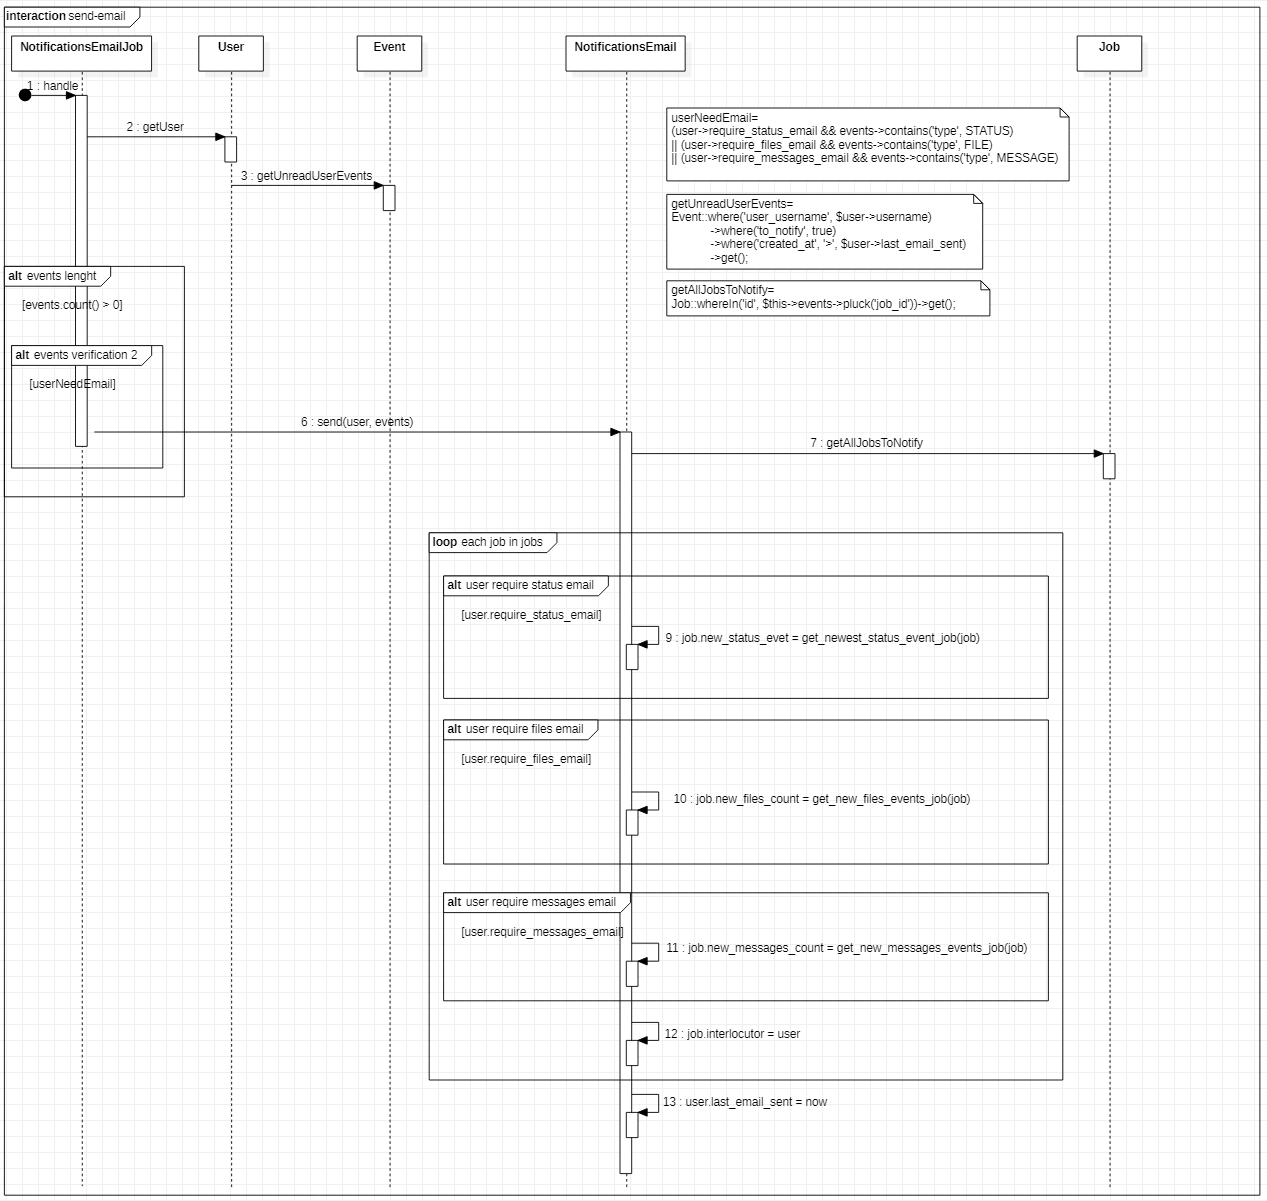
\includegraphics[width=\textwidth]{./assets/figures/emails-events-sequence.png}
        \caption{Diagramme de séquence pour la génération d'un email \label{events-email-sequence}}
    \end{figure}
\end{center}

Le but principal de ce schéma est de montrer que seuls les événements de l'application sont utilisés pour déterminer si un email doit être envoyé à l'utilisateur ou non.

En plus de tout ceci, il est également nécessaire de configurer le fichier de config "mail.php" afin que l'on puisse utiliser le service mail de la \Gls{heig-vd} en production. Cette configuration est disponible sur la figure \ref{config-mail}.

\begin{listing}[h]
    \inputminted{php}{assets/code/mail.php}
    \caption{Configuration ajoutée au fichier mail.php \label{config-mail}}
\end{listing}

Dernier point sur ce sujet, la classe "NotificationsEmail" créé un email en utilisant une vue réalisée grâce à \href{https://laravel.com/docs/9.x/blade}{Laravel Blade} et disponible sous "/resources/views/mails/email.blade".

% cliffhanger
Maintenant, que nous avons vu comment mettre en place des emails, nous allons passé au dernier point spécifique de cette application, les Websockets.

\section{Websockets}
Pour que notre application soit réactive, dans le sens où un utilisateur n'ait pas besoin de raffraichir la page afin de voir apparaître les changements qu'une autre personne aurait pu apporter sur une donnée observée, le choix des webosckets avait été réalisé. \\
Une solution classique pour contrer le problème énoncer, est d'utiliser un service externe, comme \href{https://pusher.com/}{"pusher"} recevant les changements du bakcend et les propageants au frontend via des canaux. \\
Le système utiliser est basé sur le même principe, mais au lieu d'utiliser directement "pusher", la librairie permet de lancer un serveur websockets imitant celui de pusher et donc d'éviter de passer par un service externe non maîtriser et potentiellement payant. \\
Cette librairie est nommée \href{https://beyondco.de/docs/laravel-websockets/getting-started/introduction}{"Laravel Websockets"}. Un guide de mise en place est disponible et c'est celui que j'ai suivi.

Pour mettre en place ce système de Webosckets, j'ai d'abord défini tous les événements ("Events") qui pouvait intervenir et être utiliser par les Webosckets. Je me suis inspiré de \href{https://laravel.com/docs/9.x/events}{la documentation Laravel sur les "Events"} pour les créer et réaliser.
Ces scénarii sont disponibles sur la figure \ref{ws-conception-notifications.drawio}. \\
Un Event est au final un objet contenant le canal sur lequel il doit être envoyé et les données qu'il doit envoyer.

\figi{ws-conception-notifications.drawio}{16cm}{Conception des événements pour les Websockets}

Un exemple de code d'un "Event" est disponible à la figure \ref{event-exemple}. \\
Comme expliqué précédemment, on remarque la méthode "broadcastOn" retournant le channel sur lequel doit être transmis les données lorsque cet événement intervient. \\
On peut également remarquer l'utilisation de l'interface "ShouldBroadcastNow" permettant d'émettre la diffusion de l' "Event" de façon synchrone.

\begin{listing}[h]
    \inputminted{php}{assets/code/JobAssignedEvent.php}
    \caption{Exemple d'un "Event" avec le "JobAssignedEvent" \label{event-exemple}}
\end{listing}

Il a ensuite fallu configurer ces différents channels comme utilisé sur la figure précédente \ref{event-exemple}. Ces définitions de channels sont réalisées dans le fichier "/routes/channels.php" que l'on peut consulter sur la figure \ref{ws-channels}. \\
Dans ce fichier, les channels défini possède une fonction qui détermine si l'utilisateur le droit ou non de se connecter au channel.

\begin{listing}[h]
    \inputminted{php}{assets/code/channels.php}
    \caption{Channels pour le Broadcast sur les Websockets \label{ws-channels}}
\end{listing}

Un "Event" peut ensuite être envoyer / broadcast grâce à l'instruction suivante:
\begin{verbatim}
    broadcast(new JobClosedEvent($job));
\end{verbatim}

Finalement, il est nécessaire de configurer les fichiers de config liés au \Gls{broadcast} et aux \Gls{websockets}, ces derniers se trouvent dans le dossier "/config". \\
Le premier fichier à configurer est nommé "broadcasting.php" est se voit ajouter la configuration disponible sur la figure \ref{ws-broadcasting}. \\
Il est important de remarquer que le maximum de données sont associées aux valeurs données dans le ".env" afin d'éviter de changer le code entre la phase de développement et la release pour que cela soit adapté à la production. \\
Cette manière de faire permet d'avoir un fichier ".env" pour le développement et un fichier ".env" pour la production et donc ne jamais toucher / changer le code pour faire fonctionner l'un ou l'autre.

\begin{listing}[h]
    \inputminted{php}{assets/code/broadcasting.php}
    \caption{Fichier de configuration pour le broadcasting \label{ws-broadcasting}}
\end{listing}

Le second fichier à configurer est nommé "webosckets.php" est se voit ajouter la configuration disponible sur la figure \ref{ws-broadcasting}. \\
Comme pour le premier fichier et pour les mêmes raisons, un maximum de données sont associées aux valeurs données dans le ".env". \\
On peut remarquer les lignes "verify_peer" et "verify_peer_name" qui sont à false afin d'accepter les certificats autosignés.

\begin{listing}[h]
    \inputminted{php}{assets/code/websockets.php}
    \caption{Fichier de configuration pour les Websockets \label{ws-websockets}}
\end{listing}

Un point important qui sera discuté plus tard dans le rapport, est que je n'ai malheureusement pas réussi à faire fonctionner la configuration en production. \\
Au niveau local, le  \Gls{backend} semble bien réussir à se connecter au webosckets et y propager des "Events", cependant le \Gls{frontend} ne semble pas les recevoir. \\
J'ai pu vérifier ceci grâce à la console mise à disposition par la librairie et accessible au chemin "/laravel-websockets", ainsi qu'avec des console.log du côté \Gls{frontend}.

% cliffhanger
Maintenant que nous en avons finalement terminé avec l'implémentation du \Gls{backend}, nous aimerions savoir comment tester ce dernier et être certain de son bon fonctionnement et c'est exactement ce que nous allons voir au prochain chapitre.

% ensuite décrire ce qu'on a mis en place et indiquer s'il y a des failles

% surtout indiquer tout ce qu'on a fait et tout ce que j'ai pas fait
% et pourquoi je l'ai pas fait, pas compris qqch ou pas eu le temps, pas la priorité, pas de sources suffisantes

%dans le texte (Labrecque, 2018)
%\cite{labrecque}

%suivantes:
%(Labrecque, 2018; x, yyyy;)
%pour reformuler

%Labrecque M. (2018). Pros and cons of Docker. in \textit{Docker, planet drupal}. consulté à %l'adresse: https://affinitybridge.com/blog/pros-and-cons-docker (consulté le 31.03.2022)

\chapter{Tests}
Dans ce chapitre, nous allons nous concentrer sur les tests réalisés et prévus pour l'application. \\
Le premier point important étant que seul des tests automatisés on été prévus pour le \Gls{backend}. Il a été estimé que des tests automatisés sur la partie graphique du \Gls{frontend} prendrai trop de temps et ne serait pas rentable car le frontend peut changer rapidement et demanderai beaucoup de temps pour également adapter les tests. \\
Cependant, des tests du système global ont été rédigés, comme nous le verrons plus tard.

\section{Tests automatiques}

Les tests automatiques réalisés peuvent être séparés en deux types:
\begin{itemize}
    \item les tests unitaires,
    \item les tests d'intégration;
\end{itemize}

\subsection{Tests unitaires}
Les tests unitaires ont été uniquement réalisé sur les \Gls{regex}, ces derniers permettant de valider le bon fonctionnement de la validation d'entrée utilisateurs.

On peut retrouver ces tests dans le dossier "/tests/Unit".

\subsection{Tests d'intégration}
Les tests d'intégration ont été réalisés sur toutes les routes majoritairement utilisées par les utilisateurs. Ces tests sont des tests dit "end-to-end" et ont été réalisés en suivant \href{https://laravel.com/docs/9.x/http-tests}{la documentation Laravel à ce sujet}.

Des tests sur la validation de fichiers upload ont également été réalisés.

On peut retrouver tous ces tests dans le dossier "/tests/Feature". Chaque dossier contient les tests réalisés sur une ressource / modèle. Chaque fichier représente les tests sur une action / route précise.

\subsection{Protocole de tests}
Comme mentionné précédemment, un protocole de tests a été rédigé. Ce dernier a pour but de tester globalement l'application, que cela soit en production ou en développement. \\
On peut comparer ce protocole à des tests "système". \\
Ce dernier est disponible en annexe. \\
Ce protocole est une adaptation de celui réaliser par monsieur Lieberherr.

% cliffhanger
Les tests réalisés, voyant maintenant comment réaliser une \Gls{ci} avec dans le prochain chapitre.

\chapter{Intégration continue}
L'intégration continue ou CI a fait l'objet d'un prototype afin de tester le bon fonctionnement
avant de l'intégrer au projet final.\\
Ce prototype a subit plusieurs itérations, il a fallu partir d'une CI simple permettant de juste
exécuter des tests sur un base de données SQLLite sans migration. Puis il a fallu ajouter une base
de données MySQL pour reproduire le véritable environnement. Finalement il a fallu intégrer les
migrations et les seeders afin de donner l'opportunité de tester au mieux l'application.\\
Ayant un dépôt Gitub pour le code, la CI a été réalisée avec Github Actions.\\
La CI est consultable sur les figures \ref{ci-1} et \ref{ci-2}

\begin{listing}[h]
    \inputminted{yaml}{assets/code/ci-1.yml}
    \caption{CI pour Laravel \label{ci-1}}
\end{listing}

\begin{listing}[h]
    \inputminted{yaml}{assets/code/ci-2.yml}
    \caption{CI pour Laravel \label{ci-2}}
\end{listing}

\section{Déclenchement de la CI}
La première partie après le mot clé "on", indique quand cette CI et donc cette Github Actions est
déclanchée.\\

\section{Infrastructure et services}
Ensuite, il est nécessaire d'indiquer sur quel type de machine on souhaite faire tourner notre
installation et nos tests. Il faut également construire les services nécessaires au bon
fonctionnement des tests. Ici nous construisons un SGBD MySQL, ainsi qu'une base de données.\\

\section{Étapes de configuration}

À partir du mot clé "steps", une série d'étape de configuration a lieu.\\
Chaque étape est décrite après le mot clé "name"\\
Tout d'abord, on lance les Github Actions, puis on réalise une étape non obligatoire mais
importante, on vérifie si la connexion à MySQL construit plus tôt fonctionne.\\
Il est notamment important d'installer tout l'environnement php.\\
Il faut ensuite générer les clés pour l'appluication, puis lancer les migrations et le
seeding.\\
Il est ensuite important de changer les permissions pour le storage. Et finalement il est possible
de lancer tous les tests de l'application avec phpunit.

\section{Code coverage}

\chapter{Déploiement}

\section{Déploiement continu}

\chapter{Reprise du projet}

\section{Récupération physique du projet}

\section{Erreurs restantes}

vérification des fichiers avec le mime type de php
vérification du contenu des fichiers compressés
fonctionnement des websockets en local et production
fonctionnement des emails retardés en procution

\section{Améliorations possibles}
voir toutes les issues nice to have

%%if
%\chapter{Bibliographie}
%\section{Citations et bibliographie}
%Citer vos sources est essentiel. Avec \texttt{biblatex} vous pouvez facilement citer des articles, des livres ou des sites internet. Toutes les citations dans le texte seront automatiquement regroupées en fin de document dans la section \guillemotleft Bibliographie\guillemotright. Par exemple, citons un article d'Einstein \cite{einstein} ou le livre de Dirac \cite{dirac}.

%Parfois il peut être utile d'utiliser un gestionnaire de bibliographie. La communauté académique recommande l'outil \href{https://www.zotero.org/}{Zotero} qui permet de gérer une bibliothèque numérique d'ouvrages et de références numériques. Il permet également de générer une bibliographie compatible avec \LaTeX.


%\mintinline{latex}{\SI{42.12}{\kilo\gram\metre\per\square\second}}\par
%%fi

\chapter{Conclusion}

%%if
%Bien que non nécessaire dans un rapport de Bachelor, la discussion finale d'un projet résume les résultats obtenus et dresse une conclusion objective du projet. Un manager de société est souvent amené à lire de nombreux rapport, il ne s'intéresse généralement qu'à l'introduction au contexte de l'étude et à sa conclusion.

%Il est de coutume de signer la conclusion...
%%fi

\section{Conclusion intermédiaire}
Je pense être en bonne voie pour le projet. J'ai bien saisi les concepts du framework Laravel et
vais pouvoir me plonger pleinement dans le code.\\
La première partie du projet contenant beaucoup d'analyse et de rédaction, désormais
passée, me permettra également de passer plus temps pour la réalisation du projet.\\
J'ai eu quelques soucis d'estimation du travail lors de la première réalisation du planning. J'ai pu
les corriger afin de mieux visualiser la suite du projet.\\
Mon ressenti principal sur le projet est simple, plus je me plonge dans une tâche, plus j'ai
l'impression qu'elle prendra du temps, et potentiellement plus que prévu initalement. C'est
pourquoi, j'ai essayé de prévoir plus de temps qu'en premier lieu, pour chacune de mes tâches.\\
J'ai aussi l'impression de mieux en mieux prendre en main le framework Laravel et par ce fait,
commencer à être plus productif.\\

\section{Sources d'informations}
Lors d'un projet de développement informatique, beraucoup de recherches sont réalisées lors de la
phase de développement. Il est impossible de citer toutes les sources utilisées, mais il est
important de citer les forums les plus utilisés, ainsi que les documentations.\\
Voici donc une liste de références:

\begin{itemize}
    \item laravel.com : documentation de Laravel \cite{laravel},
    \item stackoverflow.com : forum mondial numéro un pour les programmeurs \cite{stackoverflow},
    \item w3schools.com : documentation et exemples pour HTML, CSS et JavaScript \cite{w3schools},
    \item digitalocean.com : Tutoriels, pour Docker, Apache et Ubuntu \cite{digitalocean},
    \item keycloak.org: documentation de l'outil d'authentification Keycloak utilisé par la HEIG-VD,
    \item switch.ch : toute la procédure pour l’utilisation de Shibboleth et Switch edu-id \cite{switch},
    \item stackshare.io : outil pour comparer des technologies ou utils \cite{stackshare},
    \item wikipedia.org: site d'informations.
\end{itemize}

\vfil
\hspace{8cm}\makeatletter\@author\makeatother\par
\hspace{8cm}\begin{minipage}{5cm}
    %%if
    % Place pour signature numérique
    \printsignature
    %%fi
\end{minipage}
\clearpage

\appendix
\appendixpage
\addappheadtotoc

%%if
\chapter{Planning}

\begin{landscape}
    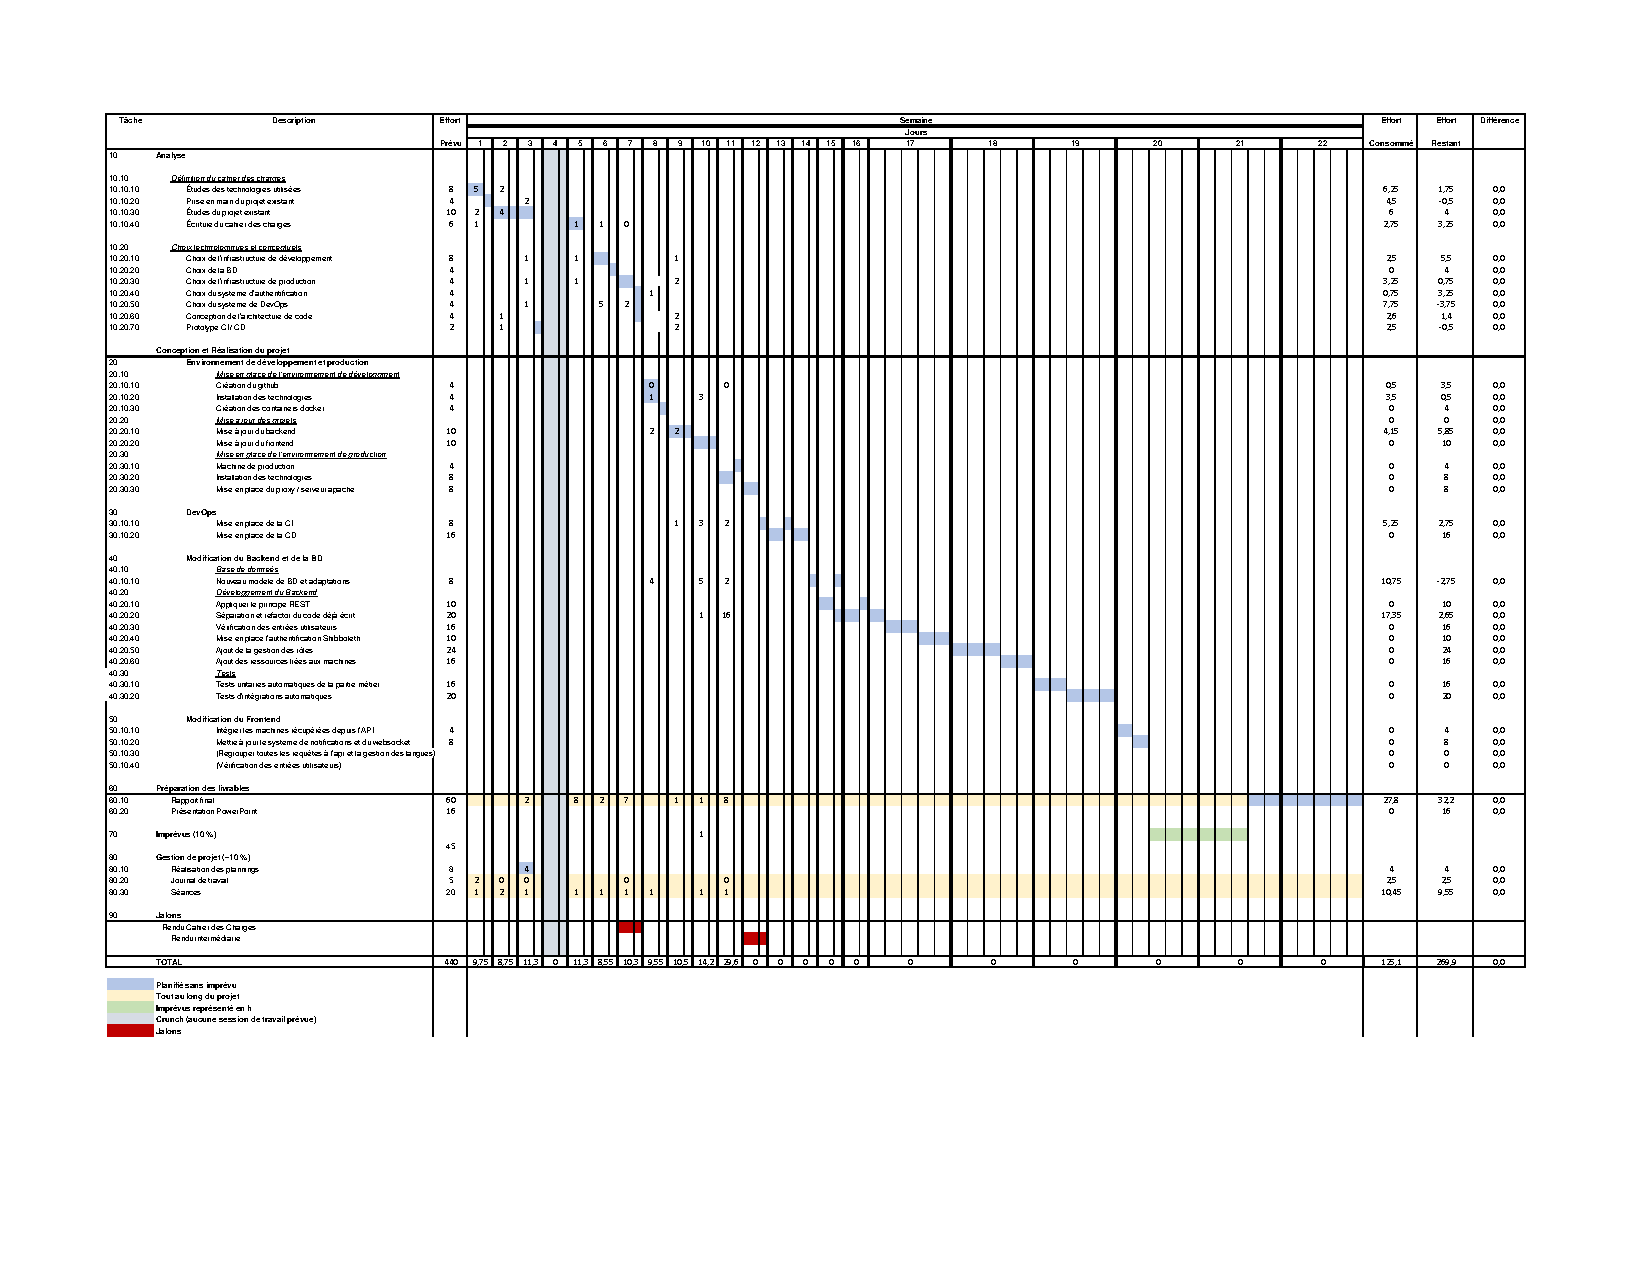
\includepdf{./assets/annexes/planning-v1.pdf}
\end{landscape}

\begin{landscape}
    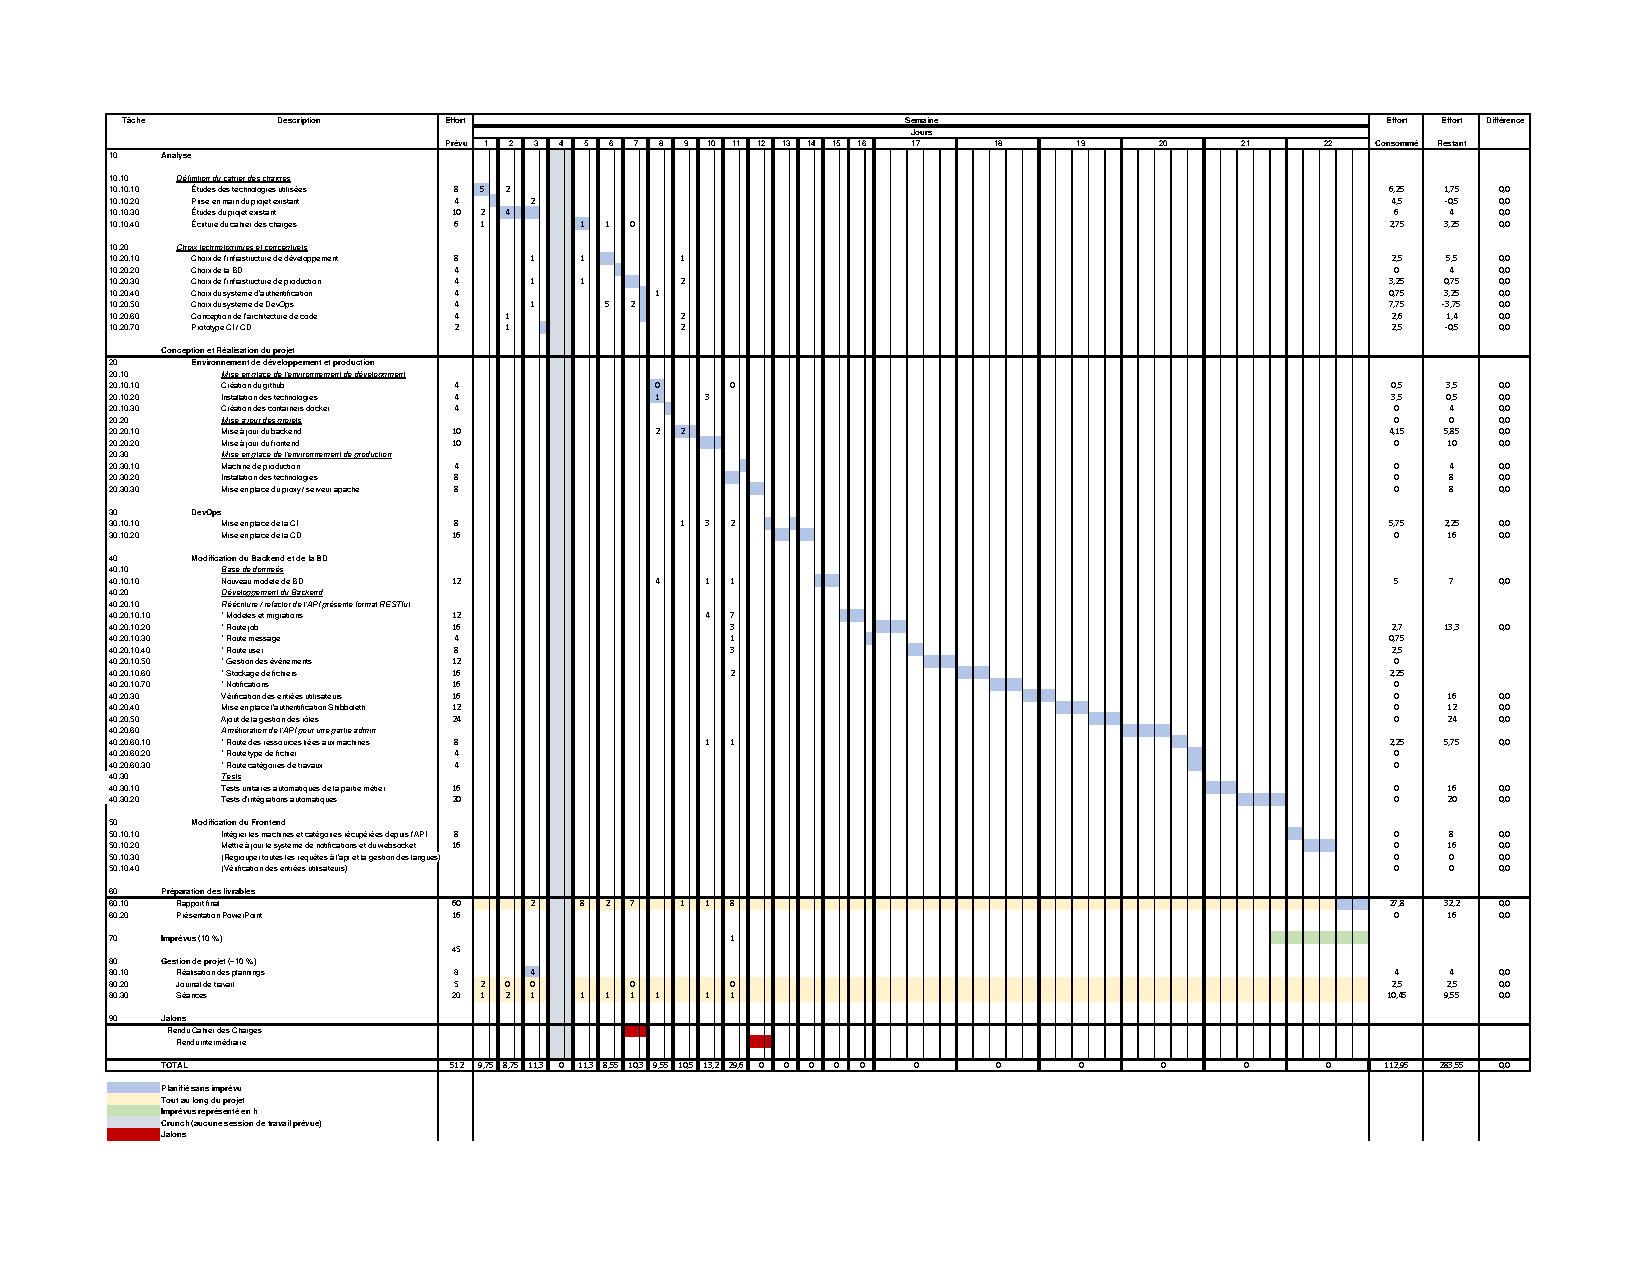
\includepdf{./assets/annexes/planning-v2.pdf}
\end{landscape}

\begin{landscape}
    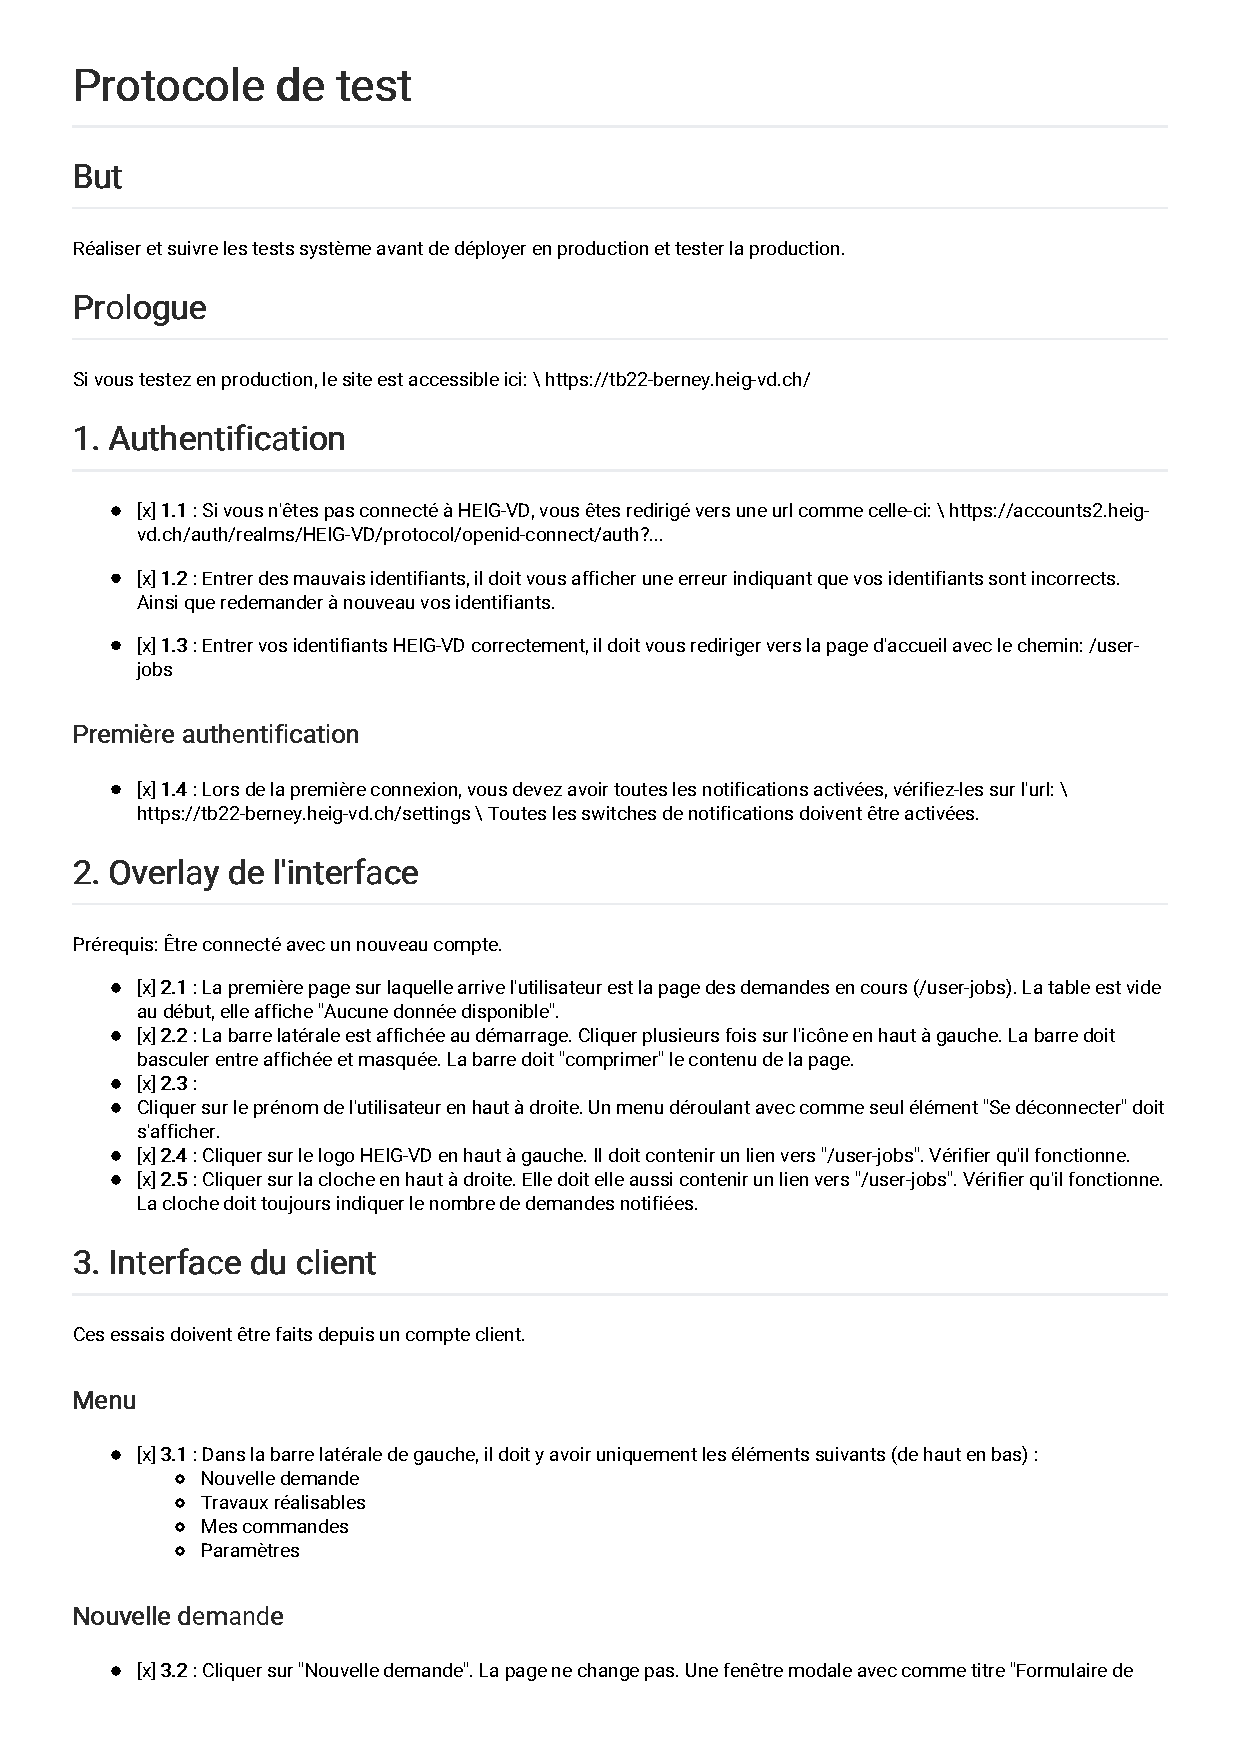
\includepdf{./assets/annexes/test-protocole.pdf}
\end{landscape}

\begin{listing}[h]
    \inputminted{php}{assets/code/13_create_roles_table.php}
    \caption{Migration de la table "roles" \label{migrations-roles}}
\end{listing}

\begin{listing}[h]
    \inputminted{php}{assets/code/14_create_users_table.php}
    \caption{Migration de la table "users" \label{migrations-users}}
\end{listing}

\begin{listing}[h]
    \inputminted{php}{assets/code/15_create_job_categories_table.php}
    \caption{Migration de la table "job-categories" \label{migrations-job-categories}}
\end{listing}

\begin{listing}[h]
    \inputminted{php}{assets/code/16_create_jobs_table.php}
    \caption{Migration de la table "jobs" \label{migrations-jobs}}
\end{listing}

\begin{listing}[h]
    \inputminted{php}{assets/code/17_create_events_table.php}
    \caption{Migration de la table "events" \label{migrations-events}}
\end{listing}

\begin{listing}[h]
    \inputminted{php}{assets/code/18_create_files_table.php}
    \caption{Migration de la table "files" \label{migrations-files}}
\end{listing}

\begin{listing}[h]
    \inputminted{php}{assets/code/19_create_messages_table.php}
    \caption{Migration de la table "messages" \label{migrations-messages}}
\end{listing}

\begin{listing}[h]
    \inputminted{php}{assets/code/20_create_device_job_category_table.php}
    \caption{Migration de la table "device-job-category" \label{migrations-device-job-category}}
\end{listing}

\begin{listing}[h]
    \inputminted{php}{assets/code/21_create_file_type_job_category_table.php}
    \caption{Migration de la table "file-type-job-category" \label{migrations-file-type-job-category}}
\end{listing}

\begin{listing}[h]
    \inputminted{php}{assets/code/22_create_role_user_table.php}
    \caption{Migration de la table "role-user" \label{migrations-role-user}}
\end{listing}

\begin{listing}[h]
    \inputminted{php}{assets/code/KeycloakGuard.php}
    \caption{KeycloakGuard \label{keycloak-guard}}
\end{listing}

%Les annexes n'ont pas un contenu \underline{normatif} mais \underline{descriptif}. Tout contenu annexé ne doit pas être nécessaire à la bonne compréhension du travail.

%Les annexes contiennent généralement :

%\begin{itemize}
%    \item les dessins mécaniques (mises en plan);
%    \item les schémas électriques détaillés;
%    \item des photographies du projet;
%    \item des scripts et des extraits de code source;
%    \item des documents techniques \pex \emph{datasheet};
%    \item des développements mathématiques.
%\end{itemize}
%\section{Sous section}
%\lipsum[1]
%%fi

\let\cleardoublepage\clearpage
\backmatter

\label{glossaire}
\printnoidxglossary
\printbibliography
\label{index}
\printindex

\end{document}
